% !TeX spellcheck = en_US
\documentclass[11pt,a4paper,twocolumn]{book}
\usepackage[latin1]{inputenc}
\usepackage{amsmath}
\usepackage{amsfonts}
\usepackage{amssymb}
\usepackage{graphicx}
\usepackage[table]{xcolor}
\usepackage{wrapfig}
\usepackage{multicol}
\usepackage{multirow}
\usepackage{paralist}
\usepackage{longtable}
\usepackage{tabu}
\usepackage{soul}
\usepackage{titling}
\usepackage{pdfpages}
\usepackage[hidelinks]{hyperref}

\hypersetup{
	colorlinks,
	citecolor=black,
	filecolor=black,
	linkcolor=black,
	urlcolor=black
}

\title{Magic Codex}
\date{\today} 

\begin{document}
	
	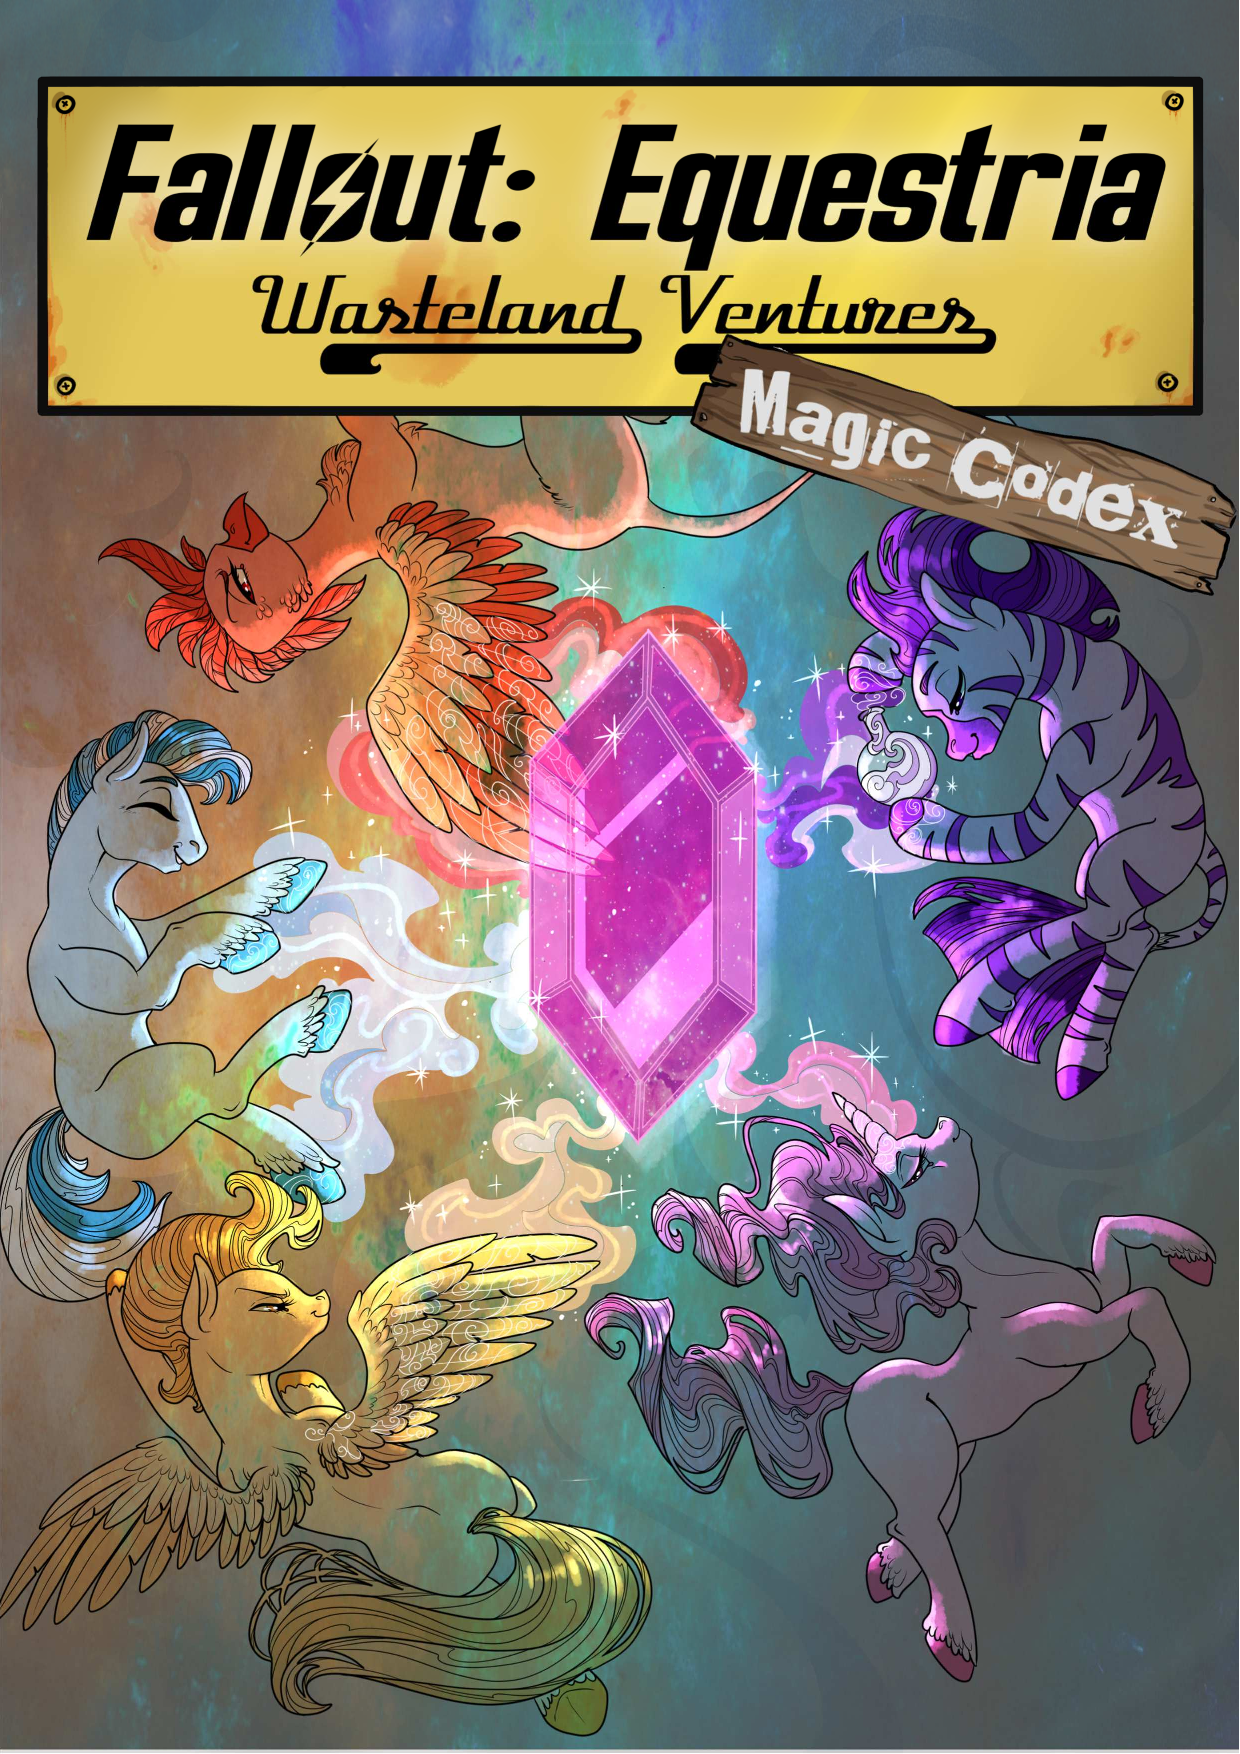
\includepdf[pages={1}]{WORD/COVER-MAGICOD.pdf}		
	\onecolumn
	\setcounter{page}{1}	
	\begin{center}
		Compiled by Waak, Kireanikin, LaPa, Miksu \& SourCherry
		
		10 AP rule basis by Yondalor
		
		Token HP \& Status rule bases by LZ
		
		\bigskip		
		\textbf{Playtesting and Advice:} LZ, Moonlight, Mittens, Kittyfluff, Ray\_Lionheart, f1r3w4rr10r, Tierney Kelly, Eden, Kendallkun, Pesian, Raven, dumbhat, GODOG, Borealis
		
		\bigskip
		\textbf{Cover and Graphics:} SourCherry
		
		\bigskip
		\textbf{Layout:} Waak \& SourCherry
		
		\bigskip
		\emph{	Special thanks to:}
		
		\emph{	Kkat - for the fanfiction that sprouted a community}
			
		\emph{	Sunrise - for the original ruleset where all started}
	\end{center}
	
	\vfill
	
	\begin{center}
		\textbf{Version 1.4.2}
		
		\emph{Last compiled on \thedate}
        
        \emph{\textbf{Contact:} wasteland-ventures@googlegroups.com}
     
	\end{center}	
    \begin{figure*}[bp]
		\centering
		
\includegraphics[width=3cm]{ART/ISA_Logo}
	\end{figure*}

	\twocolumn
	\tableofcontents

% Use chapters & Sections as follows:
% Spell category (Unicorn, Zebra) - Chapter (Should automatically switch to new page.)
% Spell School - Section
% Individual spell - subsection
%
% In shamanism, you can get creative ~Waak
% Unnumbered sections (marked with *) are not added to TOC. Use the following to force a section to be added:
% \addcontentsline{toc}{<chapter | section | subsection>}{<section title>}

\chapter{Aerial Maneuvers}    

\section*{Basic Maneuvers} 
\addcontentsline{toc}{section}{Basic Maneuvers}


\subsection*{Buccaneer Blaze [AGI]}
\addcontentsline{toc}{subsection}{Buccaneer Blaze [AGI]}

% This table set-up works, you can utilize this across the document ~Waak
{
	\rowcolors{1}{gray!30}{gray!10}
	\begin{tabu} to 75mm{| X[l,4] | X[l,7] |}
		\hline
		School 			& Agility (AGI) \\
        AP Cost	      	& All 			\\
        Strain Cost     & 4 			\\
        Range     		& - 			\\
        Target      	& AoE 			\\
        Area of Effect  & Small Burst 	\\
        Duration     	& Instant 		\\
		Position After  & On Ground     \\ \hline
	\end{tabu}
		
}

\medskip
The flier flies around a cloud in top speed, gathering electricity for one turn and upon second turn, dives towards enemy as if Sprinting. When the character comes to a halt, she releases an Area of Effect - lightning attack on a Small Burst template. Thaumaturgy is rolled on the second turn.

The second turn follows the same rules as regular Sprinting. The first turn doesn't spend AP, but the next turn's performing of the aerial sprint consumes all of the flier's AP for that turn. This Electric AoE attack deals Potency*2+10+(3) damage to non-robots, Robots take three times the damage and Power Armor takes twice the damage.

If the Thaumaturgy roll fails, the the flier ends up prone on the ground, but with electricity still gathered onto them, giving a shock to any melee or unarmed attackers that hit her for that Round. This electric attack deals AGI+5+(3) damage. After the execution Round, the electricity disperses.

% vertical fill, to avoid odd spacing, and forcing 2 spells / page (max)


\subsection*{Cloud Manipulation [CHA]}
\addcontentsline{toc}{subsection}{Cloud Manipulation [CHA]}
% Table
{
	\rowcolors{1}{gray!30}{gray!10}
	\begin{tabu} to 75mm{| X[l,4] | X[l,7] |}
		\hline
		School 			& Charisma (CHA) 	\\
        AP Cost	      	& 5 				\\
        Strain Cost     & 3 				\\
        Range     		& - 				\\
        Target      	& AoE 				\\
        Area of Effect  & Varies 			\\
        Duration     	& Instant 			\\
		Position After  & In air 			\\ \hline
	\end{tabu}
		
}

\medskip
The flyer can manipulate clouds to different effects, such as causing momentary weather effects or striking all enemies with lightning-bolts. Thaumaturgy roll is used to determine success. Area of effect is determined by the flier's Potency as shown below: 

% Use List environment in these:
% \begin{itemize} OR \begin{compactitem} OR \begin{description}
% Use "\item" before each entry, on its own line ~Waak
%
% Example Below:
% \begin{description}
% 	\item[$<$10 Potency] Tiny Burst area
% \end{description}
\begin{quote}
  \begin{description}
    \item[$<$10 Potency] 	Tiny Burst area
    \item[11-20 Potency] 	Small Burst area
    \item[21+ Potency] 	Large Burst area
  \end{description}
\end{quote}

\noindent
Lightning bolts and hail deal 30+(3) damage.

\vfill


\subsection*{Contrail [AGI]}
\addcontentsline{toc}{subsection}{Contrail [AGI]}
%Table
{
	\rowcolors{1}{gray!30}{gray!10}
	\begin{tabu} to 75mm{| X[l,4] | X[l,7] |}
		\hline
		School 			& Agility (AGI) 	\\
        AP Cost	      	& Movement 			\\
        Strain Cost     & 2 				\\
        Range     		& - 				\\
        Target      	& Self 				\\
        Area of Effect  & - 	 			\\
        Duration     	& 2 Rounds 	 		\\
		Position After  & In air 			\\ \hline
	\end{tabu}
		
}

\medskip

Flier flies fast enough to create a contrail behind them, and flies low enough to distract their enemy, giving all enemies they fly past a Distraction, its severity determined by the flier's Potency. Flier must fly in a straight line. The enemies will suffer from a visibility penalty of -10 for 2 turns.

\begin{quote}
  \begin{description}
    \item[$<$10 Potency] 	Tiny Burst area
    \item[11-20 Potency] 	Small Burst area
    \item[21+ Potency] 	Large Burst area
  \end{description}
\end{quote}


\subsection*{Creeping Barrage [AGI]}
\addcontentsline{toc}{subsection}{Creeping Barrage [AGI]}
% Table
{
	\rowcolors{1}{gray!30}{gray!10}
	\begin{tabu} to 75mm{| X[l,4] | X[l,7] |}
		\hline
		School 			& Agility (AGI) 	\\
        AP Cost	      	& 5 + Weapon 		\\
        Strain Cost     & 3 				\\
        Range     		& - 				\\
        Target      	& AoE 				\\
        Area of Effect  & Line, [Potency]*2 meters 	 	\\
        Duration     	& Instant 	 		\\
		Position After  & In air 			\\ \hline
	\end{tabu}
		
}

\medskip

The flier speeds up, flying towards the enemy and bombarding them with gunfire or magical energy, targeting enemies in a line at the maximum of Potency*2 meters (Potency hexes).

The Maneuver requires a successful Firearms/MEW roll in addition to Thaumaturgy roll. The weapon must be Full-Auto weapon.
If the Thaumaturgy roll fails, the flier ends up on the ground, knocked prone, but doesn't lose AP from trying to perform the maneuver. However, they will lose Strain. If the Firearms/MEW roll fails, the flier has performed the maneuver, but misses the targets.


\subsection*{Defensive Spiral [END]}
\addcontentsline{toc}{subsection}{Defensive Spiral [END]}
% Table
{
	\rowcolors{1}{gray!30}{gray!10}
	\begin{tabu} to 75mm{| X[l,4] | X[l,7] |}
		\hline
		School 			& Endurance (END) 	\\
        AP Cost	      	& All 				\\
        Strain Cost     & 5 				\\
        Range     		& - 				\\
        Target      	& AoE 				\\
        Area of Effect  & Varies 	 		\\
        Duration     	& 1 round	 		\\
		Position After  & In air 			\\ \hline
	\end{tabu}
		
}

\medskip

The flier flies low to the ground, in a circle with a maximum size determined by her Potency, protecting all allies inside the circle with the air pressure from their flight. Allies inside the circle have extra 10 DT until caster's next turn. The affected area is determined by flier's Potency.

To perform this maneuver, the flier must successfully roll Thaumaturgy -20 or be flown off course for 10 meters (5 hexes) and get knocked prone in a random direction.

GM decides the direction a failed maneuverer flies towards with a roll of the dice, 1d6 for each main direction. If they crash against someone, they take damage according to the falling template.

\begin{quote}
  \begin{description}
    \item[$<$10 Potency] 	Tiny Burst area
    \item[11-20 Potency] 	Small Burst area
    \item[21+ Potency] 	Large Burst area
  \end{description}
\end{quote}

The flier can maintain this Spiral for a single turn, and must rest their wings for the next turn - they cannot perform maneuvers but can still otherwise act.

\vfill


\subsection*{Defog Twirl [CHA]}
\addcontentsline{toc}{subsection}{Defog Twirl [CHA]}
% Table
{
	\rowcolors{1}{gray!30}{gray!10}
	\begin{tabu} to 75mm{| X[l,4] | X[l,7] |}
		\hline
		School 			& Charisma (CHA) 	\\
        AP Cost	      	& 4			 		\\
        Strain Cost     & 2 				\\
        Range     		& - 				\\
        Target      	& AoE 				\\
        Area of Effect  & Varies 		 	\\
        Duration     	& Instant 	 		\\
		Position After  & In air 			\\ \hline
	\end{tabu}
		
}

\medskip

Flier makes a dainty twirl near the ground, dispelling fog, poisonous clouds or put out small fires in an area determined by her Potency. Additionally, the flier may instead spread these effects to an equally sized area, in case of fire or smoke. This maneuver also removes Burning-status from all targets within the affected area. Thaumaturgy roll is required.

\begin{quote}
  \begin{description}
    \item[$<$10 Potency] 	Tiny Burst area
    \item[11-20 Potency] 	Small Burst area
    \item[21+ Potency] 	Large Burst area
  \end{description}
\end{quote}


\subsection*{Dirt Drag [END]}
\addcontentsline{toc}{subsection}{Dirt Drag [END]}
% Table
{
	\rowcolors{1}{gray!30}{gray!10}
	\begin{tabu} to 75mm{| X[l,4] | X[l,7] |}
		\hline
		School 			& Endurance (END) 	\\
        AP Cost	      	& All 				\\
        Strain Cost     & 4 				\\
        Range     		& - 				\\
        Target      	& 1 				\\
        Area of Effect  & - 	 			\\
        Duration     	& Instant 	 		\\
		Position After  & In air 			\\ \hline
	\end{tabu}
		
}

\medskip

The Flier grabs onto a target and drags the target along the ground, injuring them. This attack follows the rules of Sprinting.

Requires a successful opposed roll of flier's Thaumaturgy against the target's STR. If the target is successful, the flier ends up on the ground, in a grapple with the target. Deals Potency*2+10+(2) damage to the target if flier is successful.


\subsection*{Divebomb [END]}
\addcontentsline{toc}{subsection}{Divebomb [END]}
% Table
{
	\rowcolors{1}{gray!30}{gray!10}
	\begin{tabu} to 75mm{| X[l,4] | X[l,7] |}
		\hline
		School 			& Endurance (END) 	\\
        AP Cost	      	& All 				\\
        Strain Cost     & 4 				\\
        Range     		& - 				\\
        Target      	& 1 				\\
        Area of Effect  & - 	 			\\
        Duration     	& Instant 	 		\\
		Position After  & Adjacent to target 	\\ \hline
	\end{tabu}
		
}

\medskip

The Flier takes off up to the air and dives down, making a single powerful Melee or Unarmed attack with high chance of Knocking down the target.

Deals normal attack damage with extra Potency*2+(3) damage. Flier gets free Trip attempt after a successful hit, with bonus of +20.

%\vfill


\subsection*{Fantastic Flash [CHA]}
\addcontentsline{toc}{subsection}{Fantastic Flash [CHA]}
% Table
{
	\rowcolors{1}{gray!30}{gray!10}
	\begin{tabu} to 75mm{| X[l,4] | X[l,7] |}
		\hline
		School 			& Charisma (CHA) 	\\
        AP Cost	      	& 5 				\\
        Strain Cost     & 3 				\\
        Range     		& - 				\\
        Target      	& 1 				\\
        Area of Effect  & - 	 			\\
        Duration     	& 2 Rounds	 		\\
		Position After  & In air 			\\ \hline
	\end{tabu}
		
}

\medskip

The flier makes a straight dashing line towards the target, and takes a sharp turn upwards leaving behind a flash of bright light on a Tiny Burst area.

Thaumaturgy roll is required to successfully perform, after which an opposed roll follows; target(s) will make Opposed PER roll against flier's CHA or be Blinded for 2 turns.

If the Thaumaturgy roll fails, the character remains in air, but the effects of the maneuver do not happen. AP is depleted, but Strain is not.

\vfill


\subsection*{Fire Trail [CHA]}
\addcontentsline{toc}{subsection}{Fire Trail [CHA]}
% Table
{
	\rowcolors{1}{gray!30}{gray!10}
	\begin{tabu} to 75mm{| X[l,4] | X[l,7] |}
		\hline
		School 			& Charisma (CHA) 	\\
        AP Cost	      	& Movement	 		\\
        Strain Cost     & 3 				\\
        Range     		& - 				\\
        Target      	& AoE 				\\
        Area of Effect  & Line, CHA*2 m 	\\
        Duration     	& Potency/2 turns 	\\
		Position After  & In air 			\\ \hline
	\end{tabu}
		
}

\medskip

The flier charges towards an enemy, staying close to the ground and leaving behind a trail of fire that burns all that come into contact with it. Anyone caught in it may gain Burning status. The trail of fire lasts for Potency/2 turns. This attack is a Charge, meaning they get bonuses and penalties accordingly.

A successful Thaumaturgy roll is required to perform this Maneuver.


\subsection*{Hightail Sweep [AGI]}
\addcontentsline{toc}{subsection}{Hightail Sweep [AGI]}
% Table
{
	\rowcolors{1}{gray!30}{gray!10}
	\begin{tabu} to 75mm{| X[l,4] | X[l,7] |}
		\hline
		School 			& Agility (AGI) 	\\
        AP Cost	      	& 5 				\\
        Strain Cost     & 3 				\\
        Range     		& - 				\\
        Target      	& AoE 				\\
        Area of Effect  & Small Burst 	 	\\
        Duration     	& 2 Rounds 	 			\\
		Position After  & On the ground 	\\ \hline
	\end{tabu}
		
}

\medskip

The flier stays low to the ground towards the enemy, whipping up a dust cloud with their wings to cause a distraction in an area determined by her potency:
\begin{quote}
  \begin{description}
    \item[$<$10 Potency] 	Minor Distr.
    \item[11-20 Potency] 	Moderate distr.
    \item[21+ Potency] 		Major Distr.
  \end{description}
\end{quote}

\vfill


\subsection*{Plummet [END]}
\addcontentsline{toc}{subsection}{Plummet [END]}
% Table
{
	\rowcolors{1}{gray!30}{gray!10}
	\begin{tabu} to 75mm{| X[l,4] | X[l,7] |}
		\hline
		School 			& Endurance (END) 	\\
        AP Cost	      	& 8					\\
        Strain Cost     & 4 				\\
        Range     		& - 				\\
        Target      	& 1 				\\
        Area of Effect  & - 	 			\\
        Duration     	& Instant 	 		\\
		Position After  & In air 			\\ \hline
	\end{tabu}
		
}

\medskip

The flier grabs their target and carries them high to the sky, then throws the target plummeting towards ground. Requires a successful opposed roll of the Flier's Thaumaturgy -10 to the target's STR.

The target takes Potency*3+(4) damage, and ends up Prone on the ground. Targets beyond one (1) Size Increment larger than the flier are impossible to lift.

If the Thaumaturgy roll fails, the flier ends up on the ground in a Grapple with the target as an attacker. Both take damage according to Falling damage table due to collision.

%\vfill
\vfill

\subsection*{Sonic Rain-Nuke [END]}
\addcontentsline{toc}{subsection}{Sonic Rain-Nuke [END]}
% Table
{
	\rowcolors{1}{gray!30}{gray!10}
	\begin{tabu} to 75mm{| X[l,4] | X[l,7] |}
		\hline
		School 			& Endurance (END) 	\\
        AP Cost	      	& 8 				\\
        Strain Cost     & 4 				\\
        Range     		& - 				\\
        Target      	& AoE 				\\
        Area of Effect  & Large Burst 	 	\\
        Duration     	& Instant 	 		\\
		Position After  & On the ground 	\\ \hline
	\end{tabu}
		
}

\medskip

Flier soars high in the air, then dives down to deliver a shock wave that explodes in a multi-colored mushroom cloud when a successful Thaumaturgy roll is made.
Initial blast deals Potency*3+(5) damage. Everyone caught in the attack may attempt to stay upright from the blast with a successful STR -1 roll, or be knocked prone from the attack.

If the flier is a ghoul, they inflict an additional 1 Rad at 3x40\% alongside the damage, however, this will deplete their accumulated rads by half to a minimum of 1.


\subsection*{Sun Celebration [CHA]}
\addcontentsline{toc}{subsection}{Sun Celebration [CHA]}
% Table
{
	\rowcolors{1}{gray!30}{gray!10}
	\begin{tabu} to 75mm{| X[l,4] | X[l,7] |}
		\hline
		School 			& Charisma (CHA) 	\\
        AP Cost	      	& 5/6 				\\
        Strain Cost     & 4 				\\
        Range     		& - 				\\
        Target      	& All enemies 		\\
        Area of Effect  & - 	 			\\
        Duration     	& 2 Turns 	 		\\
		Position After  & In air 			\\ \hline
	\end{tabu}
		
}

\medskip

Sun Celebration is a bit more difficult of a maneuver to pull off in the often-cloudy Wasteland: As her first action, the flier must disperse clouds from a Small Burst area with a Thaumaturgy check. Dispersing the clouds costs 5 AP, and the dispersed clouds gather after 5 turns.

As her second action, she positions herself in front of the sun to deal a Distraction to all who look upon her, and fail a PER roll. The positioning costs 6 AP, and this Distraction lasts for 2 Turns. 

\begin{quote}
  \begin{description}
    \item[$<$10 Potency] 	Minor Distr.
    \item[11-20 Potency] 	Moderate Distr.
    \item[21+ Potency] 	Major Distr.
  \end{description}
\end{quote}


\subsection*{Tactical Weather Manipulation [CHA]}
\addcontentsline{toc}{subsection}{Tactical Weather Manipulation [CHA]}
% Table
{
	\rowcolors{1}{gray!30}{gray!10}
	\begin{tabu} to 75mm{| X[l,4] | X[l,7] |}
		\hline
		School 			& Charisma (CHA) 	\\
        AP Cost	      	& 3 				\\
        Strain Cost     & 2 				\\
        Range     		& - 				\\
        Target      	& AoE 				\\
        Area of Effect  & Varies 	 		\\
        Duration     	& Potency Rounds	\\
		Position After  & In air 			\\ \hline
	\end{tabu}
		
}

\medskip

Flier can further worsen or improve the weather conditions, making visibility in a in an area one step further from current visibility condition. For example, a light drizzle of rain (-5 Visibility penalty) would become a downpour (-10 Visibility Penalty) if worsened, or clear skies (no penalty) if improved. The maximum area that is affected by this spell is determined by the caster's potency. Thaumaturgy roll is required. 

\begin{quote}
  \begin{description}
    \item[$<$10 Potency] 	Tiny Burst area
    \item[11-20 Potency] 	Small Burst area
    \item[21+ Potency] 	Large Burst area
  \end{description}
\end{quote}

\vfill

\subsection*{Tornado [AGI]}
\addcontentsline{toc}{subsection}{Tornado [AGI]}
% Table
{
	\rowcolors{1}{gray!30}{gray!10}
	\begin{tabu} to 75mm{| X[l,4] | X[l,7] |}
		\hline
		School 			& Agility (AGI) 	\\
        AP Cost	      	& Attack	 		\\
        Strain Cost     & 4 				\\
        Range     		& Potency*2 m 		\\
        Target      	& 1 				\\
        Area of Effect  & - 	 			\\
        Duration     	& Instant 	 		\\
		Position After  & Start 			\\ \hline
	\end{tabu}
		
}

\medskip

The flier makes a circular flight around the target, striking them with Melee or Unarmed attacks. Flier returns to the same location where she set off at the beginning of the maneuver.

Costs the combined AP cost of all attacks. However, Flier has -5 AP less to use during her next turn. Flier may use Special Attacks granted by her weapons.

This Maneuver does not provoke attacks of opportunity. Failed Thaumaturgy roll will end the maneuver after first strike on an adjacent hex around the target, and will not cause her to have -5 AP less on her next turn.

\subsection*{Twister [END]}
\addcontentsline{toc}{subsection}{Twister [END]}
% Table
{
	\rowcolors{1}{gray!30}{gray!10}
	\begin{tabu} to 75mm{| X[l,4] | X[l,7] |}
		\hline
		School 			& Endurance (END) 	\\
        AP Cost	      	& All 				\\
        Strain Cost     & 4 				\\
        Range     		& - 				\\
        Target      	& 1 				\\
        Area of Effect  & - 	 			\\
        Duration     	& Instant 	 		\\
		Position After  & Target's original position 		\\ \hline
	\end{tabu}
		
}

\medskip

The Flier grabs the target and spins them around, throwing them END*2 meters (END hexes) away, damaging them and anything they hit along the way. Target may not be larger than one size category to the flier. Smaller targets fly further, END + Size category of hexes.

Requires a successful opposed roll of flier's Thaumaturgy against the target's STR.

Deals Potency*2+(3) damage to the target and anything they hit.


\subsection*{Weave Defense [AGI]}
\addcontentsline{toc}{subsection}{Weave Defense [AGI]}
% Table
{
	\rowcolors{1}{gray!30}{gray!10}
	\begin{tabu} to 75mm{| X[l,4] | X[l,7] |}
		\hline
		School 			& Agility (AGI) 	\\
        AP Cost	      	& 3 				\\
        Strain Cost     & 1 				\\
        Range     		& - 				\\
        Target      	& Self 				\\
        Area of Effect  & - 	 			\\
        Duration     	& 2 Rounds	 			\\
		Position After  & In air 			\\ \hline
	\end{tabu}
		
}

\medskip

Flier weaves in the air as they fly, giving all enemies that target her a Distraction penalty when targeting her, rolled with a Thaumaturgy roll.

\begin{quote}
  \begin{description}
    \item[$<$10 Potency] 	Minor Distr.
    \item[11-20 Potency] 	Moderate Distr.
    \item[21+ Potency] 	Major Distr.
  \end{description}
\end{quote}

\vfill

\section*{Wonderbolt \& Talon Maneuvers}
\addcontentsline{toc}{section}{Wonderbolt \& Talon Maneuvers}

\subsection*{Blackwing's Mettle}
\addcontentsline{toc}{subsection}{Blackwing's Mettle}
% Table
{
	\rowcolors{1}{gray!30}{gray!10}
	\begin{tabu} to 75mm{| X[l,4] | X[l,7] |}
		\hline
		School 			& Talon (AGI/END/CHA) 			\\
        AP Cost	      	& 6 				\\
        Strain Cost     & 6 				\\
        Range     		& - 				\\
        Target      	& Allies 			\\
        Area of Effect  & - 	 			\\
        Duration     	& Potency/3 turns 	 \\
		Position After  & In air 			\\ \hline
	\end{tabu}
		
}

\medskip

The flier takes to the sky, scouting the area for hostile targets' precise positions and relaying the info back to their team with a intricate flight pattern. A Thaumaturgy -10 roll is required to execute this maneuver.

The intricate flight pattern is automatically known by other player characters, but ally NPC's have to decipher the meaning with a successful PER-1 roll.
This Aerial Maneuver gives +5 to combat skills and +5 DT to the allies, but doesn't benefit the flier. If the Thaumaturgy roll fails, the flier becomes a target for the opponents, with the enemy getting a +10 in combat skills to attack the flier.


\subsection*{Carrion's Blight}
\addcontentsline{toc}{subsection}{Carrion's Blight}
% Table
{
	\rowcolors{1}{gray!30}{gray!10}
	\begin{tabu} to 75mm{| X[l,4] | X[l,7] |}
		\hline
		School 			& Talon (AGI/END/CHA)			\\
        AP Cost	      	& 9 				\\
        Strain Cost     & 6 				\\
        Range     		& - 				\\
        Target      	& AoE 				\\
        Area of Effect  & Small Burst 	 	\\
        Duration     	& 3 Rounds	 	\\
		Position After  & In air 			\\ \hline
	\end{tabu}
		
}

\medskip

The flier performs a shift in air pressure causing a considerable dizziness to targets in a Small Burst template.
Target must make an opposed END-2 roll against fliers END. Afflicted targets have all their actions cost 2 AP more and suffer from Medium Distraction, for 3 turns.

If Flier is a ghoul, Radiation is also emitted, with 2 Rads at 2x60\%. This also depletes their radiation reserves completely.


\subsection*{Commander Easyglider's Esprit de Corps}
\addcontentsline{toc}{subsection}{Commander Easyglider's Esprit de Corps}
% Table
{
	\rowcolors{1}{gray!30}{gray!10}
	\begin{tabu} to 75mm{| X[l,4] | X[l,7] |}
		\hline
		School 			& Wonderbolt (AGI/END/CHA) 		\\
        AP Cost	      	& All 				\\
        Strain Cost     & 6 				\\
        Range     		& - 				\\
        Target      	& AoE 				\\
        Area of Effect  & Large Burst 	 	\\
        Duration     	& 3 Rounds	 			\\
		Position After  & In air 			\\ \hline
	\end{tabu}
		
}

\medskip

The Flier makes a series of stunning and complicated flying routines, either inspiring their allies or intimidating their opponents in a Large Burst template for 3 turns. Thaumaturgy -20 roll is required for successful maneuvering.

Before executing the maneuver, the flier must decide if they want to boost their allies or demoralize their enemies. On a success, the effects he has chosen happen.

\begin{itemize}
  \item	If the Flier boosts their allies, they gain +10 to all Skill and SPECIAL rolls.
  \item If the Flier demoralizes their enemies, the enemies get a -10 to all skills and SPECIAL rolls.
  \item If the Thaumaturgy roll unsuccessful, all, including the Flier, in the Large Burst Area get a Minor Distraction.
\end{itemize}

\vfill


\subsection*{Fleetfoot's Fix-it-up}
\addcontentsline{toc}{subsection}{Fleetfoot's Fix-it-up}
% Table
{
	\rowcolors{1}{gray!30}{gray!10}
	\begin{tabu} to 75mm{| X[l,4] | X[l,7] |}
		\hline
		School 			& Wonderbolt (AGI/END/CHA)		\\
        AP Cost	      	& 6 				\\
        Strain Cost     & 6 				\\
        Range     		& - 				\\
        Target      	& Self 				\\
        Area of Effect  & -	 				\\
        Duration     	& Potency/2 rounds	 	\\
		Position After  & In air 			\\ \hline
	\end{tabu}
		
}

\medskip

The flier steels her nerves and makes a daringly quick spiral, ignoring any crippled limb she has to carry the fight to the end. Requires a successful Thaumaturgy -30 check to execute.

On a success, the flier ignores one Crippled limb penalty of her choosing for an Potency/2 number of rounds. On a failure, the flier loses 2 HP from stressing her bruised body.


\subsection*{Gawd's Glorious Featherbedding}
\addcontentsline{toc}{subsection}{Gawd's Glorious Featherbedding}
% Table
{
	\rowcolors{1}{gray!30}{gray!10}
	\begin{tabu} to 75mm{| X[l,4] | X[l,7] |}
		\hline
		School 			& Talon (AGI/END/CHA)			\\
        AP Cost	      	& All 				\\
        Strain Cost     & 6 				\\
        Range     		& - 				\\
        Target      	& AoE 				\\
        Area of Effect  & Huge Burst 	 	\\
        Duration     	& Potency/4 Rounds 	\\
		Position After  & In air 			\\ \hline
	\end{tabu}
		
}

\medskip

The Flier makes a grand display of agile and charming, enticing movements, giving allies a morale bonus to SPECIAL and Skill rolls.

On a success, the flier grants a bonus of +10 to all SPECIAL and Skill rolls for Potency/4 amount of turns to everyone in Huge Burst Template. A failed roll instead causes a Minor Distraction to all creatures within Huge Burst Template.



\subsection*{General Firefly's Double Inside-Out Loop}
\addcontentsline{toc}{subsection}{General Firefly's Double Inside-Out Loop}
% Table
{
	\rowcolors{1}{gray!30}{gray!10}
	\begin{tabu} to 75mm{| X[l,4] | X[l,7] |}
		\hline
		School 			& Wonderbolt (AGI/END/CHA) 		\\
        AP Cost	      	& 5 + Weapon 		\\
        Strain Cost     & 6 				\\
        Range     		& - 				\\
        Target      	& 1 				\\
        Area of Effect  & - 	 			\\
        Duration     	& Instant 	 		\\
		Position After  & In air 			\\ \hline
	\end{tabu}
		
}

\medskip

The flier attacks their target once during the low-flight part of the first loop, picks up speed to perform the second loop where they descend onto the same target to trample them.

The maneuver requires a Thaumaturgy -20 roll to succeed. On a success, the flier may attack one opponent twice with a Melee or Unarmed weapon, both attacks costing -1 AP (minimum of 1 AP). The opponent may gain Stunned status after the second attack, if successful. On a failure, she may only attack once with normal AP cost, and ends her maneuver adjacent to her target.

%\vfill

\vfill

\subsection*{Gilda's Feline Frenzium Furiatus}
\addcontentsline{toc}{subsection}{Gilda's Feline Frenzium Furiatus}
% Table
{
	\rowcolors{1}{gray!30}{gray!10}
	\begin{tabu} to 75mm{| X[l,4] | X[l,7] |}
		\hline
		School 			& Talon (AGI/END/CHA)			\\
        AP Cost	      	& Unarmed Attack 	\\
        Strain Cost     & 6 				\\
        Range     		& Varies 		\\
        Target      	& 1 				\\
        Area of Effect  & - 	 			\\
        Duration     	& Instant 	 		\\
		Position After  & In air 			\\ \hline
	\end{tabu}
		
}

\medskip

The Flier dashes towards a target, flying around then and striking them like a murder of crows or pride of lions, with the use of her beak and talons.

The flier can attack multiple targets within an area determined by her Potency. She strikes with Unarmed attacks as many times as her AP pool allows, with all attacks costing 1 AP less (minimum 1) and dealing additional +(1) damage. She may choose to attack one target or multiple, and after she is unable to attack she ends up adjacent to the last target of her maneuver. The remaining AP cannot be spent on any actions.

At the end of her turn, the flier can choose to continue the maneuver on her next turn. She must make an AGI/END/CHA roll to successfully keep the maneuver going, with a cumulative penalty of 1 after each successive round. If the roll is unsuccessful, she will fall to the ground and is knocked prone.

\begin{quote}
	\begin{description}
		\item[$<$10 Potency] 	10 m / 5 hex
		\item[11-20 Potency] 	20 m / 10 hex
		\item[21+ Potency] 	30 m / 15 hex
	\end{description}
\end{quote}

\vfill

\subsection*{Henrietta's Threatful Bravura}
\addcontentsline{toc}{subsection}{Henrietta's Threatful Bravura}
% Table
{
	\rowcolors{1}{gray!30}{gray!10}
	\begin{tabu} to 75mm{| X[l,4] | X[l,7] |}
		\hline
		School 			& Talon (AGI/END/CHA)			\\
        AP Cost	      	& All				\\
        Strain Cost     & 6 				\\
        Range     		& - 				\\
        Target      	& AoE 				\\
        Area of Effect  & Large Burst 	 	\\
        Duration     	& 1/2 Rounds	 			\\
		Position After  & On the ground 	\\ \hline
	\end{tabu}
		
}

\medskip

The Flier takes a hovering position in the air, sending gusts of powerful winds in a Large Burst template, causing Medium Distraction. Those within the area of the maneuver can make an opposed END roll against flier's AGI/END/CHA to only suffer a Minor Distraction. Anyone going in or through the area of effect must also do the opposed roll. If Flier has the perk \textit{Roar}, she can combine effects of both to cause the distraction last an additional turn, and on a critical roll, cause a Major Distraction instead. 

The maneuver costs all of the flier's AP. Maneuver ends at her next turn, leaving her on the ground with 5 AP less, and inability to use her wings till the next turn.

\subsection*{Rainbow Dash's Sonic Rainboom}
\addcontentsline{toc}{subsection}{Rainbow Dash's Sonic Rainboom}
{
	\rowcolors{1}{gray!30}{gray!10}
	\begin{tabu} to 75mm{| X[l,4] | X[l,7] |}
		\hline
		School 			& Wonderbolt (AGI/END/CHA)		\\
        AP Cost	      	& All 				\\
        Strain Cost     & 6 				\\
        Range     		& - 				\\
        Target      	& AoE 				\\
        Area of Effect  & Huge Burst 	 	\\
        Duration     	& Instant 	 		\\
		Position After  & In air 			\\ \hline
	\end{tabu}
		
}

\medskip

The flier picks up speed from her current position, flying straight up fast enough to break the sound barrier and release a multi-colored sonic boom. This sonic boom causes clouds to disperse and deals damage to all in a Huge Burst template. Requires a successful Thaumaturgy -20 check to execute.

The attack deals Potency*4+(5) damage. If the flier is a ghoul, they instead perform the Sonic Radboom, which, in addition to damage and cloud dispersing deals 2 Rads at 5x60\%. This will deplete the flier's Radiation Tracker completely.

\subsection*{Spitfire's Icarian Sun Salutation}
\addcontentsline{toc}{subsection}{Spitfire's Icarian Sun Salutation}
% Table
{
	\rowcolors{1}{gray!30}{gray!10}
	\begin{tabu} to 75mm{| X[l,4] | X[l,7] |}
		\hline
		School 			& Wonderbolt (AGI/END/CHA)		\\
        AP Cost	      	& All 		\\
        Strain Cost     & 6 				\\
        Range     		& - 				\\
        Target      	& AoE 				\\
        Area of Effect  & Small Burst 	 	\\
        Duration     	& Instant 	 		\\
		Position After  & On the ground 	\\ \hline
	\end{tabu}
		
}

\medskip

This attack requires either the sun or a large source of heat, such as an advancing forest fire. The flier flies close enough to the fiery object to be set on fire, after which the flier will speed up and ram their opponent and spreading the fire at any adjacent characters in a Small Burst Area. Thaumaturgy -10 roll is required for successful maneuvering.

When successfully performing this maneuver, the initial opponent takes Potency*2+(5) damage and may be inflicted with Burning status, with -1 END to resist. Any characters sans performer may also get Burning status but do not otherwise take damage. After the Maneuver, the performer is on the ground. If the performer fails their Thaumaturgy roll, they get the Burning-status instead and take damage accordingly.

\vfill

\subsection*{Surprise's Sneak Sweep}
\addcontentsline{toc}{subsection}{Surprise's Sneak Sweep}
% Table
{
	\rowcolors{1}{gray!30}{gray!10}
	\begin{tabu} to 75mm{| X[l,4] | X[l,7] |}
		\hline
		School 			& Wonderbolt (AGI/END/CHA)		\\
        AP Cost	      	& All 				\\
        Strain Cost     & 6 				\\
        Range     		& Huge Burst		\\
        Target      	& 1 				\\
        Area of Effect  & - 	 			\\
        Duration     	& Instant 	 		\\
		Position After  & Ground 			\\ \hline
	\end{tabu}
		
}

\medskip

The flier carries a single target, an ally or an enemy, to a more favorable position in the battlefield. The flier chooses one target within Huge Burst Template, making a Thaumaturgy -20 check.

On a success, the flier flies to the target, picks it up and moves it up to her Potency*2 meters (Potency hexes) from the target's original position, ending up adjacent to the target after the maneuver. On a failure, the flier ends up knocked prone next to her target, having not moved it at all. Targets beyond one (1) Size Increment larger than the flier are impossible to lift.

\chapter{Earth Pony Magic}


\section*{Adrenaline Rush [STR]}
\addcontentsline{toc}{section}{Adrenaline Rush [STR]}
% Table
{
	\rowcolors{1}{gray!30}{gray!10}
	\begin{tabu} to 75mm{| X[l,4] | X[l,7] |}
		\hline
		School 			& Strength (STR) 	\\
        AP Cost	      	& 5 				\\
        Strain Cost     & 2 				\\
        Range     		& - 				\\
        Target      	& Self 				\\
        Area of Effect  & - 	 			\\
        Duration     	& Potency/3 turns 	\\ \hline
	\end{tabu}
		
}

\medskip

The earth pony gets themselves into a frenzy of hormones to swap a Pain Threshold status effect for Enraged- status effect for a short while. A successful Thaumaturgy roll is required for casting this spell.

After the duration of the spell ends, the Pain Threshold status returns along with an additional -1 penalty on STR and END for Potency/3 turns.

This spell can only be done once per combat.

\vfill

\section*{Cheer [CHA]}
\addcontentsline{toc}{section}{Cheer [CHA]}
% Table
{
	\rowcolors{1}{gray!30}{gray!10}
	\begin{tabu} to 75mm{| X[l,4] | X[l,7] |}
		\hline
		School 			& Charisma (CHA) 	\\
        AP Cost	      	& 4 				\\
        Strain Cost     & 3 				\\
        Range     		& Potency*2 m 		\\
        Target      	& Allies 			\\
        Area of Effect  & CHA/2 number of allies	 			\\
        Duration     	& 3 turns 			\\ \hline
	\end{tabu}
		
}

\medskip

Caster inspires [CHA]/2 number of allies with a magically enchanted praise. A successful Thaumaturgy roll is required for casting this spell.

The caster chooses which one of the following boons she will give, if successful:

\medskip
\begin{compactitem}
  \item +10 to a single non-combat skill, except Thaumaturgy
  \item +5 to a single combat skill
  \item +5 to Thaumaturgy-skill
  \item +1 to CHA
  \item +10 to Carry Weight
  \item Move 2 meters (1 hex) for free
\end{compactitem}

\medskip
A new Cheer-bonus given to a character will replace the old one.

\vfill


\section*{Comforting Words [CHA]}
\addcontentsline{toc}{section}{Comforting Words [CHA]}
% Table
{
	\rowcolors{1}{gray!30}{gray!10}
	\begin{tabu} to 75mm{| X[l,4] | X[l,7] |}
		\hline
		School 			& Charisma (CHA) 	\\
        AP Cost	      	& 3 				\\
        Strain Cost     & 5 				\\
        Range     		& Potency/2 m 		\\
        Target      	& 1 Target 			\\
        Area of Effect  & - 	 			\\
        Duration     	& Instant		 	\\ \hline
	\end{tabu}
		
}

\medskip

The sensible Earth Pony uses their innate magic fueled into their voice to help a single ally to calm down from a Panic-Pain Threshold during combat situations. The character doesn't suffer from a Pain Threshold until they take further damage.

Outside of combat, this spell can be used to lower one's Insanity by 1 point, to a minimum of 0. If the target has acquired half or more of their maximum Insanity points, the caster suffers a -10 to their Thaumaturgy roll.

When used to overcome Insanity, this spell cannot be used again in 24 hours to lower Insanity, but can be used to calm down a target from Panic. A critically successful Thaumaturgy-roll causes the Insanity to lower by 2.

If the Insanity-lowering effect is used on an opponent, a CHA Opposed roll is required. If successful, the opponent temporarily becomes more lucid, but not necessarily docile.

\begin{verse}
	\textbf{Example:} Shining Example attempts to use Comforting Words to lower Maabara's Insanity, after she suffered a devastating blow to her psyche courtesy of in-game events. Maabara's maximum insanity is 6, and she currently has 4 points. Because Maabara has more than half of her maximum Insanity points, Shining Example's Thaumaturgy suffers a penalty of -10 to successfully perform this spell.
\end{verse}


\section*{Crash this Barn [STR]}
\addcontentsline{toc}{section}{Crash this Barn [STR]}
% Table
{
	\rowcolors{1}{gray!30}{gray!10}
	\begin{tabu} to 75mm{| X[l,4] | X[l,7] |}
		\hline
		School 			& Strength (STR) 	\\
        AP Cost	      	& 5 				\\
        Strain Cost     & 4 				\\
        Range     		& Adjacent 			\\
        Target      	& AoE 				\\
        Area of Effect  & See text 	 		\\
        Duration     	& Instant 			\\ \hline
	\end{tabu}
		
}

\medskip

The earth pony enchants the muscles on their hind legs and kicks a cover to remove it entirely from an area determined by Potency:

\begin{quote}
  \begin{description}
    \item[$<$10 Potency] 	4 meters/2 hex
    \item[11-20 Potency] 	6 meters/3 hex
    \item[21+ Potency] 	8 meters/4 hex
  \end{description}
\end{quote}

Only covers with 20 DT or under can be destroyed. A successful Thaumaturgy roll is required for casting this spell.

\textbf{Note:} This can also be utilized out of combat to knock holes into obstacles or kicking in doors. Same limits apply.

\vfill


\section*{Earthly Warning [PER]}
\addcontentsline{toc}{section}{Earthly Warning [PER]}
% Table
{
	\rowcolors{1}{gray!30}{gray!10}
	\begin{tabu} to 75mm{| X[l,4] | X[l,7] |}
		\hline
		School 			& Perception (PER)	\\
        AP Cost	      	& 6 				\\
        Strain Cost     & 5 				\\
        Range     		& - 				\\
        Target      	& Self 				\\
        Area of Effect  & - 	 			\\
        Duration     	& Potency minutes 	\\ \hline
	\end{tabu}
		
}

\medskip

The Earth Pony receives small magical cues from the earth itself, giving her cryptic warnings of possible danger such as tail twitching or shaky hoof. A successful Thaumaturgy roll is required for casting this spell.

In combat, this spell gives an extra penalty of 5 to first dodge action.

Outside of combat, this spell gives a +1 to AGI to dodge falling objects or creatures about to crash you, as well as +1 to PER to detect ambushes and traps.

\textbf{Example:} Shining Example uses Earthly Warning to dodge an enemy's action, using 2 AP to dodge, normally giving the enemy -10 to attack. With Earthly Warning, Shining Example gets an additional 5 added to this penalty, making the enemy's attack penalty -15 instead.


\section*{Enchanted Hooves [STR]}
\addcontentsline{toc}{section}{Enchanted Hooves [STR]}
% Table
{
	\rowcolors{1}{gray!30}{gray!10}
	\begin{tabu} to 75mm{| X[l,4] | X[l,7] |}
		\hline
		School 			& Strength (STR) 	\\
        AP Cost	      	& 5 				\\
        Strain Cost     & 2 				\\
        Range     		& - 				\\
        Target      	& Self 				\\
        Area of Effect  & - 	 			\\
        Duration     	& Potency minutes 	\\ \hline
	\end{tabu}
		
}

\medskip

Ignore the +1 AP cost of Difficult Terrain and Movement AP costs on Climbing and Crawling are reduced by 1. A successful Thaumaturgy roll is required for casting this spell.

In addition, the character can now charge in Difficult Terrain.


\section*{Enhance Plant [CHA]}
\addcontentsline{toc}{section}{Enhance Plant [CHA]}
% Table
{
	\rowcolors{1}{gray!30}{gray!10}
	\begin{tabu} to 75mm{| X[l,4] | X[l,7] |}
		\hline
		School 			& Charisma (CHA) 	\\
        AP Cost	      	& 5 				\\
        Strain Cost     & 4 				\\
        Range     		& - 				\\
        Target      	& Up to CHA number of plants 				\\
        Area of Effect  & - 	 			\\
        Duration     	& - 	\\ \hline
	\end{tabu}
		
}

\medskip

The caster can enhance the qualities of up to [CHA] number of plants, such as giving a thorny plant longer thorns and making the plant more damaging, a poisonous plant enhanced with a more potent toxin or a fresh fruit tree to become more nutritious.
A successful Thaumaturgy roll is required for casting this spell.

The spell requires that the plant in question has been planted in soil, either in the ground or in a flower pot for the spell to work.

The mechanical effects of this spell should be discussed with the GM as it is case-by-case basis on what plants are in the area. It is to be noted that this spell cannot be used to make plants Rad-free.

Most of these magical effects are difficult to spot, but a successful -10 Thaumaturgy or -2 INT roll will reveal the enhanced nature of the plant.
Once the spell is cast, the effect will remain on the plant indefinitely unless a Failsafe-spell is cast or the original caster decides to cancel the effect.

Character can only have up to [CHA] number of enchanted plants, and if she wishes to enhance a new plant, a previously enhanced plant loses its enhancement, chosen by the caster. Canceling the spell doesn't cost AP.

\vfill

\section*{Find Poison [PER]}
\addcontentsline{toc}{section}{Find Poison [PER]}
% Table
{
	\rowcolors{1}{gray!30}{gray!10}
	\begin{tabu} to 75mm{| X[l,4] | X[l,7] |}
		\hline
		School 			& Perception (PER) 	\\
        AP Cost	      	& 6 				\\
        Strain Cost     & 4 				\\
        Range     		& Large Burst Area 	\\
        Target      	& Self 				\\
        Area of Effect  & - 	 			\\
        Duration     	& Potency*2 m 		\\ \hline
	\end{tabu}
		
}

\medskip

The caster gains a +10 bonus on their Survival for identifying poisons around them, be it poisonous creatures, tainted food or poisonous gases, and can pinpoint their location. In addition, they gain 5\% to their poison resistance.

A successful Thaumaturgy roll is required for casting this spell.


\section*{Fortify (STR)}
\addcontentsline{toc}{section}{Fortify [STR]}
% Table
{
	\rowcolors{1}{gray!30}{gray!10}
	\begin{tabu} to 75mm{| X[l,4] | X[l,7] |}
		\hline
		School 			& Strength (STR) 	\\
        AP Cost	      	& 5 				\\
        Strain Cost     & 4 				\\
        Range     		& - 				\\
        Target      	& Self 				\\
        Area of Effect  & - 	 			\\
        Duration     	& Potency/2 turns 	\\ \hline
	\end{tabu}
		
}

\medskip

Earth Pony's body is enchanted to gain one of the following bonuses to aid them for a period of time:
\begin{itemize}
  \item +5 DT to resist a single elemental damage source such as fire or ice
  \item +1 END to resist Status Effects
  \item +10 to Poison Resistance
  \item +10 to Rad Resistance
  \item +1 to STR/+10 to Unarmed to Grapple
\end{itemize}
	
A successful Thaumaturgy roll is required for casting this spell. A new Fortify-bonus replaces the old one.

\vfill

\section*{Healing Hooves [CHA]}
\addcontentsline{toc}{section}{Healing Hooves [CHA]}
% Table
{
	\rowcolors{1}{gray!30}{gray!10}
	\begin{tabu} to 75mm{| X[l,4] | X[l,7] |}
		\hline
		School 			& Charisma (CHA) 	\\
        AP Cost	      	& 10 				\\
        Strain Cost     & 6 				\\
        Range     		& - 				\\
        Target      	& 1 Ally 			\\
        Area of Effect  & - 	 			\\
        Duration     	& Potency/2 turns 	\\ \hline
	\end{tabu}
		
}

\medskip

Earth pony draws the energies from the earth and directs it towards their ally, giving one of the following:
The following effects do not resume after the spell ends:

\begin{itemize}
  \item Heal a physical status effect, such as Bleeding.
  \item Help an Unconscious ally back on their feet.
  \item Ally has SPECIAL damage healed by caster's [CHA]/2 amount.
\end{itemize}

The following effects resume after the spell ends:

\begin{itemize}
  \item Ally can ignore one Crippled-condition for the duration of the spell.
  \item Ally can ignore one Pain Threshold penalty for the duration of the spell.
\end{itemize}
	
A successful Thaumaturgy roll is required for casting this spell.

\vfill


\section*{Improve Obstacle [PER]}
\addcontentsline{toc}{section}{Improve Obstacle [PER]}
% Table
{
	\rowcolors{1}{gray!30}{gray!10}
	\begin{tabu} to 75mm{| X[l,4] | X[l,7] |}
		\hline
		School 			& Perception (PER) 	\\
        AP Cost	      	& 7 				\\
        Strain Cost     & 6 				\\
        Range     		& Adjacent 			\\
        Target      	& Cover/Obstacle 	\\
        Area of Effect  & - 	 			\\
        Duration     	& Potency/2 turns 	\\ \hline
	\end{tabu}
		
}

\medskip

The Earth Pony channels their inner magic to enchant a Cover to be stronger than it was for [Potency]/2 number of turns. A successful Thaumaturgy roll is required for casting this spell. A critical success on Thaumaturgy- skill roll upgrades the Cover by additional +5 DT.

The amount of DT that the Earth Pony can improve the cover with is dependent on their current Potency as follows:

\begin{quote}
  \begin{description}
    \item[$<$10 Potency] 	5 DT
    \item[11-20 Potency] 	10 DT
    \item[21+ Potency] 	20 DT
  \end{description}
\end{quote}


\section*{Inner Circle [CHA]}
\addcontentsline{toc}{section}{Inner Circle [CHA]}
% Table
{
	\rowcolors{1}{gray!30}{gray!10}
	\begin{tabu} to 75mm{| X[l,4] | X[l,7] |}
		\hline
		School 			& Charisma (CHA) 	\\
        AP Cost	      	& +2 AP to attached spell 				\\
        Strain Cost     & +2 Strain to attached spell 			\\
        Range     		& - 				\\
        Target      	& - 				\\
        Area of Effect  & Small Burst area 	\\
        Duration     	& 3 turns 			\\ \hline
	\end{tabu}
		
}

\medskip

Allows the Earth pony to share the effects of the next self-targeting spell she casts with [CHA]/2 number of allies. However, these allies must be close to the caster for this spell's effect to work, as the spell is centered on the caster. When using this spell in tandem with a spell, it adds +2 to the spells' original AP cost and Strain cost.

A successful Thaumaturgy roll is required for casting this spell.


\section*{Mend [STR]}
\addcontentsline{toc}{section}{Mend [STR]}
% Table
{
	\rowcolors{1}{gray!30}{gray!10}
	\begin{tabu} to 75mm{| X[l,4] | X[l,7] |}
		\hline
		School 			& Strength (STR) 	\\
        AP Cost	      	& 10 				\\
        Strain Cost     & 6 				\\
        Range     		& - 				\\
        Target      	& Self 				\\
        Area of Effect  & - 	 			\\
        Duration     	& 24 hours 			\\ \hline
	\end{tabu}
		
}

\medskip

The caster mends themselves by pulling the nutrients from the soil beneath them and converting it into a healing energy with their magic, accelerating their healing process. A successful Thaumaturgy roll is required for casting this spell.

After the spell's effect has ended, the caster cannot recast this spell in the next 24 hours from that.

The number of extra HP tokens healed with Natural Healing is determined by the caster's Potency as follows:
\begin{quote}
  \begin{description}
    \item[$<$10 Potency] 	1 HP
    \item[11-20 Potency] 	2 HP
    \item[21+ Potency] 	3 HP
  \end{description}
\end{quote}

When used in tandem with Inner Circle -spell, allies' healed HPs are determined by their own Potency (STR) values, not that of the caster.

\vfill


\section*{Overgrow [STR]}
\addcontentsline{toc}{section}{Overgrow [STR]}
% Table
{
	\rowcolors{1}{gray!30}{gray!10}
	\begin{tabu} to 75mm{| X[l,4] | X[l,7] |}
		\hline
		School 			& Strength (STR) 	\\
        AP Cost	      	& 6 				\\
        Strain Cost     & 6 				\\
        Range     		& Potency*2 m 		\\
        Target      	& -					\\
        Area of Effect  & Large Burst area 	\\
        Duration     	& (STR) turns 	\\ \hline
	\end{tabu}
		
}

\medskip

The caster channels their magic to the plants near them, enriching the plantlife to grow faster. A successful Thaumaturgy roll is required for casting this spell.

This spell causes a spot within the spell's range chosen by the caster to grow thick with underbrush and roots, making a Large Burst template area into a Difficult Terrain.
In addition, any creature between Size -2 and +2 has a 25\% chance of getting tripped by the plants when traversing through. Sizes 3-4 trample over the plants while sizes -3 to -4 simply slip through. When the spell ends, the plants return to their normal size.


\section*{Plant Calling [CHA]}
\addcontentsline{toc}{section}{Plant Calling [CHA]}
% Table
{
	\rowcolors{1}{gray!30}{gray!10}
	\begin{tabu} to 75mm{| X[l,4] | X[l,7] |}
		\hline
		School 			& Charisma (CHA) 	\\
        AP Cost	      	& 8 				\\
        Strain Cost     & 4 				\\
        Range     		& - 				\\
        Target      	& (CHA)/2 plants 	\\
        Area of Effect  & - 	 			\\
        Duration     	& Potency/2 turns 	\\ \hline
	\end{tabu}
		
}

\medskip

The earth pony channels their magic to compel any nearby Plant mutant to help them for the duration of the spell. If the Thaumaturgy roll fails, no Plants appear.

The plants act on the enemy's turn, and act independently from the caller, though the earth pony can give suggestions to the plant, that the mutated bush may follow through with.

After the spell ends, the plant may either flee or turn hostile.

A successful Thaumaturgy roll is required for casting this spell.


\section*{Protection of the Earth [STR]}
\addcontentsline{toc}{section}{Protection of the Earth [STR]}
% Table
{
	\rowcolors{1}{gray!30}{gray!10}
	\begin{tabu} to 75mm{| X[l,4] | X[l,7] |}
		\hline
		School 			& Strength (STR) 	\\
        AP Cost	      	& 6 				\\
        Strain Cost     & 3 				\\
        Range     		& - 				\\
        Target      	& Self 				\\
        Area of Effect  & - 	 			\\
        Duration     	& Potency minutes 	\\ \hline
	\end{tabu}
		
}

\medskip

Become immune to poison or Stunned-status effect for [Potency] number of minutes. Critical Success adds an extra 2 minutes. A successful Thaumaturgy roll is required for casting this spell.


\section*{Rooted [STR]}
\addcontentsline{toc}{section}{Rooted [STR]}
% Table
{
	\rowcolors{1}{gray!30}{gray!10}
	\begin{tabu} to 75mm{| X[l,4] | X[l,7] |}
		\hline
		School 			& Strength (STR) 	\\
        AP Cost	      	& 7 				\\
        Strain Cost     & 3 				\\
        Range     		& - 				\\
        Target      	& Self 				\\
        Area of Effect  & - 	 			\\
        Duration     	& Potency/2 turns 	\\ \hline
	\end{tabu}
		
}

\medskip

The earth pony sinks their hooves into the earth for [Potency]/2 turns, making them immune to trip attempts against them, but cannot use movement or any actions that require limbs unless they cancel this spell's effect. Enemies Size 3 and bigger have a 25\% chance of their Trip attempts to be ignored instead.

A successful Thaumaturgy roll is required for casting this spell.

\vfill


\section*{Scrutinizing Gaze [PER]}
\addcontentsline{toc}{section}{Scrutinizing Gaze [PER]}
% Table
{
	\rowcolors{1}{gray!30}{gray!10}
	\begin{tabu} to 75mm{| X[l,4] | X[l,7] |}
		\hline
		School 			& Perception (PER) 	\\
		AP Cost	      	& 5 				\\
		Strain Cost     & 3 				\\
		Range     		& - 	\\
		Target      	& Self				\\
		Area of Effect  & - 	 		\\
		Duration     	& 4 turns / 4 hours 				\\ \hline
	\end{tabu}
	
}

\medskip

The earth pony focuses on her surroundings or one specific target, finding minute details and opportunities much easier.

The caster chooses the effect they want to bestow upon themselves. This spell has use in and outside of combat.

A successful Thaumaturgy roll is required for casting this spell.

\medskip

\textbf{In combat}, the duration of this spell is shorter, with following effects available to choose from:

\medskip

\begin{compactitem}
	\item Ignore visibility penalties according to the caster's Potency
	\begin{quote}
		\begin{description}
			\item[$<$10 Potency] 	5
			\item[11-20 Potency] 	10
			\item[21+ Potency] 	15
		\end{description}
	\end{quote}
	\item Gain +1 to END to resist Blinded-status effect for the duration of this spell
	\item Ignore DT according to the caster's Potency.
	\begin{quote}
		\begin{description}
			\item[$<$10 Potency] 	5
			\item[11-20 Potency] 	10
			\item[21+ Potency] 	15
		\end{description}
	\end{quote}
	\item Caster can add their Potency to their chance of crippling a target.
\end{compactitem}

\vfill

\textbf{Outside of combat} the duration of the spell is longer, with following effects available to choose from.

\medskip

\begin{compactitem}
	\item +2 Initiative for the duration of this spell
	\item Gain +1 PER to see through disguises and lies.
	\item Ignore visibility penalties according to the caster's Potency
	\begin{quote}
		\begin{description}
			\item[$<$10 Potency] 	5
			\item[11-20 Potency] 	10
			\item[21+ Potency] 	15
		\end{description}
	\end{quote}
	\item Gain a bonus on Lockpick, Sleight and Survival according to the caster's Potency.	
	\begin{quote}
		\begin{description}
			\item[$<$10 Potency] 	5
			\item[11-20 Potency] 	10
			\item[21+ Potency] 	15
		\end{description}
	\end{quote}
\end{compactitem}

A new effect given with this spell replaces the old one.

\section*{Smart Cookie's Invocation [PER]}
\addcontentsline{toc}{section}{Smart Cookie's Invocation [PER]}
% Table
{
	\rowcolors{1}{gray!30}{gray!10}
	\begin{tabu} to 75mm{| X[l,4] | X[l,7] |}
		\hline
		School 			& Perception (PER) 	\\
        AP Cost	      	& 7 				\\
        Strain Cost     & 2 				\\
        Range     		& - 				\\
        Target      	& Self 				\\
        Area of Effect  & - 	 			\\
        Duration     	& Varies 			\\ \hline
	\end{tabu}
		
}

\medskip

The Earth Pony's Skill requirements for upgrading Schematics are halved for a number of days depending on their PER. In addition the penalty to the used skill is -20 instead of -30.

\begin{quote}
  \begin{description}
    \item[$<$10 Potency] 	1 day
    \item[11-20 Potency] 	2 days
    \item[21+ Potency] 	3 days
  \end{description}	
\end{quote}

A successful Thaumaturgy roll is required for casting this spell.

\vfill

\section*{Sound Mind [CHA]}
\addcontentsline{toc}{section}{Sound Mind [CHA]}
% Table
{
	\rowcolors{1}{gray!30}{gray!10}
	\begin{tabu} to 75mm{| X[l,4] | X[l,7] |}
		\hline
		School 			& Charisma (CHA) 	\\
        AP Cost	      	& 8 				\\
        Strain Cost     & 2 				\\
        Range     		& - 				\\
        Target      	& Self 				\\
        Area of Effect  & - 	 			\\
        Duration     	& Potency*2 minutes \\ \hline
	\end{tabu}
		
}

\medskip

The caster's chance of gaining an Insanity point is halved from 20\% to 10\% for the duration of this spell. However, this spell can only be used once per day. A successful Thaumaturgy roll is required for casting this spell. A Critically successful Thaumaturgy roll gives extra 2 minutes.


\section*{Stone Shield [STR]}
\addcontentsline{toc}{section}{Stone Shield [STR]}
% Table
{
	\rowcolors{1}{gray!30}{gray!10}
	\begin{tabu} to 75mm{| X[l,4] | X[l,7] |}
		\hline
		School 			& Strength (STR) 	\\
        AP Cost	      	& 8 				\\
        Strain Cost     & 6 				\\
        Range     		& Potency meters 	\\
        Target      	& - 				\\
        Area of Effect  & 4 meters 	 		\\
        Duration     	& - 				\\ \hline
	\end{tabu}
		
}

\medskip

The caster kicks the ground to release a small tremor in the earth, to raise up a platform to create a cover made from stone.

This spell can be used to create pathways where there are none or to otherwise manipulate terrain outside of combat.
It can also be created to make small shelters, though the result is far from comfortable lodging. Said shelter is just barely big enough to house the player party, and sleeping in it doesn't incur Sleep Deprivation. A critical success when creating the shelter gives the characters the Well-Rested status if they rest in it, due to the shelter being more secure and better crafted.

A successful Thaumaturgy roll is required for casting this spell.

\section*{Threatening Gaze [PER]}
\addcontentsline{toc}{section}{Threatening Gaze [PER]}
% Table
{
	\rowcolors{1}{gray!30}{gray!10}
	\begin{tabu} to 75mm{| X[l,4] | X[l,7] |}
		\hline
		School 			& Perception (PER) 	\\
		AP Cost	      	& 7 				\\
		Strain Cost     & 3 				\\
		Range     		& See text 	\\
		Target      	& 1 Target				\\
		Area of Effect  & - 	 		\\
		Duration     	& 2 turns 				\\ \hline
	\end{tabu}
	
}

\medskip

The earth pony puts on his fiercest gaze, as if trying to kill the target of their piercing glare alone.

The caster gives a single target in range a piercing, intimidating stare which will have one of three effects of the caster's choosing:

\begin{itemize}
	\item The target is petrified with fear for the duration of this spell, unable to move. They are still able to attack an adjacent target, but cannot make Attacks of Opportunity.
	\item The target becomes so afraid of the caster they cannot attack her for the duration of this spell.
	\item Have a $(10 + $Potency$)\%$ chance to make the target flee. Some NPCs might be immune to this effect, however.
\end{itemize}

The spell cannot be used on the same target twice.

A successful Thaumaturgy roll is required for casting this spell.

The range of this spell, centered on caster, is determined by the caster's potency as follows:
\begin{quote}
	\begin{description}
		\item[$<$10 Potency] 	Small Burst Area
		\item[11-20 Potency] 	Large Burst Area
		\item[21+ Potency] 	Huge Burst Area
	\end{description}	
\end{quote}   

\chapter{Unicorn Magic}


\section*{\#1 Assistant [CHA/INT]}
\addcontentsline{toc}{section}{\#1 Assistant [CHA/INT]}
% Table
{
	\rowcolors{1}{gray!30}{gray!10}
	\begin{tabu} to 75mm{| X[l,4] | X[l,7] |}
		\hline
		School 			& Metamagic (CHA/INT) 	\\
        AP Cost	      	& - 				\\
        Strain Cost     & 1 				\\
        Range     		& - 				\\
        Target      	& Self 				\\
        Area of Effect  & - 	 			\\
        Duration     	& Permanent 		\\ \hline
	\end{tabu}
		
}

\medskip

A magical-enhanced critter assists the caster in mundane tasks.

At one point of caster's history, she has bonded with a critter with a magical connection. The critter is a loyal companion that will never leave the caster's side, although in combat it usually hides in the caster's inventory or otherwise vanishes from the spot. It can be summoned with this spell from everywhere, and will appear through a portal to where the caster is. The critter can help their master with a myriad of tasks, including but not limited to eavesdropping, fitting into tight spaces and courier tasks.

The critter will obey its master to the best of its abilities. The critter and its master can communicate with each other, even if they wouldn't share a common language. If the master and the critter don't share interests, and if the master treats her assistant badly, there is a chance that the critter might leave its master.

If this spell is acquired at some point during a campaign, it is up to the GM where, when and how a critter assistant emerges. The type of critter that is eligible to become an assistant depends on the campaign, but generally they are small and not exotic, such as birds, rodents, dogs, cats or lizards. The size category of the critter is either -1 or -2, depending on its species.


\section*{Alarm [END]}
\addcontentsline{toc}{section}{Alarm [END]}
% Table
{
	\rowcolors{1}{gray!30}{gray!10}
	\begin{tabu} to 75mm{| X[l,4] | X[l,7] |}
		\hline
		School 			& Protective (END) 	\\
        AP Cost	      	& 5 				\\
        Strain Cost     & 2 				\\
        Range     		& Potency*2 		\\
        Target      	& AoE 				\\
        Area of Effect  & Small Burst Area 	\\
        Duration     	& Potency hours 	\\ \hline
	\end{tabu}
		
}

\medskip

Designates an area that triggers when a threatening force enters it.

The spell marks a specific area which alerts the caster to the presence of a threatening entity when it enters or passes through the area. If the caster is awake, he immediately recognizes that the spell has triggered. If she is sleeping, she must succeed in a PER check, negating any penalties from the sleep.

The spell's area can be made visible with \textbf{Detection-spell}.

\vfill


\section*{Amplify [CHA]}
\addcontentsline{toc}{section}{Amplify [CHA]}
% Table
{
	\rowcolors{1}{gray!30}{gray!10}
	\begin{tabu} to 75mm{| X[l,4] | X[l,7] |}
		\hline
		School 			& Enchantment (CHA) \\
        AP Cost	      	& 5 				\\
        Strain Cost     & 2 				\\
        Range     		& Potency*2 		\\
        Target      	& Up to 4 targets 	\\
        Area of Effect  & - 	 			\\
        Duration     	& Potency Rounds 	\\ \hline
	\end{tabu}
		
}

\medskip

Exaggerates sensory stimuli, such as sight, sound, smell or taste.

The spell increases the source of a sensory stimulus of targets. At the casting of the spell, the caster must choose one sense (sight, sound, taste, smell or touch). The targets then produce an increased effect of that sense. The spell affects up to 4 targets and they may make an END opposed roll to resist the spell.

The spell can also have a secondary effect. For example, if the caster chooses to boost her own sound, she might gain a bonus to her Intimidation check equal to her Potency.


\section*{Anesthetic [INT]}
\addcontentsline{toc}{section}{Anesthetic [INT]}
% Table
{
	\rowcolors{1}{gray!30}{gray!10}
	\begin{tabu} to 75mm{| X[l,4] | X[l,7] |}
		\hline
		School 			& Medical (INT) 	\\
        AP Cost	      	& 5 				\\
        Strain Cost     & 3 				\\
        Range     		& Touch 			\\
        Target      	& 1 Target 			\\
        Area of Effect  & - 	 			\\
        Duration     	& Potency hours/rounds 	\\ \hline
	\end{tabu}
		
}

\medskip

Caster conjures a ball of anesthetic magical energy. When the energy ball hits a target, it falls immediately into a deep slumber.

The caster must make a Medicine check. If successful, the magical energy will touch the patient correctly, and she loses her sense of touch and pain. This also results in a loss of associated motor capabilities, effectively paralyzing the patient. Duration is Potency hours on a willing or unconscious subject. During the spell's effect, the patient can be healed more efficiently, as she won't panic or tremble. Medicine checks against an anesthetized target gain a bonus of 20 and heal double the normal amount.

The spell can also be used offensively. In such cases, the target makes an END opposed roll against the caster (INT) to resist the spell. The spell causes Stun status effect on an unwilling target, and the target suffers a -15 to all skill checks for Potency rounds. Conventional protective items such as armor won't save the target from the spell. During the spell's effect the target is considered helpless.

\textbf{Note:} Creatures immune to sleep and mind-affecting effects are immune to this spell.

\vfill


\section*{Arcane Blast [INT]}
\addcontentsline{toc}{section}{Arcane Blast [INT]}
% Table
{
	\rowcolors{1}{gray!30}{gray!10}
	\begin{tabu} to 75mm{| X[l,4] | X[l,7] |}
		\hline
		School 			& Conjuration (INT) \\
        AP Cost	      	& 3 				\\
        Strain Cost     & 1 				\\
        Range     		& Potency*4 		\\
        Target      	& 1 Target 			\\
        Area of Effect  & - 	 			\\
        Duration     	& Instant 			\\ \hline
	\end{tabu}
		
}

\medskip

A bolt of pure arcane energy damages the target.
 
Arcane Blast is a basic offensive spell. The caster fires one or more bolts of magical energy. The bolts from an Arcane Blast may be used to target multiple opponents.

The simplest version of Arcane Blast is a bolt of energy that deals damage to a single target. The AP cost for the spell is 3 and the Strain cost is 1. The attack deals magical energy damage equal to Potency+(2). The caster must make a ranged attack roll with her INT in order to hit the target.

Arcane Blast can be made out of a substance of the caster's choosing:

\begin{itemize}
\item Fire - Can inflict with Burning Status
\item Ice - Can inflict with Freezing
\item Arcane - Instead of Status Effects, deals extra (2) damage.
\item Electricity - Can inflict with Stun, and stun robots and Power Armor
\end{itemize}

\textbf{Note:} If countered with \textit{Shield-spell}, the bolt will ricochet at full power in random direction. Similar effect occurs when the spell is targeted against a polished or reflective surface.


\section*{Arcane Mark}
\addcontentsline{toc}{section}{Arcane Mark}
% Table
{
	\rowcolors{1}{gray!30}{gray!10}
	\begin{tabu} to 75mm{| X[l,4] | X[l,7] |}
		\hline
		School 			& General (Any SPECIAL) \\
        AP Cost	      	& 1 					\\
        Strain Cost     & 1 					\\
        Range     		& Touch 				\\
        Target      	& 1 entity or surface 	\\
        Area of Effect  & Large Burst 	 		\\
        Duration     	& Potency days 			\\ \hline
	\end{tabu}
		
}

\medskip

The caster engraves a mark of arcane energy onto a target or surface, which she can use later to assist other spells.
 
This spell can be used to either leave a magical mark on a selected surface or activate an existing one. Magical marks can be of any design, can be either visible or invisible to the naked eye, and last up to Potency days (the original caster will always be able to see the mark). The casting of the Arcane Mark spell upon the surface where the mark is hidden will also reveal other hidden marks. The spell is rangeless after the initial casting.

The mark can also be programmed to trigger other spell effects once a predefined triggering action or set of words takes place. One must first cast Arcane Mark as well as define the trigger condition, and after that she casts the spell that will be triggered. The triggering spell is active for the duration of the Arcane Mark. The triggering effect is single use and lasts for the duration of the spell or until triggered.

The caster can have up to 4 Arcane Marks at a time.
 
\textbf{Note:} While Cutie Marks are a form of unique arcane mark, no magic may create an artificial Cutie Mark nor cause one to appear before its time.

\textbf{Note:} If an Arcane Mark is placed on the ground or floor (or, if GM approves, onto some other similar large solid platform), it can be used as a target for long-distance teleport.


\section*{Bend Surface [INT]}
\addcontentsline{toc}{section}{Bend Surface [INT]}
% Table
{
	\rowcolors{1}{gray!30}{gray!10}
	\begin{tabu} to 75mm{| X[l,4] | X[l,7] |}
		\hline
		School 			& Conjuration (INT) 	\\
        AP Cost	      	& 4 					\\
        Strain Cost     & 2 					\\
        Range     		& Potency*4				\\
        Target      	& 1 surface 			\\
        Area of Effect  & - 	 				\\
        Duration     	& Permanent				\\ \hline
	\end{tabu}
		
}

\medskip

Bends the nearby surfaces, according to the caster.

The caster creates new low walls, ledges and obstacles from the materials available.

Upon casting, new surface up to Potency meters in one dimension can be created. The other dimensions are wide enough to either hide a pony or let one run along it.


\section*{Blood Weapons [END]}
\addcontentsline{toc}{section}{Blood Weapons [END]}
% Table
{
	\rowcolors{1}{gray!30}{gray!10}
	\begin{tabu} to 75mm{| X[l,4] | X[l,7] |}
		\hline
		School 			& Dark Magic (END) 		\\
        AP Cost	      	& 6 					\\
        Strain Cost     & 2 					\\
        Range     		& Potency*2				\\
        Target      	& 1 corpse/self 		\\
        Area of Effect  & - 	 				\\
        Duration     	& Potency rounds 		\\ \hline
	\end{tabu}
		
}

\medskip

Caster conjures ominous blood weapons out of the corpses of the fallen or herself.

This spell requires either a fresh corpse (dead for less than 2 hours) or health (HP) to function. Only corpses of creatures that depend on blood can be used. Upon casting this spell, the caster must decide what kind of weapons she conjures (machete, throwing axe, etc.). Only melee or thrown weapons can be conjured.

Spell conjures a number of determined weapons up to a maximum of 4. One corpse of a size 0 pony can produce up to 2 weapons, and in order to conjure more than that, more corpses are required. If no suitable corpses lay around, the caster may use her own life force to conjure weapons. For each weapon she conjures this way she loses 1 HP. The caster cannot kill herself upon casting this spell as once the caster's HP drops to a Pain Threshold, no weapons can be conjured.

Conjured weapons float in the air near the caster by default. The caster must command them to attack or move away from her. Commanding these weapons is equal to the AP cost of the weapon in question. If not commanded, the weapon floats idly and does nothing. The weapons deal damage equal to their normal counterparts, but are destroyed if they are dropped by the caster after a Called Shot against said weapons.

This spell has 50\% chance to inflict 1 Insanity on the caster.


\section*{Bonds Of Friendship [CHA/INT]}
\addcontentsline{toc}{section}{Bonds Of Friendship [CHA/INT]}
% Table

{
	\rowcolors{1}{gray!30}{gray!10}
	\begin{tabu} to 75mm{| X[l,4] | X[l,7] |}
		\hline
		School 			& Metamagic (CHA/INT) 	\\
        AP Cost	      	& 4 					\\
        Strain Cost     & 1 					\\
        Range     		& Potency*4 			\\
        Target      	& CHA/2 allies			\\
        Area of Effect  & - 	 				\\
        Duration     	& Potency rounds 		\\ \hline
	\end{tabu}
		
}

\medskip

Creates a magical bond between the caster and her friends.

Upon casting this spell, the caster creates invisible magical connections between her and her friends. Afterwards, when targeting her friends with a spell with a \textit{Touch} range, there is no need to be actually touching them. Instead, all friends within the range of Bonds of Friendship are considered being next to the caster.

The maximum number of friends that are affected by the spell is equal to the caster's CHA/2.


\section*{Bone Mending [INT]}
\addcontentsline{toc}{section}{Bone Mending [INT]}
% Table
{
	\rowcolors{1}{gray!30}{gray!10}
	\begin{tabu} to 75mm{| X[l,4] | X[l,7] |}
		\hline
		School 			& Medical (INT) 		\\
        AP Cost	      	& 10 					\\
        Strain Cost     & 2 					\\
        Range     		& Touch 				\\
        Target      	& 1 					\\
        Area of Effect  & - 	 				\\
        Duration     	& Immediate 			\\ \hline
	\end{tabu}
		
}

\medskip

Restores broken bones and crippled limbs.

Caster may concentrate on her target in order to restore their bones and crippled limbs. The spell requires a successful Thaumaturgy roll in order to work properly.

Upon casting on a target, the spell removes one Crippled condition from any limb.

If the targeted limb is severed, the Strain cost is increased by 4, attaching the limb and curing the Crippled condition at the end of the spell.


\section*{Bypass [CHA]}
\addcontentsline{toc}{section}{Bypass [CHA]}
% Table
{
	\rowcolors{1}{gray!30}{gray!10}
	\begin{tabu} to 75mm{| X[l,4] | X[l,7] |}
		\hline
		School 			& Enchantment (CHA) 	\\
        AP Cost	      	& 8 					\\
        Strain Cost     & 4 					\\
        Range     		& Touch 				\\
        Target      	& 1 weapon 				\\
        Area of Effect  & - 	 				\\
        Duration     	& Potency hours 		\\ \hline
	\end{tabu}
		
}

\medskip

Enchants a weapon to ignore designated targets.

Upon casting Bypass on a weapon, the caster determines the spell's precise functionality. In other words, caster tells the weapon which targets to ignore. For example, the caster may enchant a weapon to ignore an ally. Only one specific type can be selected. There are several types of ignorable targets: ponies by race, age or size, characters by alignment (ally, friendly, hostile), objects by type, material or size, walls of type or material, and so on. The GM determines if the enchantment is valid.

The effect can be removed prematurely by destroying the weapon or with Failsafe-spell. Only one Bypass can be active on a weapon at a time.


\section*{Call Object [INT]}
\addcontentsline{toc}{section}{Call Object [INT]}
% Table
{
	\rowcolors{1}{gray!30}{gray!10}
	\begin{tabu} to 75mm{| X[l,4] | X[l,7] |}
		\hline
		School 			& Conjuration (INT) 	\\
        AP Cost	      	& See description 		\\
        Strain Cost     & See description 		\\
        Range     		& Touch/Potency*100 m 	\\
        Target      	& 1 object 				\\
        Area of Effect  & -	 					\\
        Duration     	& Instant 				\\ \hline
	\end{tabu}
		
}

\medskip

Summon a predefined object to you.

In order for this spell to function, the to-be-summoned object must be predefined. This is done by touching the object with the caster's horn, and costs no AP or Strain. After that the object can be summoned to the caster from anywhere within the range of the spell, unless it is prevented by magical means.

The cost of the spell varies depending on the size of the object to be summoned. If the object is up to Potency centimeters in its largest dimension, the spell costs 4 AP and 1 Strain. If the object is up to Potency*10 centimeters in its largest dimension, the spell costs 6 AP and 3 Strain. If the object is up to Potency meters in its largest dimension, the spell costs 10 AP and 6 Strain.

The spell lasts on the object until summoned by the caster, after which the spell must be renewed for the item to be summoned again.

\vfill


\section*{Calm Mind [INT]}
\addcontentsline{toc}{section}{Calm Mind [INT]}
% Table
{
	\rowcolors{1}{gray!30}{gray!10}
	\begin{tabu} to 75mm{| X[l,4] | X[l,7] |}
		\hline
		School 			& Medical (INT) 		\\
        AP Cost	      	& 5 					\\
        Strain Cost     & 2 					\\
        Range     		& Potency*2 			\\
        Target      	& 1 entity 				\\
        Area of Effect  & - 	 				\\
        Duration     	& Instant				\\ \hline
	\end{tabu}
		
}

\medskip

Alleviates mental pain and panic, as well as negates effects of Fear- and Mind Probe- spells.

This spell calms the person from a panic attack or worst fears, as well as actively negating harmful spells and conditions that target a person's mind. If cast on a character currently under effects of Fear, Mind Probe, Panic or other similar mind-altering effect, the spell immediately cancels the hindering spell or effect. However, the target will suffer from Minor Distraction from the sudden change for 1 rounds.


\section*{Clean [INT]}
\addcontentsline{toc}{section}{Clean [INT]}
% Table
{
	\rowcolors{1}{gray!30}{gray!10}
	\begin{tabu} to 75mm{| X[l,4] | X[l,7] |}
		\hline
		School 			& Medical (INT) 		\\
        AP Cost	      	& 4 					\\
        Strain Cost     & 2 					\\
        Range     		& Potency*4 			\\
        Target      	& 1 entity/AoE 			\\
        Area of Effect  & Small Burst 	 		\\
        Duration     	& Instant 				\\ \hline
	\end{tabu}
		
}

\medskip

Cleanses toxins and removes radiation.

The spell removes toxins from the target's system and cures diseases. On a successful Thaumaturgy roll, it removes effects of poisons from the target and removes Rads equal to the caster's INT. The spell can also be used to clean matter or an area.
The spell costs 4 AP and 2 Strain.

If used to clean an area, the size is dependent on the caster's Potency:

\begin{quote}
  \begin{description}
    \item[$<$10 Potency] 	Tiny Burst area
    \item[11-20 Potency] 	Small Burst area
    \item[21+ Potency] 	Large Burst area
  \end{description}
\end{quote}

Note: This spell can be used to counter the effects of Vile Crystals -spell.


\section*{Cloak of Elements [END]}
\addcontentsline{toc}{section}{Cloak of Elements [END]}
% Table
{
	\rowcolors{1}{gray!30}{gray!10}
	\begin{tabu} to 75mm{| X[l,4] | X[l,7] |}
		\hline
		School 			& Protective (END) 		\\
        AP Cost	      	& 4 					\\
        Strain Cost     & 1 					\\
        Range     		& Potency*2 			\\
        Target      	& Up to 4 entities 		\\
        Area of Effect  & - 	 				\\
        Duration     	& Potency minutes 		\\ \hline
	\end{tabu}
		
}

\medskip

Grants protection against elemental damage.

This spell creates a protective layer around the target(s), protecting them against elemental damage. Upon casting, the caster chooses one type of energy from the following: cold, electricity or fire. The spell adds a bonus of 2 to SPECIAL rolls to resist Status effects from that element.

\vfill


\section*{Combat Pre-cognition [PER]} 
\addcontentsline{toc}{section}{Combat Pre-cognition [PER]}
% Table
{
	\rowcolors{1}{gray!30}{gray!10}
	\begin{tabu} to 75mm{| X[l,4] | X[l,7] |}
		\hline
		School 			& Perception (PER) \\
        AP Cost	      	& 3 					\\
        Strain Cost     & 1 					\\
        Range     		& Potency*2 			\\
        Target      	& 1 Creature 			\\
        Area of Effect  & - 	 				\\
        Duration     	& 5 Rounds 			\\ \hline
	\end{tabu}
		
}

\medskip

Gain various, minor buffs during combat.

The spell provides a series of various, minor buffs that the caster can choose one from in the heat of battle, for the duration of the spell. These include:

\begin{itemize}
  \item +10 to Combat Trick checks
  \item +5 to Accuracy with any weapon or spell, against any hostile	
  \item Move extra 2 meters (1 hex) per AP spent
  \item One reroll of any Skill / SPECIAL roll until the end of the spell or when used. The new roll comes into effect, be it better or worse.
\end{itemize}
   
NOTE: Other buffs may be suggested by the caster, but must be approved by GM.


\section*{Come to Life [END]}
\addcontentsline{toc}{section}{Come to Life [END]}
% Table
{
	\rowcolors{1}{gray!30}{gray!10}
	\begin{tabu} to 75mm{| X[l,4] | X[l,7] |}
		\hline
		School 			& Transmutation (END) 	\\
        AP Cost	      	& Varies 				\\
        Strain Cost     & Varies 				\\
        Range     		& Touch 				\\
        Target      	& 1 object 				\\
        Area of Effect  & - 	 				\\
        Duration     	& Potency minutes 		\\ \hline
	\end{tabu}
		
}

\medskip

An inanimate object is granted life.

Caster touches an inanimate object with her horn; the inanimate object will gain life for the duration of the spell. Upon casting, the caster must make a successful INT roll if she wishes to command the animated object. If the roll fails, the object has a mind of its own and won't directly obey anyone's orders.

The size of the object determines the cost and difficulty of the spell. Size category -2 or smaller items cost 6 AP and 1 Strain, and incur no penalty. Every size category greater than those add 2 AP and 1 Strain to the cost, and cumulative -10 penalty to the INT roll.

\medskip

{
	\rowcolors{1}{gray!30}{gray!10}
	\begin{tabu} to 75mm{| X[l,4] | X[l,7] |}
		\hline
		Size -2 or smaller		&  	6 AP, 1 Strain, no penalty\\
        Size -1	      			&  	8 AP, 2 Strain, -10 Penalty to INT roll			\\
        Size 0     				&  	10 AP, 3 Strain, -20 Penalty to INT roll		\\
        Size +1     			&  	12 AP, 4 Strain, -30 Penalty to INT roll		\\
        Size +2      			&  	14 AP, 5 Strain, -40 Penalty to INT roll		\\
        Size +3 or bigger  		&  	16 AP, 6 Strain, -50 Penalty to INT roll 		\\ \hline
	\end{tabu}
		
}

\medskip

The complexity of the object also affects the cost of the spell. Simple objects, that would be capable of performing one or two simple activities, such as chairs or books, add no additional cost to the spell. More complex objects that are capable of more simple functions or functions that would aid the caster in combat, such as carts or melee weapons, add 1 additional Strain to the cost of the spell. Very complex items, such as firearms or model robots, add 2 additional Strain to the cost of the spell.

NOTE: There is no upper limit on how many objects a caster can animate, but she is only able to control 4 objects directly and accurately.

NOTE: Attended objects (such as enemy's weapon) can be animated, but the caster must make an opposed roll against object owner's AGI. If the spell is successful, but the caster fails her INT roll, the original owner of the item may make a INT roll to gain control over the item.


\section*{Compulsion [CHA]}
\addcontentsline{toc}{section}{Compulsion [CHA]}
% Table
{
	\rowcolors{1}{gray!30}{gray!10}
	\begin{tabu} to 75mm{| X[l,4] | X[l,7] |}
		\hline
		School 			& Enchantment (CHA) 	\\
        AP Cost	      	& 6 					\\
        Strain Cost     & 3 					\\
        Range     		& Potency*4				\\
        Target      	& 1 					\\
        Area of Effect  & - 	 				\\
        Duration     	& Potency minutes 		\\ \hline
	\end{tabu}
		
}

\medskip

Magically make suggestions and alter the behavior of a creature.

Spell allows the caster to influence another creature, giving it commands that will alter its behavior. Controlling other beings is difficult, and as such the caster must state her intentions (verbally or with body language) with as few words as possible, preferably short and to-the-point sentences or movements.

Upon casting the spell, the target may make a CHA or INT (whichever is better) opposed roll to resist the spell. If the target fails, she enters a state of inactivity, staring forward blankly unless a command is given. If the command is simple or non-hazardous, the command is carried out without a problem (for example, opening a door). If the command is complex or dangerous to the target, she may roll to resist the spell again twice, and take the better result. In addition, if the target becomes threatened or shocked, it gains a new opposed roll to shake off the effects of the spell.

The target will perform the desired command to the letter (for example, if ordered to open door, the target will open the door once). The maximum duration of the spell is Potency minutes, during which the caster may issue new commands without casting the spell again.

NOTE: This spell has no effect on mindless targets, such as robots or plants.

NOTE: This spell is countered with Calm Mind.


\section*{Detection [PER]}
\addcontentsline{toc}{section}{Detection [PER]}
% Table
{
	\rowcolors{1}{gray!30}{gray!10}
	\begin{tabu} to 75mm{| X[l,4] | X[l,7] |}
		\hline
		School 			& Perception (PER) 		\\
        AP Cost	      	& 7 					\\
        Strain Cost     & 1 					\\
        Range     		& Self					\\
        Target      	& AoE 					\\
        Area of Effect  & Huge Burst 	 		\\
        Duration     	& Instant 				\\ \hline
	\end{tabu}
		
}

\medskip

Detects objects, magic or creatures the caster wants to locate

Upon casting the spell, the caster chooses an entity she wants to locate - which are then highlighted in her vision for a few moments - even through solid obstacles if within the Area of Effect.

The spell can also be used to find magic items, magical creatures and traces of magic within the caster's vicinity.

\vfill


\section*{Devouring Darkness [END]}
\addcontentsline{toc}{section}{Devouring Darkness [END]}
% Table
{
	\rowcolors{1}{gray!30}{gray!10}
	\begin{tabu} to 75mm{| X[l,4] | X[l,7] |}
		\hline
		School 			& Dark Magic (END) 	\\
        AP Cost	      	& 8 				\\
        Strain Cost     & 1 				\\
        Range     		& Potency*4 		\\
        Target      	& AoE				\\
        Area of Effect  & Large Burst  	 	\\
        Duration     	& Potency turns 	\\ \hline
	\end{tabu}
		
}

\medskip

Devours all light from the area, turning the place into darkness.

Upon casting Darkness, all light sources within the spell's radius are quenched. Any natural light disappears and the area becomes pitch black. To the outside the area looks very dark, like a strong shadow, and figures and other features are still visible, meaning that characters outside of the area of effect are not affected by the visibility penalty. To those inside the area the place becomes totally dark and they can barely see anything, resulting in the Visibility -40 penalty to hitting any targets, including adjacent ones.

In addition, upon casting the spell all creatures inside its Area of Effect lose 1 HP. DT, neither from armor or natural doesn't protect from this HP loss.

This spell has 30\% chance to inflict 1 Insanity on the caster.


\section*{Discord [CHA]}
\addcontentsline{toc}{section}{Discord [CHA]}
% table
{
	\rowcolors{1}{gray!30}{gray!10}
	\begin{tabu} to 75mm{| X[l,4] | X[l,7] |}
		\hline
		School 			& Enchantment (CHA) 	\\
        AP Cost	      	& 10 					\\
        Strain Cost     & 5 					\\
        Range     		& Potency*6 			\\
        Target      	& CHA number of targets	\\
        Area of Effect  & -  	 				\\
        Duration     	& Potency rounds 		\\ \hline
	\end{tabu}
		
}

\medskip

Cause discord and friction between targets.

The spell changes each target's mood and attitude towards negative. Loving becomes indifferent, indifferent become quarrelsome, and quarrelsome become hostile.

Targets may make a CHA or INT (whichever is better) opposed roll with a penalty of -2 to resist the spell. If the spell is successful, the targets react to each other more negatively. Also, targets have 20\% chance to gain 1 Insanity. 

This spell can be used to lower NPC Disposition by 1 per casting. It can also be made to influence targets' mood towards a particular individual more negative. The maximum amount of targets influenced depends on the caster's CHA.

NOTE: Mindless creatures and robots are immune to the effects of this spell.


\section*{Eldritch Knives [INT]}
\addcontentsline{toc}{section}{Eldritch Knives [INT]}
% Table
{
	\rowcolors{1}{gray!30}{gray!10}
	\begin{tabu} to 75mm{| X[l,4] | X[l,7] |}
		\hline
		School 			& Conjuration 			\\
        AP Cost	      	& 7 					\\
        Strain Cost     & 3 					\\
        Range     		& Potency*2 			\\
        Target      	& 1 Target				\\
        Area of Effect  & -  	 				\\
        Duration     	& Instant 				\\ \hline
	\end{tabu}
		
}

\medskip

Conjure a swarm of magical knives that are thrown against the target.

Caster summons a swarm of magical blades out of thin air, directing them against a single opponent which she can see.  The summoning of the blades costs 6 AP and 3 Strain. Eldritch Knives ignore the \textit{Shield-spell} entirely.

The attack with the blades is considered a Full-Auto attack with a value of 10F, and requires a successful Thaumaturgy roll to hit the target. Each hail of blades deals Potency+(3) in damage.

\vfill


\section*{Enhancement [INT]}
\addcontentsline{toc}{section}{Enhancement [INT]}
% table
{
	\rowcolors{1}{gray!30}{gray!10}
	\begin{tabu} to 75mm{| X[l,4] | X[l,7] |}
		\hline
		School 			& Medical (INT) 		\\
        AP Cost	      	& 6 					\\
        Strain Cost     & 2 					\\
        Range     		& Potency*2 			\\
        Target      	& 1 Target				\\
        Area of Effect  & -  	 				\\
        Duration     	& Potency minutes 		\\ \hline
	\end{tabu}
		
}

\medskip

Boosts the SPECIAL stats of the target

The target of the spell has her physical or mental capabilities boosted for a period of time.

The caster chooses one SPECIAL stat to boost, excluding LCK. Said stat gains a bonus of 2 for Potency minutes. A target may benefit from one SPECIAL bonus from Enhancement at a time.

Outside of combat, this spell can be used to heal SPECIAL damage, with caster's Potency determining the maximum amount of healed SPECIAL penalties. Permanently healing a target adds +4 to AP cost and +3 to Strain cost. Multiple SPECIALs can be healed simultaneously, such as healing 1 point of STR damage, and 2 points of AGI damage. Critical success on the spell's Thaumaturgy roll allows 1 additional point of SPECIAL damage to be healed.

\begin{quote}
  \begin{description}
    \item[$<$10 Potency] 	1 point of SPECIAL penalty healed
    \item[11-20 Potency] 	2 points of SPECIAL penalties healed
    \item[21+ Potency] 		3 points of SPECIAL penalties healed
  \end{description}	
\end{quote}

\textbf{Note:} SPECIAL loss from Sleep Deprivation, Hunger and Thirst are not affected by this spell. SPECIAL loss from Radiation cannot be taken away permanently with this spell, but can be removed for the duration of the spell, after which the effects return.


\section*{Equestria's Love [END]}
\addcontentsline{toc}{section}{Equestria's Love [END]}
% Table
{
	\rowcolors{1}{gray!30}{gray!10}
	\begin{tabu} to 75mm{| X[l,4] | X[l,7] |}
		\hline
		School 			& Protective (END) 		\\
        AP Cost	      	& 4 					\\
        Strain Cost     & 2 					\\
        Range     		& Self					\\
        Target      	& AoE					\\
        Area of Effect  & Small Burst			\\
        Duration     	& Potency*10 minutes 	\\ \hline
	\end{tabu}
		
}

\medskip

Grants protection against environmental hazards.

This spell creates a protective aura around the caster that protects against common environmental hazards, such as heat or cold.

Those affected by the spell are immune to non-damaging effects such as rain and mild frostbite. Against damaging long-term effects, such as severe frostbite, extreme heat, or electrical currents, the spell grants a bonus of 1. It does not grant protection against uncommon hazards, such as radiation, Taint or Pink Cloud.

\vfill


\section*{Failsafe [END]}
\addcontentsline{toc}{section}{Failsafe [END]}
% Table
{
	\rowcolors{1}{gray!30}{gray!10}
	\begin{tabu} to 75mm{| X[l,4] | X[l,7] |}
		\hline
		School 			& Protective (END)		\\
        AP Cost	      	& 6 					\\
        Strain Cost     & 2 					\\
        Range     		& Potency*4 			\\
        Target      	& AoE					\\
        Area of Effect  & Small Burst  	 		\\
        Duration     	& 5 rounds 				\\ \hline
	\end{tabu}
		
}

\medskip

Dispels magical effects.

All magical effects in the targeted area are temporarily suppressed on a successful Thaumaturgy roll for 5 rounds. If a magical effect is inherently permanent (such as pegasus flight and cloud interacting), the suppression only lasts for 2 rounds.

The spell can be used to counter other casters. In such cases, the caster makes an opposed roll against affected creatures' END, CHA or INT, whichever is the highest stat. If there are several casters, opposed rolls are made individually against each affected caster. If the roll is successful, the affected creatures are unable to cast spells for 2 rounds. Otherwise it has no effect on the affected casters.


\section*{Fear [END]}
\addcontentsline{toc}{section}{Fear [END]}
% Table
{
	\rowcolors{1}{gray!30}{gray!10}
	\begin{tabu} to 75mm{| X[l,4] | X[l,7] |}
		\hline
		School 			& Dark Magic (END)		\\
        AP Cost	      	& 6 					\\
        Strain Cost     & 2 					\\
        Range     		& Potency*4 			\\
        Target      	& 1						\\
        Area of Effect  & -  	 				\\
        Duration     	& 5 rounds 				\\ \hline
	\end{tabu}
		
}

\medskip

Fear is a nasty spell of the mind; it shows the target their deepest fears, leaving the target in a trance to watch their worst nightmare unfold, after which they come back from the brink a little worse for wear.	

Fear is a potent mind-affecting spell that attacks to the weakest spot of the most: their worst fears. Only the target can see the dark illusion. The spell automatically detects target's fears and works according to them. Target is allowed to make an opposed roll with her INT against the caster's END or take 1 Insanity to resist the spell.

If the target fails, the caster rolls a 1d100, adds her Potency to the roll and refers to the table below:

Result:
\begin{quote}
	\begin{description}
		\item [1-40]		Moderate Distraction
		\item [41-60]		Inflict 1 Insanity
		\item [61-80]		Inflict Panicked- status effect, might cause physical alterations such as fright-whitened mane
		\item [81-100]		Inflict Stunned- status effect
	\end{description}
\end{quote}

The spell's effects on the target can be removed through regular means of removing said effects.
This spell has 40\% chance to inflict 1 Insanity on the caster.

\vfill


\section*{Friendly Critter's Help [END]}
\addcontentsline{toc}{section}{Friendly Critter's Help [END]}
% Table
{
	\rowcolors{1}{gray!30}{gray!10}
	\begin{tabu} to 75mm{| X[l,4] | X[l,7] |}
		\hline
		School 			& Protective (END) 		\\
        AP Cost	      	& 8						\\
        Strain Cost     & 4 					\\
        Range     		& Self 					\\
        Target      	& -						\\
        Area of Effect  & -  	 				\\
        Duration     	& Potency rounds 		\\ \hline
	\end{tabu}
		
}

\medskip

A wasteland critter comes to the caster's aid

The caster has a bond with the surrounding wilds, able to call help from it by concentrating. However, the caster cannot directly determine what kind of critter will come to her aid.

Upon casting the spell, the GM allows one monster from the Monster Manual or his own creation to join the caster's side, which then follows simple commands of the caster for the duration of the spell. If the creature is still present after the effect of the spell ends, it resumes its normal routines - it may walk off or turn hostile, for instance. This spell can summon sentient creatures, by compelling them to help you, even if they normally would not. 

If the caster has the \textit{Fluttershy's Apostle -perk}, the non-sentient creatures that appear with the use of this spell will not turn hostile unless injured. Likewise, non-sentients summoned with this spell do not adhere to the restrictions of the beforementioned perk.

Note: Robots and plants do not heed the call of the caster.


\section*{Growth [END]}
\addcontentsline{toc}{section}{Growth [END]}
% table
{
	\rowcolors{1}{gray!30}{gray!10}
	\begin{tabu} to 75mm{| X[l,4] | X[l,7] |}
		\hline
		School 			& Transmutation (END) 	\\
        AP Cost	      	& See description 		\\
        Strain Cost     & See Description 		\\
        Range     		& Potency*2 			\\
        Target      	& 1/AoE					\\
        Area of Effect  & Varies  	 			\\
        Duration     	& Varies 				\\ \hline
	\end{tabu}
		
}

\medskip
School	Transmutation (END)
AP Cost	Varies
Strain Cost	Varies
Range	[Potency]*2
Target	1 / AoE
Area of Effect	Varies
Duration	Varies
 
Causes seeds to sprout, or causes a living plant to physically mature rapidly.
 
Spell has three difficulty levels: light, medium and strong.

\textbf{Light version} causes Potency days' worth of growth. It affects up to 30 seeds or 3 plants. Spell costs 3 AP and 1 Strain.

\textbf{Medium version} causes Potency weeks' worth of growth. It affects up to 300 seeds or 30 plants. Spell costs 6 AP and 3 Strain.

\textbf{Strong version} causes Potency months' worth of growth. Otherwise it works like the medium version. Spell costs 9 AP and 5 Strain.

NOTE: Spell doesn't work on targets capable of reasoning (for example ponies, zebras or giffins).

\vfill


\section*{Heart Attack [END]}
\addcontentsline{toc}{section}{Heart Attack [END]}
% Table
{
	\rowcolors{1}{gray!30}{gray!10}
	\begin{tabu} to 75mm{| X[l,4] | X[l,7] |}
		\hline
		School 			& Dark Magic (END) 		\\
        AP Cost	      	& 10 					\\
        Strain Cost     & 5 					\\
        Range     		& Potency*4 			\\
        Target      	& 1 Target				\\
        Area of Effect  & -  	 				\\
        Duration     	& Instant 				\\ \hline
	\end{tabu}
		
}

\medskip

Forces the target's heart to stop.

The target of the spell suffers a heart attack - effectively stopping their heart on the spot.

If the casting of the spell is successful, the target rolls for END. If successful, the target recovers but suffers Moderate Distraction penalties for 3 rounds.

If a failure, the target falls unconscious and is considered dying, perishing within END rounds unless successfully treated with a Hard Medicine-skill check or Medicine- magic school. If a character is successfully healed, they will have as much HP tokens as they had prior to the Heart Attack spell. However, the character will have Minor Distraction penalty for 3 rounds.

This spell inflicts 1 Insanity on the caster.


\section*{Hidden Aura [CHA/INT]}
\addcontentsline{toc}{section}{Hidden Aura [CHA/INT]}
% Table
{
	\rowcolors{1}{gray!30}{gray!10}
	\begin{tabu} to 75mm{| X[l,4] | X[l,7] |}
		\hline
		School 			& Metamagic (CHA/INT) 	\\
        AP Cost	      	& 2 					\\
        Strain Cost     & 2 					\\
        Range     		& - 					\\
        Target      	& Self					\\
        Area of Effect  & -  	 				\\
        Duration     	& Potency minutes		\\ \hline
	\end{tabu}
		
}

\medskip

Hide the glow of your horn when casting spells.

Caster may concentrate to actively hide the glow of her horn or the aura around targets while casting spells. In effect, caster adds 2 AP and 2 Strain to any spell she uses to cast the spell with her horn's glow hidden. The spell lasts for Potency amount of minutes after which the glow of the caster's horn returns.

This negates penalties to Sneak from casting a spell.


\section*{Invisibility [CHA]}
\addcontentsline{toc}{section}{Invisibility [CHA]}
% Table
{
	\rowcolors{1}{gray!30}{gray!10}
	\begin{tabu} to 75mm{| X[l,4] | X[l,7] |}
		\hline
		School 			& Illusion (CHA) 		\\
        AP Cost	      	& 7 					\\
        Strain Cost     & 3 					\\
        Range     		& Touch 				\\
        Target      	& 1						\\
        Area of Effect  & -  	 				\\
        Duration     	& Potency rounds		\\ \hline
	\end{tabu}
		
}

\medskip

Makes the target invisible for a short duration.

The target of the spell is surrounded by a magical aura, rendering her completely invisible to others for a moment.

If anyone tries to spot or hit the target of Invisibility spell, they suffer PER penalty and Visibility penalty of 50, respectively.

\vfill


\section*{Life Surge [END]}
\addcontentsline{toc}{section}{Life Surge [END]}
% Table
{
	\rowcolors{1}{gray!30}{gray!10}
	\begin{tabu} to 75mm{| X[l,4] | X[l,7] |}
		\hline
		School 			& Dark Magic (END) 		\\
        AP Cost	      	& 6 					\\
        Strain Cost     & 3 					\\
        Range     		& Potency*2 			\\
        Target      	& 1						\\
        Area of Effect  & -  	 				\\
        Duration     	& Instant				\\ \hline
	\end{tabu}
		
}

\medskip

Take the life force of another for yourself.

The magic aura of the caster envelopes the target briefly, leeching the life force from the latter to the former.

The caster deals damage to the target equal to 10 + Potency and regains HP equal to HP loss inflicted. The spell ignores all DT of the target, and excess HP healed is not stored. If the target would go to or below 0 HP due the spell, they fall unconscious at 1 HP for 5 rounds and cannot be the target of Life Surge until fully healed.

This spell has a 30\% chance to inflict Insanity on the caster.


\section*{Light}
\addcontentsline{toc}{section}{Light}
% Table
{
	\rowcolors{1}{gray!30}{gray!10}
	\begin{tabu} to 75mm{| X[l,4] | X[l,7] |}
		\hline
		School 			& General (Any one SPECIAL) 		\\
        AP Cost	      	& 1 								\\
        Strain Cost     & - 								\\
        Range     		& Self 								\\
        Target      	& AoE								\\
        Area of Effect  & Small Burst  	 					\\
        Duration     	& 1 Hour							\\ \hline
	\end{tabu}
		
}

\medskip

A tinted light emanates from the caster's horn, matching caster's magic. The light is powerful enough to illuminate the room, but also makes the caster an easy target in the dark.

This spell is known by all unicorns, with the exception of One Trick Pony -trait, and does not take a spot on their known spells list.
 
The caster's horn becomes a dazzling beacon of light, brightly illuminating an area equal to Small Burst Template around the caster. The area within is well-lit, not hampering one's visibility, and beyond that up to Huge Burst Template the light condition becomes dim light. Once activated, the spell lasts for up to an hour, but is dispelled if the caster becomes unconscious.


\section*{Magic Mirror [PER]}
\addcontentsline{toc}{section}{Magic Mirror [PER]}
% Table
{
	\rowcolors{1}{gray!30}{gray!10}
	\begin{tabu} to 75mm{| X[l,4] | X[l,7] |}
		\hline
		School 			& Perception (PER) 		\\
        AP Cost	      	& 2 					\\
        Strain Cost     & 1 					\\
        Range     		& -						\\
        Target      	& Self					\\
        Area of Effect  & -  	 				\\
        Duration     	& Potency hours			\\ \hline
	\end{tabu}
		
}

\medskip

Makes a mirror to reflect a vision from a predetermined place the caster has been to.

The caster conjures a little mirror on the spot she's standing, and by using the conjured mirror, she can see into places she has visited before. However, to be able to gaze upon the location, the place must have a reflective surface in it; specific size not required.

Once a mirror has been conjured, it will be tangible and can be carried in inventory. The mirror disappears after Potency hours or when a new mirror is conjured. Only the caster can use the mirror with the intended purpose, to others it looks and acts like a regular mirror. \textit{Detection-spell} reveals the true nature of the mirror as a magically created item.

\textbf{Note:} Failsafe cast near the reflective surface the caster is using to look into the area will crack the mirror and force the spell to end.

\vfill


\section*{Magic Trance [CHA]}
\addcontentsline{toc}{section}{Magic Trance [CHA]}
% Table
{
	\rowcolors{1}{gray!30}{gray!10}
	\begin{tabu} to 75mm{| X[l,4] | X[l,7] |}
		\hline
		School 			& Enchantment (CHA) 		\\
        AP Cost	      	& All 					\\
        Strain Cost     & 1 					\\
        Range     		& -						\\
        Target      	& Self					\\
        Area of Effect  & -  	 				\\
        Duration     	& Instant			\\ \hline
	\end{tabu}
		
}

\medskip

Clears the caster's mind, providing a one-time bonus for the next spell cast.

The caster puts aside any distraction, putting all his concentration on the next spell she will cast.

By using all available AP the caster has at the start of the round, she can choose to do one of the following with the next spell:
\begin{itemize}
  \item The caster's Potency is increased by 5.
  \item The spell's Area of Effect is one category larger, to a maximum of Huge Burst area.
  \item Opposed Rolls gain +10 to benefit caster.
  \item The next spell has additional effects, approved by GM.
\end{itemize}

However, if the caster receives any damage from outward sources, be it mundane or magical, she must succeed a Thaumaturgy check to maintain concentration. On a failure, the trance breaks and any bonus chosen is lost, and the caster's head has a 20\% chance of being Crippled from the magical backlash.


\section*{Magical Fireworks [CHA]}
\addcontentsline{toc}{section}{Magical Fireworks [CHA]}
% Table
{
	\rowcolors{1}{gray!30}{gray!10}
	\begin{tabu} to 75mm{| X[l,4] | X[l,7] |}
		\hline
		School 			& Illusion (CHA) 		\\
        AP Cost	      	& 6 					\\
        Strain Cost     & 2 					\\
        Range     		& Potency*4				\\
        Target      	& AoE					\\
        Area of Effect  & Small Burst  	 		\\
        Duration     	& 1 Round				\\ \hline
	\end{tabu}
		
}

\medskip

Creates a blinding light show with noise, causing a distraction in an area.

The spell creates a dazzling and very noisy display of fireworks.

Any creature caught in the Area of Effect suffer \textbf{Moderate Distraction} penalty for their following turn.

\vfill


\section*{Memory Manipulation [PER]}
\addcontentsline{toc}{section}{Memory Manipulation [PER]}
% Table
{
	\rowcolors{1}{gray!30}{gray!10}
	\begin{tabu} to 75mm{| X[l,4] | X[l,7] |}
		\hline
		School 			& Perception (PER) 		\\
        AP Cost	      	& 10 					\\
        Strain Cost     & 5 					\\
        Range     		& Touch					\\
        Target      	& 1 Target				\\
        Area of Effect  & -  	 				\\
        Duration     	& Potency minutes			\\ \hline
	\end{tabu}
		
}

\medskip
Allows the caster to implant, copy or remove memories of another.

This spells allows the caster to extract a memory from the target. The target must be willing or restrained, and the caster must touch the forehead of the target the entire duration of the spell. The spell costs 10 AP and 5 Strain. During the spell, both the target and the caster will be incapable of perceiving their surroundings.

Finding the correct memory requires a successful PER roll, and the target may resist the spell with an opposed roll using her CHA or INT. The extracted memory contains all sensations the target had experienced. However, the memory can be warped by chems or psychological states during the occurence of the memory, and does not contain emotions, thoughts or nostalgia. In addition, loss of detail is possible due passage of time. Critical success may help the caster to see the memory in a more pristine form.

The caster can choose to either make a copy of the memory or to erase it completely. If there isn't an appropriate vessel, such as an empty memory orb, the memory automatically becomes the caster's own upon copying. She may choose to make the memory her own even if there was a suitable receptacle.

The spell can also be used to cause the target to experience a memory that can be one of caster's, target's or obtained through Memory Manipulation spell. The triggered memory is very real to the target, affecting all senses. Reliving a memory takes the same amount of time as the actual event. After reliving a memory, it becomes a part of target's own memories.

The caster may decide to force the target to believe the experienced memory is one of her own. The target may attempt to recognize the memory being someone else's, making an opposed roll using her PER or INT. If the roll is successful, the target realizes that it's not her own memory, but still relives it and remembers it later. If the roll fails, the target believes that the memory is her own.

\textbf{Note:} Reliving a memory may grant a bonus of 15 to a skill roll made by the target if the attempted roll is related to a memory, i.e. choosing a correct door code after seeing a memory of someone else using the same locked door. This roll must be made within 2 hours after viewing the memory. The GM decides whether a skill receives a bonus or not.

\textbf{Note:} The target cannot learn new spells this way.

\textbf{Note:} Reliving many memories this way in a short period of time, or reliving the same memory many times, may cause negative mental effects. These include the loss of identity and schizophrenia. The GM and player in control of the character should decide together when the line between safe and unsafe memory reliving is crossed.


\section*{Mirage [CHA]}
\addcontentsline{toc}{section}{Mirage [CHA]}
% Table
{
	\rowcolors{1}{gray!30}{gray!10}
	\begin{tabu} to 75mm{| X[l,4] | X[l,7] |}
		\hline
		School 			& Illusion (CHA) 		\\
        AP Cost	      	& 4 					\\
        Strain Cost     & 1 					\\
        Range     		& Potency*4 			\\
        Target      	& 1/AoE					\\
        Area of Effect  & Small Burst  	 		\\
        Duration     	& Potency rounds 		\\ \hline
	\end{tabu}
		
}

\medskip

Create an illusion that affects senses.

This spell creates an illusion that affects one sense: sight, sound, taste and smell (combined), or touch. The base spell costs 4 AP and 1 Strain. The caster may combine several Mirage spells, creating a more complex illusion affecting several senses. The cost of a complex illusion is the sum of base spells used to create it.

The illusion may be static, costing 0 AP each round, or the caster may manipulate it at will, costing 2 AP every round a manipulation is executed. The spell affects anyone who can observe it, but the caster is immune to it. Affected creatures are allowed to make an opposed roll using their CHA or INT (whichever is better) against the caster's CHA to recognize their sensations are false.

\textbf{Note:} Mirage can alter the properties of the target, which others can observe. For example, a book changes color from red to yellow. The book is the target, but all observers are affected. If the target moves/is moved out of spell's range, the effect immediately ends.

\textbf{Note:} Mirage never actually hampers movement, and is merely a sensory effect.

\textbf{Note:} Mirage normally doesn't move on it own. If created on a relatively large moving vehicle (such as a train or a ship), it moves with the vehicle. If it affects a moving creature, vehicle or object, it moves if the target moves. GM decides on these situations whether the illusion moves or not.


\section*{Mental Bulwark [END]}
\addcontentsline{toc}{section}{Mental Bulwark [END]}
% Table
{
	\rowcolors{1}{gray!30}{gray!10}
	\begin{tabu} to 75mm{| X[l,4] | X[l,7] |}
		\hline
		School 			& Protective (END) 		\\
        AP Cost	      	& 5 					\\
        Strain Cost     & 1 					\\
        Range     		& Potency*2				\\
        Target      	& 1 Target				\\
        Area of Effect  & -  	 				\\
        Duration     	& Potency*10 minutes	\\ \hline
	\end{tabu}
		
}

\medskip

Protects against mental probing and mind-affecting effects.

This spell creates a mental barrier that protects the target against mental probing and mind affecting effects. If the target ends up under hostile mind attack (such as illusions or mind probe), the attacker must roll twice and take the worse result. If the target would be mentally affected (such as get addiction for chems), she may roll twice and take the better result. 

If the character under the effect of this Spell is about to get an Insanity point, they can roll twice to resist. However, they have to take the second roll.

The spell does not have effect on effects that are active upon casting the spell, but if the target's mind is being actively probed, the scanner must roll again.

\vfill


\section*{Mind Probe [PER]}
\addcontentsline{toc}{section}{Mind Probe [PER]}
% Table
{
	\rowcolors{1}{gray!30}{gray!10}
	\begin{tabu} to 75mm{| X[l,4] | X[l,7] |}
		\hline
		School 			& Perception (PER) 		\\
        AP Cost	      	& 5 					\\
        Strain Cost     & 2 					\\
        Range     		& Potency*4				\\
        Target      	& 1 Target				\\
        Area of Effect  & -  	 				\\
        Duration     	& Potency minutes	\\ \hline
	\end{tabu}
		
}

\medskip

Gazes into the thoughts and feelings of the target, possibly learning new information.

The caster looks briefly into the target's mind, gathering information he looks for.

Before casting, the caster determines what kind of information she's looking for from the target of the spell. If not specified, the results of Mind Probe are determined by the GM.

On casting, the caster makes an opposed roll of PER against the target's INT or CHA. On a success she has infiltrated the target's mind, gaining access to what she may be looking for. On a failure the caster suffers Minor Distraction due the pushback and following headache for 1 turn, as well as making the target wary of her surroundings, and aware that someone or something was trying to gain access into their head.


\section*{Panacea [INT]}
\addcontentsline{toc}{section}{Panacea [INT]}
% Table
{
	\rowcolors{1}{gray!30}{gray!10}
	\begin{tabu} to 75mm{| X[l,4] | X[l,7] |}
		\hline
		School 			& Medical (INT) 		\\
        AP Cost	      	& 4 					\\
        Strain Cost     & 2 					\\
        Range     		& Potency*2				\\
        Target      	& 1 Target				\\
        Area of Effect  & -  	 				\\
        Duration     	& Potency hours			\\ \hline
	\end{tabu}
		
}

\medskip

Temporarily negates withdrawal effects of drugs and alcohol

The target of the spell will not suffer from withdrawal effects of drugs and alcohol for the duration of the spell.

The spell does not, however, completely remove withdrawal from drugs, only alleviates the withdrawal effects for a short period.


\section*{Petrify [END]}
\addcontentsline{toc}{section}{Petrify [END]}
% Table
{
	\rowcolors{1}{gray!30}{gray!10}
	\begin{tabu} to 75mm{| X[l,4] | X[l,7] |}
		\hline
		School 			& Transmutation (END) 	\\
        AP Cost	      	& 8 					\\
        Strain Cost     & 4 					\\
        Range     		& Touch					\\
        Target      	& 1 Target				\\
        Area of Effect  & -  	 				\\
        Duration     	& Potency rounds		\\ \hline
	\end{tabu}
		
}

\medskip

Turns the target to stone and back.

The target turns to stone, unable to act or move for the duration of the spell or when either Petrify or Failsafe is cast upon him. Target can however, resist being turned to stone with an opposed END roll.

In addition to being turned to stone, the target gains Potency DT against damage from firearms, MEWs, Unarmed or bladed Melee weapons. However, from explosives and blunt Melee weapons he will have no extra DT, instead suffering extra damage equal to 10+Potency.

\vfill


\section*{Phantasmagoria [CHA]}
\addcontentsline{toc}{section}{Phantasmagoria [CHA]}
% Table
{
	\rowcolors{1}{gray!30}{gray!10}
	\begin{tabu} to 75mm{| X[l,4] | X[l,7] |}
		\hline
		School 			& Illusion (CHA) 		\\
        AP Cost	      	& 6 					\\
        Strain Cost     & 4 					\\
        Range     		& Potency*2	m			\\
        Target      	& 1 Target				\\
        Area of Effect  & -  	 				\\
        Duration     	& Varies				\\ \hline
	\end{tabu}
		
}

\medskip

The target starts to hallucinate either auditory or visual imagery, causing confusion on the target.

Each time the target attempts to hit a character with a weapon, they must roll LCK to see if they hit the actual target. The duration of this spell depends on the caster's Potency as follows:
\begin{quote}
  \begin{description}
    \item[$<$10 Potency] 	1 turn
    \item[11-20 Potency] 	2 turns
    \item[21+ Potency] 	3 turns
  \end{description}	
\end{quote}


\section*{Phase [END]}
\addcontentsline{toc}{section}{Phase [END]}
% Table
{
	\rowcolors{1}{gray!30}{gray!10}
	\begin{tabu} to 75mm{| X[l,4] | X[l,7] |}
		\hline
		School 			& Transmutation (END) 		\\
        AP Cost	      	& 8 						\\
        Strain Cost     & 3						\\
        Range     		& Potency*2					\\
        Target      	& 1 Target				\\
        Area of Effect  & -  	 			\\
        Duration     	& Varies			\\ \hline
	\end{tabu}
		
}

\medskip

Targeted object becomes phased between two dimensions, making it intangible.

Phase will make the targeted object phase out of the current dimension, making it intangible. If the object is up to Potency*10 centimeters in its largest dimension or smaller, the entire item is phased out. Otherwise the phasing is partial. Outside of combat the duration is 2 minutes, and in combat it is 3 rounds.

Affected object cannot be picked up by creatures, and held items will fall down. If the object is worn on the moment of casting the spell, it is worn while phased. It loses any normal DT, but retains other qualities.

For Phase to work on an object, the caster has to be able to see or touch the item she is attempting to make intangible. Casting Phase on complex items such as safe doors and robots suffer a penalty of -20 to the Thaumaturgy check.

\textbf{Note:} Being as complex as they are, living creatures cannot be a target of Phase. Their worn items, however, can be.

\textbf{Note:} If the affected object is inside another object or creature when the spell ends, and is unable to normally exist there, it is ejected out and loses 2 HP tokens. If the object is inside another object or creature, and would be able to exist there, it remains there and takes no damage.


\section*{Pocket Sand [INT]}
\addcontentsline{toc}{section}{Pocket Sand [INT]}
% Table
{
	\rowcolors{1}{gray!30}{gray!10}
	\begin{tabu} to 75mm{| X[l,4] | X[l,7] |}
		\hline
		School 			& Conjuration (INT) 	\\
        AP Cost	      	& 3 					\\
        Strain Cost     & 2 					\\
        Range     		& Potency*2				\\
        Target      	& 1 Target				\\
        Area of Effect  & -  	 				\\
        Duration     	& 5 rounds				\\ \hline
	\end{tabu}
		
}

\medskip

Causes a distraction with a cloud of sand.

A barrage of fine sand blows against the target's face, causing a distraction and slight discomfort.

The target of the spell gains Moderate Distraction penalty to all attacks, against any target, if they fail an AGI check.

\vfill


\section*{Power of Friendship [CHA/INT]}
\addcontentsline{toc}{section}{Power of Friendship [CHA/INT]}
% Table
{
	\rowcolors{1}{gray!30}{gray!10}
	\begin{tabu} to 75mm{| X[l,4] | X[l,7] |}
		\hline
		School 			& Metamagic (CHA/INT) 	\\
        AP Cost	      	& 6 					\\
        Strain Cost     & 3 					\\
        Range     		& Potency*4				\\
        Target      	& Up to 4 allies		\\
        Area of Effect  & -  	 				\\
        Duration     	& Potency rounds		\\ \hline
	\end{tabu}
		
}

\medskip

The next single-target healing or protective spell has its effect shared amongst caster's friends.

This spell will modify the effect of the next Healing or Protective spell's effect. The caster's next single-target healing or protective spell will instead affect all of the targets of Power of Friendship. The spell remains active for Potency rounds or until a qualifying spell is cast.


\section*{Rad-Guard [END]}
\addcontentsline{toc}{section}{Rad-Guard [END]}
% Table
{
	\rowcolors{1}{gray!30}{gray!10}
	\begin{tabu} to 75mm{| X[l,4] | X[l,7] |}
		\hline
		School 			& Protective (END) 			\\
        AP Cost	      	& 6 						\\
        Strain Cost     & 3 						\\
        Range     		& AoE						\\
        Target      	& AoE centered on self		\\
        Area of Effect  & Small Burst  	 			\\
        Duration     	& Potency minutes			\\ \hline
	\end{tabu}
		
}

\medskip

Protects the caster and her surroundings against radiation.

Casting Rad-Guard creates an aura surrounding the caster that provides protection against radiation. It grants 20 resistance against radiation.

Caster can spend more AP and Strain to increase the effect. By spending twice as much AP and Strain, the caster can choose to affect an area equal to Large Burst or grant 40 Rad Resistance in total.


\section*{Regeneration [INT]}
\addcontentsline{toc}{section}{Regeneration [INT]}
% table
{
	\rowcolors{1}{gray!30}{gray!10}
	\begin{tabu} to 75mm{| X[l,4] | X[l,7] |}
		\hline
		School 			& Medical (INT) 		\\
        AP Cost	      	& 10 					\\
        Strain Cost     & 6 					\\
        Range     		& Potency*2				\\
        Target      	& 1 Target				\\
        Area of Effect  & -  	 				\\
        Duration     	& Instant				\\ \hline
	\end{tabu}
		
}

\medskip

The spell heals the target instantly, sealing wounds quickly.

Restoration seals the target's wounds instantly, restoring their health. The spell restores HP equal to the caster's Potency/2. The spell costs 10 AP and 6 Strain.

\vfill


\section*{Remake [END]}
\addcontentsline{toc}{section}{Remake [END]}
% Table
{
	\rowcolors{1}{gray!30}{gray!10}
	\begin{tabu} to 75mm{| X[l,4] | X[l,7] |}
		\hline
		School 			& Transmutation (END) 	\\
        AP Cost	      	& Varies 				\\
        Strain Cost     & Varies 				\\
        Range     		& Touch					\\
        Target      	& 1 Target				\\
        Area of Effect  & -  	 				\\
        Duration     	& Instant				\\ \hline
	\end{tabu}
		
}

\medskip

Magically revert an object to its original condition.

The spell requires that at least 50\% of the targeted object is still there in order to function. In order to repair an item, the caster must succeed on a Mechanics skill roll (or some other appropriate skill roll), and she gains a bonus to her roll equal to her Potency*2. Success immediately repairs all damage done to the object and reverts it to its original, good condition. Missing pieces will reappear, broken parts will mend themselves, and worn materials become whole.

The mending happens instantaneously and the effect is ''permanent'', but future damage and wear affect the item normally.

The base cost of the spell is 4 AP and 1 Strain. However, the condition of the object adds to the cost of the spell as follows:
\begin{itemize}
  \item Relatively new but broken: no additional cost.
  \item A lot of wear and a few bullet holes: 2 AP and 1 Strain.
  \item Severely battle damaged: 5 AP and 2 Strain.
  \item Rusted into a solid, barely recognizable chunk: 10 AP and 4 Strain.
  \item Turned to ash: 20 AP and 8 Strain.
\end{itemize}


\section*{Resilience [CHA]}
\addcontentsline{toc}{section}{Resilience [CHA]}
% Table
{
	\rowcolors{1}{gray!30}{gray!10}
	\begin{tabu} to 75mm{| X[l,4] | X[l,7] |}
		\hline
		School 			& Enchantment (CHA) 	\\
        AP Cost	      	& 4 					\\
        Strain Cost     & 1 					\\
        Range     		& Touch					\\
        Target      	& 1 Target				\\
        Area of Effect  & -  	 				\\
        Duration     	& Potency days			\\ \hline
	\end{tabu}
		
}

\medskip

Protects an item from wearing and tearing.

Magically enchants an item to survive the test of time. It protects the item from age-related wearing and tearing or decay. Item with this spell cast on it, will not lower their Item Condition from environmental effects, including Taint or Pink Cloud.  However, the item condition can drop if actively harmed. Likewise, items enchanted with this spell will not melt and fuse to their target when exposed to Pink Cloud or Taint.


\section*{Restoration [INT]}
\addcontentsline{toc}{section}{Restoration [INT]}
% Table
{
	\rowcolors{1}{gray!30}{gray!10}
	\begin{tabu} to 75mm{| X[l,4] | X[l,7] |}
		\hline
		School 			& Medical (INT) 		\\
        AP Cost	      	& 6 					\\
        Strain Cost     & 6 					\\
        Range     		& Touch					\\
        Target      	& 1 Target				\\
        Area of Effect  & -  	 				\\
        Duration     	& Instant				\\ \hline
	\end{tabu}
		
}

\medskip

The target's frail mind is sewed back together.

Upon casting the spell, the target may recover from Insanity she has suffered. The caster has to succeed in a Hard Medicine check to remove 1 Insanity from the target, and gains a bonus equal to her Potency to the roll.

\vfill

\section*{Shadow Form [END]}
\addcontentsline{toc}{section}{Shadow Form [END]}

% Table
{
	\rowcolors{1}{gray!30}{gray!10}
	\begin{tabu} to 75mm{| X[l,4] | X[l,7] |}
		\hline
		School 			& Dark Magic (END) 		\\
        AP Cost	      	& 5 					\\
        Strain Cost     & 3 					\\
        Range     		& Self					\\
        Target      	& -						\\
        Area of Effect  & -  	 				\\
        Duration     	& Potency minutes		\\ \hline
	\end{tabu}
		
}

\medskip

Caster becomes a cloud of dark fog, able to slip through small cracks or enlarge self to intimidate. Caster's facial features are detailed in the fog. 	

Spell transforms the caster into a dark cloud of smoke. While the spell is active, she is able to slip through small cracks and crevasses, or enlarge herself to fill the entire room to intimidate creatures. The spell costs 5 AP and 3 Strain, and can be cancelled at will.

While in Shadow Form, the caster moves double her normal speed. She is immune to physical damage, but MEWs and AoE effects deal damage normally. She herself is unable to use any items while in this form, but she may cast spells. If intimidating or frightening a foe while in this form, she adds her Potency to the roll.

Taking the form is physically and mentally taxing on the caster, which some would equal to milder forms of torture. Upon casting and every minute thereafter, the caster has a 50\% chance to gain 1 Insanity.

\section*{Shape Magic [END]}
\addcontentsline{toc}{section}{Shape Magic [END]}

% Table
{
	\rowcolors{1}{gray!30}{gray!10}
	\begin{tabu} to 75mm{| X[l,4] | X[l,7] |}
		\hline
		School 			& Transmutation (END) 	\\
        AP Cost	      	& 3 					\\
        Strain Cost     & 1 					\\
        Range     		& Potency*2				\\
        Target      	& 1 Target				\\
        Area of Effect  & -  	 				\\
        Duration     	& Potency minutes		\\ \hline
	\end{tabu}
		
}

\medskip

Forms a tangible object from your magic for a limited time.

The caster creates a semitransparent object from her own magic, which she can then utilize as she needs. Summoning this object costs 3 AP and 1 Strain.

The caster can have up to 4 different mundane objects simultaneously conjured by Shape Magic. Because of their arcane nature, the objects do not create sounds when hitting normal objects.

\textbf{Note:} Objects created by Shape Magic are considered Improvised Weapons if used in combat. Damage and AP cost depends on the size of the conjured object. These improvised weapons use either melee or unarmed.

\textbf{Note:} One cannot shape firearms, MEWs or explosive weapons with the spell due their mechanical complexity.

\vfill


\section*{Shield [INT]}
\addcontentsline{toc}{section}{Shield [INT]}
% Table
{
	\rowcolors{1}{gray!30}{gray!10}
	\begin{tabu} to 75mm{| X[l,4] | X[l,7] |}
		\hline
		School 			& Conjuration (INT) 		\\
        AP Cost	      	& 8 						\\
        Strain Cost     & 2 						\\
        Range     		& Potency*2					\\
        Target      	& Self/AoE					\\
        Area of Effect  & Varies  	 				\\
        Duration     	& Potency rounds			\\ \hline
	\end{tabu}
		
}

\medskip

Creates a magic moldable shield of magical energy that protects against bullets and similar projectile attacks and Magic Energy Weapons. The shield is thin, transparent and matches the color of caster's magic.
 
Shield can be wrapped around any target area within Potency*2 meters of the caster, covering maximum of 6 meters in its largest dimension. The caster chooses upon casting the spell whether the shield's position is fixed (doesn't move) or in relation to the caster (for example, always in front of the caster). Creatures and objects can go through Shield, but damaging projectiles interfere with it.

Shield has a DT determined by caster's Potency, and 5 HP tokens. The DT from Shield stacks with worn equipment, the exact amount determined by Potency as follows:
\begin{quote}
	\begin{description}
  		\item[$<$10 Potency] 	5 DT
  		\item[11-20 Potency] 	10 DT
  		\item[21+ Potency] 		15 DT
	\end{description}
\end{quote}

Attacks that deal more damage than the combined DT value damage the shield first. When the Shield's HP is reduced to 0, the spell ends, and the excess HP loss is dealt normally. The spell works both ways; attacks made from both sides of Shield are affected. Caster can manifest only one Shield at a time, but she can use other spells while Shield is active.

\textbf{Note:} Grenades and similar slow-moving thrown objects pass through Shield. The explosion from grenades, however, does not pass.

\textbf{Note:} When Shield is hit by Arcane Blast, the projectile ricochets in a random direction.


\section*{Silver Shroud [CHA]}
\addcontentsline{toc}{section}{Silver Shroud [CHA]}
% Table
{
	\rowcolors{1}{gray!30}{gray!10}
	\begin{tabu} to 75mm{| X[l,4] | X[l,7] |}
		\hline
		School 			& Illusion (CHA) 		\\
        AP Cost	      	& 3 					\\
        Strain Cost     & 1 					\\
        Range     		& Self					\\
        Target      	& AoE					\\
        Area of Effect  & Small Burst  	 		\\
        Duration     	& Potency minutes		\\ \hline
	\end{tabu}
		
}

\medskip

Grants a veil that hides the allies within range, centered on caster.

The caster provides an illusionary aura around herself, rippling and distorting their form for anyone else watching.

The spell grants the caster and up to 4 allies - within Small Burst template from her - a Sneak bonus equal to her Potency.

\vfill


\section*{Simulacrum [CHA]}
\addcontentsline{toc}{section}{Simulacrum [CHA]}
% Table
{
	\rowcolors{1}{gray!30}{gray!10}
	\begin{tabu} to 75mm{| X[l,4] | X[l,7] |}
		\hline
		School 			& Illusion (CHA) 				\\
        AP Cost	      	& See descr. 					\\
        Strain Cost     & See descr. 					\\
        Range     		& Potency*4						\\
        Target      	& Up to 4 targets/AoE			\\
        Area of Effect  & Large Burst  	 				\\
        Duration     	& Potency/2 rounds		\\ \hline
	\end{tabu}
		
}

\medskip

Create a powerful, lifelike illusion of almost anything.

This spell creates nearly perfect illusion that is almost indistinguishable by non-spellcasters. Affected creatures are allowed to make an opposed roll using their PER, CHA or INT (whichever is better) with a penalty equal to caster's Potency against the caster's CHA to recognize their sensations as illusion. It has all the source's properties and acts almost exactly like to original. The cost of the spell depends on what is duplicated. 

If Simulacrum duplicates an object or something quite simple, it costs 5 AP and 2 Strain. This could be a door, a rock, clothing, a painting or a plateful of food. If it duplicates a more complex object or a simple creature, it costs 8 AP and 4 Strain. This could be a weapon that attacks on its own, a critter or a vehicle. If it duplicates a high-end intelligent living creature, it costs 10 AP and 6 Strain. This could be a pony, a monster or a large imaginative weapon or vehicle. The exact illusions made by the spell are up to the caster, and the GM may provide other rules to the use of this spell.

The caster can refresh her illusion by recasting this spell. Refreshing does not cost Strain, but requires AP as previously used as well as a Thaumaturgy roll. This renews the duration of the spell. Once the spell ends, no new Simulacrum can be casted for a minute (10 rounds).

Illusions made by the spell can be used to deal damage. The illusion may attack on its own once per turn at no AP cost for the caster. The damage is equal to caster's Potency*4, bypasses DT, and affects all desired targets within the spell's area, a Large burst centered on the caster. However, this damage is not real and is never lethal; if this spell lowers someone's HP to 0, the target falls unconscious and isn't dying.

\textbf{Note:} Illusion can alter the properties of the target, which others can observe. For example, a book changes color from red to yellow. The book is the target, but all observers are affected. If the target moves/is moved out of spell's range, the effect immediately ends for that target.


\section*{Soft Light [CHA]}
\addcontentsline{toc}{section}{Soft Light [CHA]}
% Table
{
	\rowcolors{1}{gray!30}{gray!10}
	\begin{tabu} to 75mm{| X[l,4] | X[l,7] |}
		\hline
		School 			& Enchantment (CHA) 	\\
        AP Cost	      	& 3/5 					\\
        Strain Cost     & 3/5 					\\
        Range     		& Self					\\
        Target      	& Self/Up to 4 targets	\\
        Area of Effect  & -	 					\\
        Duration     	& Potency minutes		\\ \hline
	\end{tabu}
		
}

\medskip
 
This spell subtly blends the illusionary and behavior-affecting aspects of magic, causing the caster to appear in the best possible light.
 
The caster's appealing and positive traits seem more pronounced, while character's less pleasant qualities seem to be more trivial. The spell adds a bonus of 5 + Potency to Barter and Diplomacy checks, and improves NPC disposition by one step. Spell costs 3 AP and 3 Strain.

Common version of the spell affects only the caster. One may instead affect up to 4 other creatures, which then all benefit from the spell. However, this increases the spell's AP and Strain costs by 2 and 2 respectively.

\vfill


\section*{Soul Jar [END]}
\addcontentsline{toc}{section}{Soul Jar [END]}
% Table
{
	\rowcolors{1}{gray!30}{gray!10}
	\begin{tabu} to 75mm{| X[l,4] | X[l,7] |}
		\hline
		School 			& Dark Magic (END) 		\\
        AP Cost	      	& - 					\\
        Strain Cost     & 3 Strain/hour or 24 total 					\\
        Range     		& Touch					\\
        Target      	& 1 Object/Creature		\\
        Area of Effect  & -  	 				\\
        Duration     	& Permanent				\\ \hline
	\end{tabu}
		
}

\medskip

The act of placing a piece of one's soul into an object to obtain immortality -in a sense- rendering the object in question to be nearly impervious to damage. However, the process is beyond painful and could render a person mad.

The caster chooses an object into which she transfers her, or another being's mind and soul. Casting Soul Jar is a long, 8 hour process that requires immense concentration and must be done uninterrupted. As such, it cannot be casted during combat. Soul Jar has no AP cost, but it costs 3 Strain per hour, or 24 Strain in total. If the caster is in any way interrupted during casting, the spell fails. 

This spell's costs can be divided by assisting casters that have this spell, but the brunt of the Strain cost is always on the initial caster. Likewise, the effect of this spell doesn't apply to the assisting casters.

If the spell succeeds, caster's soul fragments and part of the soul inhabits the item in question, thus acting as a vessel for the caster to ''live'' in after her body perishes.

The caster has no control over the item before or after her perishing, but they can express themselves if the item in question is capable of producing sound, image or text. A book used as a soul jar might have text appearing into it from thin air, and a megaphone might start talking by itself. Though they cannot move by themselves, they can still cast spells, though with a -30 penalty to Thaumaturgy if they cannot produce a sound with which to verbally cast a spell.

The caster becomes basically immortal, although destroying the container of her soul with powerful magic will immediately kill her. If the destroyer's Potency is greater than the caster's Potency (who originally cast Soul Jar), the soul container is destroyed and the soul goes with it. If the Potencies of the destroyer and the original caster are equal, there is a 50\% chance of the container being destroyed.

The caster can at a later date transfer her soul into a receptive and willing body. This requires casting Soul Jar again, targeting the new host.

This spell has 100\% chance to inflict 1 Insanity on the caster. Assisting casters have a 50\% chance being inflicted with 1 Insanity.


\section*{Spy Connections [PER]}
\addcontentsline{toc}{section}{Spy Connections [PER]}
% Table
{
	\rowcolors{1}{gray!30}{gray!10}
	\begin{tabu} to 75mm{| X[l,4] | X[l,7] |}
		\hline
		School 			& Perception (PER) 		\\
        AP Cost	      	& 3 					\\
        Strain Cost     & 1 					\\
        Range     		& Potency*6 			\\
        Target      	& Up to 4 targets		\\
        Area of Effect  & - 	 				\\
        Duration     	& Potency minutes		\\ \hline
	\end{tabu}
		
}

\medskip

See the general attitude between two or more ponies.

The spell manifests as thin lines between the targets, each color coded to show the social relationship between them. Among the most usual are hatred, envy, neutrality, friendship and love. Only the caster can see the formed lines, though \textit{Detection-spell} will make people aware that a spell is being used on the targets.

However, to gain this information between two targets they have to stand within the range of the spell from each other. On top of that, the caster must be able to see the line in question to decipher the connection.

\vfill


\section*{Standstill [CHA]}
\addcontentsline{toc}{section}{Standstill [CHA]}
% Table
{
	\rowcolors{1}{gray!30}{gray!10}
	\begin{tabu} to 75mm{| X[l,4] | X[l,7] |}
		\hline
		School 			& Enchantment (CHA) 		\\
        AP Cost	      	& 6 					\\
        Strain Cost     & 3/6 					\\
        Range     		& Potency*2 			\\
        Target      	& Up to 4 targets		\\
        Area of Effect  & - 	 				\\
        Duration     	& Potency/2 Rounds		\\ \hline
	\end{tabu}
		
}

\medskip

Forces an object to stay on its original position on the time of the casting.

Any object or creature affected by the spell stays on the position it was at at the time of casting and cannot be moved - not by brute force or telekinesis. 

The target's bodily functions work as normal, allowing them to breathe and perceive their surroundings as much as they're able to without being able to move their heads. The objects can be moved once more when the spell ends, the caster ends the spell, or when Failsafe is successfully cast.

The target under the effects of this spell can attempt to break out of the spell once per round, with a -2 STR or -2 END roll. Breaking out of the spell does not spend AP or Strain.


\section*{Steady Walk [END]}
\addcontentsline{toc}{section}{Steady Walk [END]}
% Table
{
	\rowcolors{1}{gray!30}{gray!10}
	\begin{tabu} to 75mm{| X[l,4] | X[l,7] |}
		\hline
		School 			& Transmutation (END) 	\\
        AP Cost	      	& 4 					\\
        Strain Cost     & 1 					\\
        Range     		& Potency*2 			\\
        Target      	& 1 Target				\\
        Area of Effect  & - 	 				\\
        Duration     	& Potency*10 minutes	\\ \hline
	\end{tabu}
		
}

\medskip

Allows the target to interact with intangible substances, such as clouds and water, as if they were solid.

Steady Walk allows the target of the spell not only to walk on clouds and other non-tangible surfaces such as water and smoke, but to touch and interact with them as well. It lets the target use cloud technology, even if she's not a pegasus or a griffin. The spell costs 4 AP and 1 Strain.


\section*{Storm Cloud [INT]}
\addcontentsline{toc}{section}{Storm Cloud [INT]}
% Table
{
	\rowcolors{1}{gray!30}{gray!10}
	\begin{tabu} to 75mm{| X[l,4] | X[l,7] |}
		\hline
		School 			& Conjuration (INT)		\\
        AP Cost	      	& 7 					\\
        Strain Cost     & 3 					\\
        Range     		& Potency*6 			\\
        Target      	& AoE					\\
        Area of Effect  & Tiny Burst 	 		\\
        Duration     	& Potency rounds		\\ \hline
	\end{tabu}
		
}

\medskip

Summons a small storm cloud that ravages the area.

A small yet volatile storm cloud forms on the point the spell is casted at, having a mind of its own afterwards.

The cloud travels 10 meters (5 hexes) towards the nearest creature, ally or foe, and then discharges lightning bolts on all targets on a Tiny Burst template. The damage is equal to Potency+(3).


\section*{Target [CHA]}
\addcontentsline{toc}{section}{Target [CHA]}
% Table
{
	\rowcolors{1}{gray!30}{gray!10}
	\begin{tabu} to 75mm{| X[l,4] | X[l,7] |}
		\hline
		School 			& Illusion (CHA) 		\\
        AP Cost	      	& 3 					\\
        Strain Cost     & 1 					\\
        Range     		& Potency*6 			\\
        Target      	& 1 Target				\\
        Area of Effect  & - 	 				\\
        Duration     	& 3 rounds				\\ \hline
	\end{tabu}
		
}

\medskip

Creates an illusionary target onto an opponent for the caster.

The spell creates a magical target marker onto the target, which illuminates and assists in attacks made by the caster. Only the caster benefits from the spell. The spell reduces visibility-related penalties by 20 and Called Shot penalties by 10 on attacks and similar actions against the target made by the caster.


\section*{Telekinesis}
\addcontentsline{toc}{section}{Telekinesis}
% Table
{
	\rowcolors{1}{gray!30}{gray!10}
	\begin{tabu} to 75mm{| X[l,4] | X[l,7] |}
		\hline
		School 			& General (Any SPECIAL) 		\\
        AP Cost	      	& Varies 						\\
        Strain Cost     & Varies 						\\
        Range     		& Potency*2 					\\
        Target      	& 1/Multiple					\\
        Area of Effect  & - 	 						\\
        Duration     	& Concentration					\\ \hline
	\end{tabu}
		
}

\medskip

The easiest and most basic spell, Telekinesis is usually the first spell learned by a unicorn. She envelopes a target with a colorful grasp, and can then physically move or manipulate the target.

This spell is known by all unicorns, with the exception of One Trick Pony -trait, and does not take a spot on their known spells list.

This spell allows a caster to move up to 4 objects, or perform fine manipulation on up to 2 objects. The caster can use any fitting skill or SPECIAL check with the affected objects (such as picking a lock or firing a weapon).

Caster must concentrate on the spell each round she maintains Telekinesis, and taking damage or getting Distracted requires a successful Thaumaturgy roll to keep the spell functional. Upon a failed roll, the spell ends.
In combat, the AP cost for casting Telekinesis, and maintaining the spell depends on the size of the object or character that the spell is used on, as shown by the table below.
% Table

\medskip
{
	\rowcolors{1}{gray!30}{gray!10}
	\begin{tabu} to 75mm{| X[l,7] | X[l,5] | X[l,7] |}
		\hline
		\textbf{Object size} 			&\textbf{ Casting} 			& \textbf{AP cost to maintain} 	\\
       -2 or smaller					& 2 AP						& 1 AP 							\\
       -1 or 0     						& 4 AP						& 2 AP							\\ 
       1 and 2 							& 6 AP						& 4 AP							\\
       3								& 8 AP						& 8 AP							\\
       4								& 10 AP						& 12 AP							\\ \hline
	\end{tabu}
		
}
\medskip

Strain cost also depends on the size of the object or character being targeted with the spell, and gets more taxing on the caster the bigger the target is. Strain is spent every 10 minutes outside of combat, and every round in combat.
% Table

\medskip
{
	\rowcolors{1}{gray!30}{gray!10}
	\begin{tabu} to 75mm{| X[l,7] | X[l,7] |}
		\hline
		\textbf{Object size} 			&\textbf{ Strain cost} 			\\
       -2 or smaller					& 1								\\
       -1 or 0     						& 2								\\ 
       1 and 2 							& 4								\\
       3								& 8								\\
       4								& 16							\\ \hline
	\end{tabu}
		
}
\medskip

Potency does limit how big targets a caster can attempt to levitate with telekinesis.
The weight of an object is irrelevant for the purposes of Telekinesis - while the object is under the effects of this spell, the object is considered weightless.
% Table

\medskip
{
	\rowcolors{1}{gray!30}{gray!10}
	\begin{tabu} to 75mm{| X[l,7] | X[l,7] |}
		\hline
		\textbf{Object size} 			&\textbf{Required Potency} 			\\
       -2 or smaller					& 5									\\
       -1 or 0     						& 10								\\ 
       1 								& 15								\\
       2								& 20								\\
       3								& 25								\\
       4								& 30								\\ \hline
	\end{tabu}
		
}
\medskip

Telekinesis has a range of Potency*2 meters; however, a PER check is necessary to use Telekinesis to move objects outside of your line of sight. Attempting manipulation of objects outside of your line of sight requires a success in a Very Hard skill check.

Self-levitation, the act of affecting oneself with Telekinesis, is exceptionally hard, costing 1 additional Strain each round to merely lighten oneself, and requiring a SPECIAL check each round to maintain. A self-levitated character has a movement cost of 2 AP for 2 meters/1 hex.

The caster's effective STR for attacks using Telekinesis, such as making a melee attack with a telekinetically wielded weapon, is equal to her Potency/2 (to a maximum of 15). The caster may make any combat trick with Telekinesis, but uses the combat trick's rules - the caster's benefit being she can do these at range.

In the case of Grappling with Telekinesis, the caster doesn't gain Grappled status.

Targets may make a Break Free action to break out of a telekinetic grip.

\textbf{Note:} If the caster uses an object to deal damage with Telekinesis (such as bashing with a large rock), the object is considered an Improvised Weapon. The AP cost and damage are determined by the size of the object. Objects with size -2 or smaller are considered small weapons, size -1 are medium weapons, and size 0 are large weapons. Objects larger than size 0 cannot be used to attack directly or as thrown weapons.

\textbf{Note:} If the caster uses Telekinesis to drop objects in order to deal damage (such as dropping a large boulder), there is no additional AP cost. In effect, the caster stops concentrating and the object falls down. If the caster wants to lift and drop the object again, she must cast Telekinesis again. The damage is determined directly by the size/weight of the object. See the rules for falling objects in Environmental Hazards section.


\section*{Telepathy [PER]}
\addcontentsline{toc}{section}{Telepathy [PER]}
% Table
{
	\rowcolors{1}{gray!30}{gray!10}
	\begin{tabu} to 75mm{| X[l,4] | X[l,7] |}
		\hline
		School 			& Perception (PER) 				\\
        AP Cost	      	& 5								\\
        Strain Cost     & 2 							\\
        Range     		& Potency*6 					\\
        Target      	& Up to 4 creatures				\\
        Area of Effect  & - 	 						\\
        Duration     	& Potency minutes				\\ \hline
	\end{tabu}
		
}

\medskip

Share thoughts and senses with others.

The caster and any target she chooses to cast this spell with share a link of thoughts, able to communicate with just their mind.

Unlike Mind Probe, the spell does not give the caster an access to the target(s) memories and knowledge - only current thoughts are transferred between any and all under the effect of the same spell.

\vfill


\section*{Teleport}
\addcontentsline{toc}{section}{Teleport}
% Table
{
	\rowcolors{1}{gray!30}{gray!10}
	\begin{tabu} to 75mm{| X[l,4] | X[l,7] |}
		\hline
		School 			& General (Any SPECIAL) 		\\
        AP Cost	      	& Varies 						\\
        Strain Cost     & Varies 						\\
        Range     		& Potency*2 					\\
        Target      	& 1/Multiple					\\
        Area of Effect  & - 	 						\\
        Duration     	& Instant						\\ \hline
	\end{tabu}
		
}

\medskip

Caster vanishes and reappears somewhere else almost instantaneously. She can take her friends with her and travel a great distance in mere seconds, or use the space manipulation technique against her enemies and their items.
 
There are four types of teleporting: self-teleportation, long-distance teleportation, teleporting unwilling targets without self-teleport, and teleport unwilling targets with self-teleport.

AP and Strain for Teleport is shown in the table below:
% Table: Someone else do this, I am frustrated ~Sour

\medskip
{
	\rowcolors{1}{gray!30}{gray!10}
	\begin{tabu} to 75mm{| X[l,3] | X[l,4] | X[l,4] |}
		\hline
        \cellcolor{gray!50}Type 		& \cellcolor{gray!50}AP Cost 	& \cellcolor{gray!50}Strain Cost \\
		Self, combat 					& 2 per 10m / 5 hex				& 2 per 10m / 5 hex \\
        Travel	      					& Cannot be used in combat		& 2 / km \\
        Without		    				& \multicolumn{2}{c|}{Size determines costs:} \\
       	\rowcolor{gray!10}caster		& $<$-2 = 2						& $<$-2 = 2 \\
        								& -1/0 = 4 						& -1/0 = 3 \\
        \rowcolor{gray!10}				& 1/2 = 6						& 1/2 = 5 \\
        								& 3/4 = All 					& 3/4 = 10  \\
		Group,		    				& \multicolumn{2}{c|}{Size determines costs:} \\
       	\rowcolor{gray!30}with			& $<$-2 = 1						& $<$-2 = 1 \\
        caster							& -1/0 = 2 						& -1/0 = 2 \\
        \rowcolor{gray!30}				& 1/2 = 5						& 1/2 = 4 \\
        								& 3/4 = All 					& 3/4 = 8  \\ \hline
	\end{tabu}
		
}
\smallskip

The first type of teleporting is fast combat self-teleportation and has a short range. The caster can teleport herself up to Potency*2 meters in any direction. This costs 2 AP (regardless of distance) and 2 Strain per 10 meters (5 hexes). If the destination hex isn't visible, the caster must make a successful PER check with a penalty of 3 or there may be a chance of a mishap (up to the GM).

\medskip

The second type of teleporting is slower and has a much larger range. The caster can teleport herself and up to 4 willing allies up to Potency kilometers and costs 2 Strain per kilometer. Only the allies and their immediate belongings are affected and moved to the new location, and all teleporting targets must be next to the caster. The target destination must be familiar* and on the ground or other solid platform.

\medskip

The third type of teleporting is to not teleport herself, and instead move others. The spell can affect one or more targets or items held by the target, and then teleport them to a new location against their will. In such cases, the maximum number of affected targets is 4. Characters the spell is used upon may resist with an END +2 check. The start and end locations must be within Huge Burst template, centered on the caster.

\medskip

The fourth type of teleporting is to move multiple targets with the caster during combat. This works much like the third type of teleporting above, but the range of the spell is Potency*2 meters.

Potency determines how large objects or characters the caster can teleport at maximum, as shown in a table below:
% Table

\medskip
{
	\rowcolors{1}{gray!30}{gray!10}
	\begin{tabu} to 75mm{| X[l,7] | X[l,7] |}
		\hline
		\textbf{Object size} 			&\textbf{Required Potency} 			\\
       -2 or smaller					& 5									\\
       -1 or 0     						& 10								\\ 
       1 								& 15								\\
       2								& 20								\\
       3								& 25								\\
       4								& 30								\\ \hline
	\end{tabu}
		
}
\medskip

*A familiar destination is a place where the caster has visited before, on one or several occasions, and spent a total of at least 48 hours of her time. Areas near any of the caster's Arcane Marks placed on ground or solid platforms are always considered familiar destinations.


\section*{Thrown Voice [CHA]}
\addcontentsline{toc}{section}{Thrown Voice [CHA]}
% Table
{
	\rowcolors{1}{gray!30}{gray!10}
	\begin{tabu} to 75mm{| X[l,4] | X[l,7] |}
		\hline
		School 			& Illusion (CHA) 				\\
        AP Cost	      	& 3								\\
        Strain Cost     & 1 							\\
        Range     		& Potency*4 					\\
        Target      	& AoE							\\
        Area of Effect  & Large Burst 	 				\\
        Duration     	& Instant						\\ \hline
	\end{tabu}
		
}

\medskip

Series of random words spoken from a point designated by caster, also volume.

The caster forms a little bubble and throws it to the targeted area, where it will spray out few words - distracting others with a Minor Distraction. If the caster has \textit{One Trick Pony -trait} with this spell selected, they cause Moderate Distraction instead.

The spell affects anyone within Large Burst of the targeted area, provided they are not engaged in combat. If they are engaged in combat, they have an opposed roll PER versus the caster's CHA. If they successfully win the opposed roll, they ignore the effect of this spell.

\vfill


\section*{Toughen Hide [END]}
\addcontentsline{toc}{section}{Toughen Hide [END]}
% Table
{
	\rowcolors{1}{gray!30}{gray!10}
	\begin{tabu} to 75mm{| X[l,4] | X[l,7] |}
		\hline
		School 			& Protection (END) 				\\
        AP Cost	      	& 5 							\\
        Strain Cost     & 1 							\\
        Range     		& Potency*2 					\\
        Target      	& 1								\\
        Area of Effect  & - 	 						\\
        Duration     	& Potency rounds				\\ \hline
	\end{tabu}
		
}

\medskip

Target's hide hardens to resist incoming damage.

This spell thickens and hardens the target's hide, feathers or similar outer layer. It grants DT that stacks with worn equipment, the exact amount determined by the caster's Potency as follows:
\begin{quote}
  \begin{description}
    \item[$<$10 Potency] 	5 DT
    \item[11-20 Potency] 	10 DT
    \item[21+ Potency] 		15 DT
  \end{description}
\end{quote}

\section*{Transformation [END]}
\addcontentsline{toc}{section}{Transformation [END]}
% Table
{
	\rowcolors{1}{gray!30}{gray!10}
	\begin{tabu} to 75mm{| X[l,4] | X[l,7] |}
		\hline
		School 			& Transmutation (END) 			\\
        AP Cost	      	& Varies 						\\
        Strain Cost     & Varies 						\\
        Range     		& Potency*2 					\\
        Target      	& 1 Object/ Creature/AoE		\\
        Area of Effect  & Tiny Burst 	 				\\
        Duration     	& Permanent						\\ \hline
	\end{tabu}
		
}

\medskip

Shape matter to your liking.

The spell can be casted upon any non-magical, non-aware, simple substance, such as metal, clay or wood. The caster can then reshape it at will for 1 round, after which it becomes solid. The effect is permanent. The cost of the spell is determined by the kind of substance is sculpted and how much.
% Table Can someone do this too? ~Sour

{
	\rowcolors{1}{gray!30}{gray!10}
	\begin{tabu} to 75mm{| X[l,4] | X[c,2] X[c,2] | X[c,2] X[c,2] | X[c,2] X[c,2] |}
		\hline
		Alter	 	& \multicolumn{2}{c|}{Soft}	& \multicolumn{2}{c|}{Hard } 	& \multicolumn{2}{c|}{Creature}	\\
             		& AP		& SP			& AP 		& SP 				& AP 		& SP				\\ 
        Base		& 3 		& 1 			& 5 		& 2 				& 5 		& 2 				\\
        Minor		& 3			& 1				& 5			& 2					& 9			& 4					\\ 
        Avg			& 5			& 2				& 7			& 3					& 10		& 6					\\ 
        Major		& 6			& 3				& 8			& 4					& 11		& 8					\\ \hline
	\end{tabu}
		
}

\medskip

If the substance is naturally soft (such as clay or wood), the base cost of the spell is 3 AP and 1 Strain. If the substance is naturally hard (such as stone or metal), the base cost of the spell is 5 AP and 2 Strain.

If the attempted transformation is minor (such as re-shaping a tree, flattening a stone), there is no additional cost. If the transformation is average (such as creating a simple statue out of stone or turning lumber into a door), the cost increases by 2 AP and 1 Strain. If the transformation is major (such as creating a complex statue out of metal or completely deforming a weapon), the cost increases by 3 AP and 2 Strain.

The spell can be used to re-shape objects made of substances that the spell wouldn't normally be able to affect. In such cases, the caster must succeed on an opposed roll against either the targeted object's END or, if the item is worn, the owners AGI, whichever is better.
	
A caster with Potency of 20 or more can transform another creature, making cosmetic changes that can be pretty minor or quite drastic. The GM determines what kind of substance the creature is; a pony would be considered soft, while a timberwolf would be considered a hard material. GM also determines how drastic the suggested alteration is. If the target is not willing, they can resist the transformation with a successful END+2 check.

The minor version produces minor alterations to the target, such as growing mustache or changing the color of the mane. This version costs an additional 4 AP and 2 Strain.

The average version produces more substantial alterations, such as changing target's facial appearance, body type, minor age-related features or size (within the same category). One can make the target to resemble a particular individual (caster must succeed on a PER roll). This version costs an additional 5 AP and 4 Strain.

The major version causes dramatic alterations, such as changing the target's apparent gender, age and race (within the same animal group). This costs an additional 6 AP and 8 Strain.

\textbf{Note:} With this spell, the mass in the transformed object stays the same. For example if transforming a hole in a wall, parts of it must be wider to accommodate the displaced mass.

\textbf{Note:} Sudden changes of large amounts of mass within living creatures can cause undesired effects. Be wary (or not) when casting the spell on living creatures.


\section*{Vile Crystals [END]}
\addcontentsline{toc}{section}{Vile Crystals [END]}
% Table
{
	\rowcolors{1}{gray!30}{gray!10}
	\begin{tabu} to 75mm{| X[l,4] | X[l,7] |}
		\hline
		School 			& Dark Magic (END) 				\\
        AP Cost	      	& 8 / 12 						\\
        Strain Cost     & 2 / 6							\\
        Range     		& Potency*2 					\\
        Target      	& 1 Object/AoE					\\
        Area of Effect  & Small Burst 	 				\\
        Duration     	& Permanent, see descr.			\\ \hline
	\end{tabu}
		
}

\medskip

These ominous crystals nullify all magic in the worst of ways, leaving unicorns and Earth ponies magicless and pegasi and griffins grounded and unable to control clouds. It is unknown if the crystals grow larger over time.

The caster causes dark crystals to sprout from another unicorn's horn, or a pegasus'/griffin's wings like strange crystal growths. Attempts to use magic or wings leads to a jolt of pain, as well as there being a constant feeling of something integral missing.

Each time a victim of Vile Crystal attempts to use magic or fly, she must succeed on an END opposed roll against caster's END to gain focus through the pain. If the roll is successful, she can cast a spell or fly on that round. If the roll fails, she is unable to do magic or fly. Despite the result of the roll, she must spend the appropriate AP (and Strain) cost for that action, as well as take Potency points of damage that ignores DT.

The spell can be targeted to a creature or to an area. If targeted on a single creature, it costs 8 AP and 2 Strain. If targeted on an area, it costs 12 AP and 6 Strain. All suitable creatures within the infected area have a 10\% chance of getting affected each round they remain, enter or exit the area.

The spell's effects are permanent unless healed through the use of Clean-spell.

This spell has 60\% chance to inflict 1 Insanity on the caster.


\section*{Wall of Energy [INT]}
\addcontentsline{toc}{section}{Wall of Energy [INT]}
% Table
{
	\rowcolors{1}{gray!30}{gray!10}
	\begin{tabu} to 75mm{| X[l,4] | X[l,7] |}
		\hline
		School 			& Conjuration (INT) 			\\
        AP Cost	      	& 8 							\\
        Strain Cost     & 3 							\\
        Range     		& Potency*4 					\\
        Target      	& AoE							\\
        Area of Effect  & Line, 10 m/5 hex 	 			\\
        Duration     	& Potency minutes				\\ \hline
	\end{tabu}
		
}

\medskip

Conjures a wall of arcane power, of caster's choosing.

The caster fills an area with arcane magic, making a wall from a substance of her choosing. The specifics effects of Wall of Energy depend on the substance chosen.
\begin{itemize}
\item \textbf{Fire:} Burning flames engulf the area - anyone standing or passing through the area of the spell suffers 15+ Potency Heat damage. Any entities passing through the area may gain Burning -status effect.
\item \textbf{Ice:} Darts of ice pepper the area - anyone standing or passing through the area of the spell suffers 15+ Potency Cold damage. Any entities passing through the area may gain Freezing -status effect.
\item \textbf{Arcane:} Magical auras slice through the area - anyone standing or passing through the area of the spell suffers 15+ Potency damage, ignoring 5 DT.
\item \textbf{Electricity:} Shocks ravage the area - anyone standing or passing through the area of the spell suffers 15+ Potency Electricity damage. Any entities passing through the area may gain Stunned -status effect.
\end{itemize}


\section*{Want it, Need it [CHA]}
\addcontentsline{toc}{section}{Want it, Need it [CHA]}
% Table
{
	\rowcolors{1}{gray!30}{gray!10}
	\begin{tabu} to 75mm{| X[l,4] | X[l,7] |}
		\hline
		School 			& Enchantment (CHA) 		\\
        AP Cost	      	& 10 						\\
        Strain Cost     & 2 						\\
        Range     		& Touch 					\\
        Target      	& -							\\
        Area of Effect  & - 	 					\\
        Duration     	& Potency minutes			\\ \hline
	\end{tabu}
		
}

\medskip

Enchants the target and makes all creatures crave it.

All intelligent creatures (except the caster) who observe the spell's target grow an insatiable craving to possess it. They will resort to any non-lethal means to acquire it and hold onto it. The effect on the initial target is Potency minutes, but affected creatures may make a CHA check with a penalty of 3 to shake off the effect prematurely. The spell costs 10 AP and 2 Strain.

\chapter{Zebra Magic}

\section*{Alchemy Recipes}
\addcontentsline{toc}{section}{Alchemy Recipes}


\subsection*{All-Nighter}
\addcontentsline{toc}{subsection}{All-Nighter}
% Table
{
	\rowcolors{1}{gray!30}{gray!10}
	\begin{tabu} to 75mm{| X[l,4] | X[l,8] |}
		\hline
		Type 			& Drink 													\\
        Skill req.	    & Survival 25 												\\
        Ingredients     & Coffee x1, Green Herb x2, Pure Water x1, Hot plate, mug	\\
        Effect     		& Staves off sleep deprivation 								\\
        Target      	& 1 target													\\
        Duration  		& 24 hours	 												\\
        Side-Effect     & AGI -1, INT -1											\\ \hline
	\end{tabu}
		
}
\medskip

A warm drink that keeps you awake for hours on end! Useful when you have to stay awake during your guard shift or to get through a rigorous study session.

This dark, enhanced caffeinated drink lets the drinker stave off the effect of sleep deprivation for a day. Though once the effect fades, the drinker will suffer side effects from the withdrawal.

\vfill


\subsection*{Antivenom}
\addcontentsline{toc}{subsection}{Antivenom}
% Table
{
	\rowcolors{1}{gray!30}{gray!10}
	\begin{tabu} to 75mm{| X[l,4] | X[l,8] |}
		\hline
		Type 			& Injection 												\\
        Skill req.	    & Survival 25 										\\
        Ingredients     & Venom Sac x4, Syringe x2									\\
        Effect     		& Removes poison- status effect, +10 Poison Resistance		\\
        Target      	& 1 target													\\
        Duration  		& Instant	 												\\
        Side-Effect     & -															\\ \hline
	\end{tabu}
		
}

\medskip

A syringe of green-tinted antivenom made by alternating the function of a venomous creature's poison by the use of zebra magic.

One patch of ingredients makes 2 doses of antivenom. It cures all natural poisons from a body, but is useless against alchemically produced poisons.

\vfill


\subsection*{Assassin Powder}
\addcontentsline{toc}{subsection}{Assassin Powder}
% Table
{
	\rowcolors{1}{gray!30}{gray!10}
	\begin{tabu} to 75mm{| X[l,4] | X[l,8] |}
		\hline
		Type 			& Powder 													\\
        Skill req.	    & Survival 85 												\\
        Ingredients     & Blue herb x4, Manticore Poison Gland x1, Venom Sac x1		\\
        Effect     		& Target dies in 5 turns 									\\
        Target      	& 1 target													\\
        Duration  		& 5 rounds	 												\\
        Side-Effect     & -															\\ \hline
	\end{tabu}
		
}

\medskip

This potent, powdery poison is often mixed into coffee to hide its bitter taste. Favorite of Zebra operatives during the war who needed to assassinate an important figurehead without it being obvious. Effects of poison mimic those of sudden heart attack.

One patch of ingredients will yield one very small pouch of white powder, enough to kill one target.
The poison will take effect 1 turn after being digested and in 4 turns from that the target dies of a heart attack.
Potent Antivenom can be used to cure the effects of this poison, if administered before the duration of the poison is up.


\subsection*{Balefire Potion}
\addcontentsline{toc}{subsection}{Balefire Potion}
% Table
{
	\rowcolors{1}{gray!30}{gray!10}
	\begin{tabu} to 75mm{| X[l,4] | X[l,8] |}
		\hline
		Type 			& Bomb 														\\
        Skill req.	    & Survival 75 												\\
        Ingredients     & Irradiated Material x3, Red Herbs x3, Moonshine x1		\\
        Effect     		& Explosion that deals 2x60\% at 2 Rads 					\\
        Target      	& Large Burst												\\
        Duration  		& Instant	 												\\
        Side-Effect     & -															\\ \hline
	\end{tabu}
		
}

\medskip

This volatile cocktail will send your enemy and his closest - literally! - friends to kingdom come via a mushroom cloud!

One patch of ingredients makes one potion.
This thrown explosive, infused cocktail that has 2 x 60\% chance to deal 2 Rads, in a Medium template area. Targets hit with this bomb use their radiation resistance as per usual.


\subsection*{Beat-No-More}
\addcontentsline{toc}{subsection}{Beat-No-More}
% Table
{
	\rowcolors{1}{gray!30}{gray!10}
	\begin{tabu} to 75mm{| X[l,4] | X[l,8] |}
		\hline
		Type 			& Potion 													\\
        Skill req.	    & Survival 50 												\\
        Ingredients     & Green Herbs x4, Dirty Water x1							\\
        Effect     		& Raises AP cost of opponent's actions by 1 				\\
        Target      	& Weapon													\\
        Duration  		& 3 Rounds	 												\\
        Side-Effect     & -															\\ \hline
	\end{tabu}
		
}

\medskip

Melee and Unarmed weapons coated in this potion cause your enemy to slow down like they've became sluggish on a successful hit.

One patch of ingredients makes for 1 bottle that is used up completely after administrating on a weapon.

The opponent's all AP costs raise by 1 for three Rounds after being hit by the coated weapon.

The poison remains on the weapon for 3 successful attacks, after which the potion has been spent and must be reapplied. Each hit with the poisoned weapon refreshes the duration of the effect back to 3. In other words, this poison doesn't stack with itself.

\vfill


\subsection*{Bitter Drink}
\addcontentsline{toc}{subsection}{Bitter Drink}
% Table
{
	\rowcolors{1}{gray!30}{gray!10}
	\begin{tabu} to 75mm{| X[l,4] | X[l,8] |}
		\hline
		Type 			& Drink 													\\
        Skill req.	    & Survival 25, Recipe found 								\\
        Ingredients     & Green Herbs x2, Red Herbs x2, Bottle x1					\\
        Effect     		& Heals 1 HP per round for 4 rounds							\\
        Target      	& 1 target													\\
        Duration  		& 4 rounds	 												\\
        Side-Effect     & -											\\ \hline
	\end{tabu}
		
}

\medskip

This bitter tasting shot is an old Zebra war legion recipe to keep them going during long, adverse marches, originally used by wandering nomads of old.

One patch of ingredients makes one small, digested potion.

When digested, this potion heals 1 HP per round for 4 Rounds.


\subsection*{Blood-stopping Goo}
\addcontentsline{toc}{subsection}{Blood-stopping Goo}
% Table
{
	\rowcolors{1}{gray!30}{gray!10}
	\begin{tabu} to 75mm{| X[l,4] | X[l,8] |}
		\hline
		Type 			& Potion 												\\
        Skill req.	    & Survival 30 									\\
        Ingredients     & Green Herbs x2, Flour x1, Pot x1						\\
        Effect     		& Heals Bleeding, attaches severed bodyparts 			\\
        Target      	& 1 target												\\
        Duration  		& Instant	 											\\
        Side-Effect     & -														\\ \hline
	\end{tabu}
		
}

\medskip

This thick, green slime seals wounds both big and small. It almost looks like a custard of some kind.

One patch of ingredients makes for one dosage of this potion.

When applied to a wound, the goo seals it, removing Bleeding status. This potion also attaches severed body parts with a successful Very Hard (-30) Medicine-check.
\vfill

\subsection*{Bone-Strengthening Brew}
\addcontentsline{toc}{subsection}{Bone-Strengthening Brew}
% Table
{
	\rowcolors{1}{gray!30}{gray!10}
	\begin{tabu} to 75mm{| X[l,4] | X[l,8] |}
		\hline
		Type 			& Potion 																\\
        Skill req.	    & Survival 80 															\\
        Ingredients     & Green herbs x5, Blue Herbs x5, Red Herbs x2, Unicorn Ghoul horn x1	\\
        Effect     		& +20 DT 																\\
        Target      	& 1 target																\\
        Duration  		& Permanent	 															\\
        Side-Effect     & -																		\\ \hline
	\end{tabu}
		
}

\medskip

This sea-green potion when drunk, strengthens the bone structure of one's body to withstand forces they previously weren't able to.

One batch of ingredients makes 1 Potion.

This potion gives a permanent +20 DT.


\subsection*{Bounce}
\addcontentsline{toc}{subsection}{Bounce}
% Table
{
	\rowcolors{1}{gray!30}{gray!10}
	\begin{tabu} to 75mm{| X[l,4] | X[l,8] |}
		\hline
		Type 			& Potion 													\\
        Skill req.	    & Survival 50 												\\
        Ingredients     & Green herbs x4, Blue Herbs x3								\\
        Effect     		& User gains extra DT to resist falling dmg					\\
        Target      	& 1 target													\\
        Duration  		& 4 hours	 												\\
        Side-Effect     & -															\\ \hline
	\end{tabu}
		
}

\medskip

This slimy liquid turns the drinker's body just slightly elastic, making them more resistant against falling, much like a bouncy ball.

One patch of ingredients makes for 1 Potion.

The potion gives the drinker extra 20 DT to resist falling damage.

\vfill


\subsection*{Breath of the Phoenix}
\addcontentsline{toc}{subsection}{Breath of the Phoenix}
% Table
{
	\rowcolors{1}{gray!30}{gray!10}
	\begin{tabu} to 75mm{| X[l,4] | X[l,8] |}
		\hline
		Type 			& Drink 													\\
        Skill req.	    & Survival 80 												\\
        Ingredients     & Green Herbs x4, Blue Herbs x2, Phoenix Feather x3			\\
        Effect     		& User's Healing Rate heals even outside resting			\\
        Target      	& 1 target													\\
        Duration  		& Permanent 												\\
        Side-Effect     & -															\\ \hline
	\end{tabu}
		
}

\medskip

This flame-orange drink with a distilled phoenix feather allows the one who drinks the potion allows one to heal naturally even during normal activity.

One batch of ingredients makes 1 Potion.

Drinker's Healing Rate works even when not resting. However, the drinker doesn't heal during combat.


\subsection*{Bug-bane Oil}
\addcontentsline{toc}{subsection}{Bug-bane Oil}
% Table
{
	\rowcolors{1}{gray!30}{gray!10}
	\begin{tabu} to 75mm{| X[l,4] | X[l,8] |}
		\hline
		Type 			& Oil 														\\
        Skill req.	    & Survival 25 												\\
        Ingredients     & Green Herbs x2, Oil x1, Salt x1, Abraxo Cleaner x1		\\
        Effect     		& Insect creatures take double dmg from weapon				\\
        Target      	& Weapon													\\
        Duration  		& 3 Rounds	 												\\
        Side-Effect     & -															\\ \hline
	\end{tabu}
		
}

\medskip

This bubbly, colorless oil has a slightly sweet odor, is used by many families to get rid of pests. Keep out of reach of foals.

One patch of ingredients makes for one bottle of oil.

Melee or Unarmed weapon coated in this oil cause insect-like creatures to take double damage from the weapon.

The poison remains on the weapon for 3 successful attacks, after which the potion has been spent and must be reapplied. Each hit with the poisoned weapon refreshes the duration of the effect back to 3. In other words, this poison doesn't stack with itself.


\subsection*{Cloudwalk Talisman}
\addcontentsline{toc}{subsection}{Cloudwalk Talisman}
% Table
{
	\rowcolors{1}{gray!30}{gray!10}
	\begin{tabu} to 75mm{| X[l,4] | X[l,8] |}
		\hline
		Type 			& Talisman 													\\
        Skill req.	    & Survival 60 												\\
        Ingredients     & Green Herbs x3, Blue Herbs x3, Griffin/Pegasus feather x1	\\
        Effect     		& User is capable of walking on clouds 						\\
        Target      	& 1 target													\\
        Duration  		& 4 hours	 												\\
        Side-Effect     & -															\\ \hline
	\end{tabu}
		
}

\medskip

This lightweight talisman is infused with a griffin or pegasus feather allows the wearer to walk on clouds much like the species the feather is from.

One patch of ingredients makes for 1 talisman.

The wearer of the talisman can walk on clouds, smoke and even on water for 4 hours. After 4 hours the effect fades and - should a person be standing on a cloud as this happens - the wearer will fall through the cloud like a rock.

\vfill


\subsection*{Fixer-Upper}
\addcontentsline{toc}{subsection}{Fixer-Upper}
% Table
{
	\rowcolors{1}{gray!30}{gray!10}
	\begin{tabu} to 75mm{| X[l,4] | X[l,8] |}
		\hline
		Type 			& Potion													\\
        Skill req.	    & Survival 50 												\\
        Ingredients     & Green Herbs x3, Red Herb x1								\\
        Effect     		& Cures one chosen status condition 						\\
        Target      	& 1 target													\\
        Duration  		& Instant	 												\\
        Side-Effect     & -															\\ \hline
	\end{tabu}
		
}

\medskip

This potion changes color depending of the ailment it is meant to cure. Easy to make and always in short supply, at least according to the Legion's hoofsoldiers.

One patch of ingredients makes for 1 Potion.

This potion can cure any status condition, bar the effects of addiction and Rads. However, it can only do so one at a time, meaning that any well-prepared zebra will need a heap of ingredients.
The various Poison effects are considered a single status effect, meaning that different poisons are cured as effectively.


\subsection*{Flesh Talisman}
\addcontentsline{toc}{subsection}{Flesh Talisman}
% Table
{
	\rowcolors{1}{gray!30}{gray!10}
	\begin{tabu} to 75mm{| X[l,4] | X[l,8] |}
		\hline
		Type 			& Talisman													\\
        Skill req.	    & Survival 60 												\\
        Ingredients     & Green Herbs x3. Red Herbs x3, Abomination flesh piece x1	\\
        Effect     		& Wearer sprouts 4 tentacle-like appendages					\\
        Target      	& 1 target													\\
        Duration  		& 4 hours	 												\\
        Side-Effect     & -															\\ \hline
	\end{tabu}
		
}

\medskip

This pulsing, flesh-colored talisman allows its wearer to grow flesh tentacles from their body, which they can control like a limb.

One patch of ingredients makes for 1 talisman.

The tentacles that this talisman grows behave much like a regular limb. In combat, they do a standard unarmed attack.

They can be used to grab onto things and enemies, and give a +5 bonus per two tentacles to Unarmed when using or defending from Grapple-actions (maximum bonus +10).

They cannot operate firearms or melee weapons, but they can be used to fling explosives. The tentacles can be crippled, and once a tentacle is crippled, it drops off from the body.


\subsection*{Flight Talisman}
\addcontentsline{toc}{subsection}{Flight Talisman}
% Table
{
	\rowcolors{1}{gray!30}{gray!10}
	\begin{tabu} to 75mm{| X[l,4] | X[l,8] |}
		\hline
		Type 			& Talisman 													\\
        Skill req.	    & Survival 60 												\\
        Ingredients     & Green Herbs x3, Blue Herbs x3, Bloodwing wing x1			\\
        Effect     		& Wearer can sprout bat-like wings and fly 					\\
        Target      	& 1 target													\\
        Duration  		& 4 hours	 												\\
        Side-Effect     & -															\\ \hline
	\end{tabu}
		
}

\medskip

This dark, ghastly talisman allows its wearer to grow bat-like wings and fly through the sky. Unfortunately, it doesn't give you echolocation.

One patch of ingredients makes for 1 talisman.

The wearer of the talisman grows bat-wings and can fly with a speed of 1 AP per 2 meters (1 hex). However, the wearer cannot use Aerial Maneuvers or operate clouds. The effect will disappear after 4 hours.

\vfill


\subsection*{Greater Healing Potion}
\addcontentsline{toc}{subsection}{Greater Healing Potion}
% Table
{
	\rowcolors{1}{gray!30}{gray!10}
	\begin{tabu} to 75mm{| X[l,4] | X[l,8] |}
		\hline
		Type 			& Potion 													\\
        Skill req.	    & Survival 60 												\\
        Ingredients     & Blue Herbs x3, Green Herbs x2, Healing potion x1			\\
        Effect     		& Heals 6 HP 												\\
        Target      	& 1 target													\\
        Duration  		& Instant	 												\\
        Side-Effect     & -1 STR, -1 AGI for 5 rounds								\\ \hline
	\end{tabu}	
}

\medskip

This bubbly green potion will heal you. Unfortunately it is juuuust a smidge poisonous. It kind of screws up your eyes and muscles.

One patch of ingredients makes for one bottle.

Person who drinks this potion is healed by 6 HP immediately, but suffers STR -1 and AGI -1 for 5 Rounds afterwards.


\subsection*{Healing Potion}
\addcontentsline{toc}{subsection}{Healing Potion}
% Table
{
	\rowcolors{1}{gray!30}{gray!10}
	\begin{tabu} to 75mm{| X[l,4] | X[l,8] |}
		\hline
		Type 			& Potion 						\\
        Skill req.	    & Survival 45 					\\
        Ingredients     & Green Herbs x3, Bottle X1		\\
        Effect     		& Restores 3 HP 				\\
        Target      	& 1 target						\\
        Duration  		& Instant	 					\\
        Side-Effect     & 								\\ \hline
	\end{tabu}
		
}

\medskip

A standard healing potion used by many legionaries and nurses alike.

One patch of ingredients makes 1 potion.

When drunk, the person heals 3 HP immediately.

\vfill

\subsection*{Healing Powder}
\addcontentsline{toc}{subsection}{Healing Powder}
% Table
{
	\rowcolors{1}{gray!30}{gray!10}
	\begin{tabu} to 75mm{| X[l,4] | X[l,8] |}
		\hline
		Type 			& Potion 								\\
        Skill req.	    & Survival 25 							\\
        Ingredients     & Green Herbs x2, Bottle x1				\\
        Effect     		& Restores 2 HP 						\\
        Target      	& 1 target								\\
        Duration  		& Instant	 							\\
        Side-Effect     & -2 PER								\\ \hline
	\end{tabu}
		
}

\medskip

This primitive powder is the ancestor of the modern Healing Potion, that gained new appreciation after the war for its easy recipe and small amount of ingredients.

Single batch of ingredients makes 2 Healing Powders.

This powder, when rubbed on an open wound or sore reseals it, healing 2 HP. However, the procedure is rather painful, hampering the user's PER by -2.


\subsection*{Infused Bandages}
\addcontentsline{toc}{subsection}{Infused Bandages}
% Table
{
	\rowcolors{1}{gray!30}{gray!10}
	\begin{tabu} to 75mm{| X[l,4] | X[l,8] |}
		\hline
		Type 			& Potion 													\\
        Skill req.	    & Survival 25 												\\
        Ingredients     & Green Herb x2, Pure Water x1, Bandages x2					\\
        Effect     		& Heals 3 HP and removes Bleeding 							\\
        Target      	& 1 target													\\
        Duration  		& 2 rounds	 												\\
        Side-Effect     & -															\\ \hline
	\end{tabu}
		
}

\medskip

These bandages have been soaked in a magically enhanced healing brew, which accelerate healing and stop one from bleeding dry. A zebra nurse's favorite!

One patch of ingredients makes 2 Infused Bandages.

This magically infused bandage heals 3 HP and removes Bleeding-status effect.

\vfill

\subsection*{Itching Oil}
\addcontentsline{toc}{subsection}{Itching Oil}
% Table
{
	\rowcolors{1}{gray!30}{gray!10}
	\begin{tabu} to 75mm{| X[l,4] | X[l,8] |}
		\hline
		Type 			& Oil 														\\
        Skill req.	    & Survival 25 												\\
        Ingredients     & Green Herbs x1, Red Herbs x1, Oil x1						\\
        Effect     		& Causes the hit target to start itching, -1 to AGI 		\\
        Target      	& 1 target													\\
        Duration  		& 3 Rounds	 												\\
        Side-Effect     & -															\\ \hline
	\end{tabu}
		
}

\medskip

This oil causes itching blisters to appear on the foe's skin, that will halt them as they try to relieve the itch.

One patch of ingredients makes for one bottle of oil.

Melee or Unarmed weapon coated in this oil cause the opponent hit by the poisoned blade to start itching uncontrollably, giving them AGI -1.

The poison remains on the weapon for 3 successful attacks, after which the potion has been spent and must be reapplied. Each hit with the poisoned weapon refreshes the duration of the effect back to 3. In other words, this poison doesn't stack with itself.


\subsection*{Killing Joke Remedy}
\addcontentsline{toc}{subsection}{Killing Joke Remedy}
% Table
{
	\rowcolors{1}{gray!30}{gray!10}
	\begin{tabu} to 75mm{| X[l,4] | X[l,8] |}
		\hline
		Type 			& Potion 															\\
        Skill req.	    & Survival 85, Poison Joke Remedy Recipe 							\\
        Ingredients     & Green Herb x8, Blue Herb x8, Rare Evergreen Forest ingredients	\\
        Effect     		& Reverses the effects of Killing joke, if target is still alive 	\\
        Target      	& 1 target															\\
        Duration  		& Instant	 														\\
        Side-Effect     & -																	\\ \hline
	\end{tabu}
		
}

\medskip

This rare miracle of a brew will reverse the effect of one of the deadliest plants in the Wasteland; killing joke.

Drinking or -  should the person be missing a mouth - being doused with this potion immediately reverses killing joke's effects if the character is still alive. If the target is dead, the potion doesn't work.


\subsection*{Kiss Of the Phoenix}
\addcontentsline{toc}{subsection}{Kiss Of the Phoenix}
% Table
{
	\rowcolors{1}{gray!30}{gray!10}
	\begin{tabu} to 75mm{| X[l,4] | X[l,8] |}
		\hline
		Type 			& Potion 														\\
        Skill req.	    & Survival 50 													\\
        Ingredients     & Green Herbs x4, Blue Herbs x2, Phoenix feather x1				\\
        Effect     		& Repairs a crippled limb, reattach a limb with Medicine roll 	\\
        Target      	& 1 target														\\
        Duration  		& Instant	 													\\
        Side-Effect     & -																\\ \hline
	\end{tabu}
		
}

\medskip

This potion, when poured over a broken - or downright severed - limb repairs the broken appendage.

Repairs a crippled limb from crippled condition.

In addition to this, the potion allows a reattachment of limbs - by causing sinew, muscle and bone fuse back together - with a successful Hard Medicine check (penalty of -20).

\vfill


\subsection*{Major Flame Bane Potion}
\addcontentsline{toc}{subsection}{Major Flame Bane Potion}
% Table
{
	\rowcolors{1}{gray!30}{gray!10}
	\begin{tabu} to 75mm{| X[l,4] | X[l,8] |}
		\hline
		Type 			& Potion 											\\
        Skill req.	    & Survival 80 										\\
        Ingredients     & Green Herbs x3, Blue Herbs x3						\\
        Effect     		& +2 END to resist Burning-status					\\
        Target      	& 1 target											\\
        Duration  		& 5 minutes	 										\\
        Side-Effect     & -													\\ \hline
	\end{tabu}
		
}

\medskip

This glowing blue potion gives its drinker a considerable resistance against heat and fire.

One patch of ingredients makes for one potion.

This potion after drunk, will give additional +2 to END to resist Burning-status effect for 5 minutes.


\subsection*{Major Grounding Potion}
\addcontentsline{toc}{subsection}{Major Grounding Potion}
% Table
{
	\rowcolors{1}{gray!30}{gray!10}
	\begin{tabu} to 75mm{| X[l,4] | X[l,8] |}
		\hline
		Type 			& Potion 													\\
        Skill req.	    & Survival 80 												\\
        Ingredients     & Green Herbs x4, Blue Herbs x2								\\
        Effect     		& +2 END to resist Stun-Status 								\\
        Target      	& 1 target													\\
        Duration  		& 5 minutes	 												\\
        Side-Effect     & -															\\ \hline
	\end{tabu}
		
}

\medskip

This brownish green - rather unappetizing looking really - grounds the drinker against electricity.

One patch of ingredients makes for one potion.

This potion gives +2 to END to resist Stun-status for 5 minutes.

\vfill

\subsection*{Major Warming Potion}
\addcontentsline{toc}{subsection}{Major Warming Potion}
% Table
{
	\rowcolors{1}{gray!30}{gray!10}
	\begin{tabu} to 75mm{| X[l,4] | X[l,8] |}
		\hline
		Type 			& Potion 													\\
        Skill req.	    & Survival 80 												\\
        Ingredients     & Green Herbs x, Red Herbs x4								\\
        Effect     		& +2 END to resist Freezing-Status 							\\
        Target      	& 1 target													\\
        Duration  		& 5 minutes	 												\\
        Side-Effect     & -															\\ \hline
	\end{tabu}
		
}

\medskip

This red, bubbling potion increases the drinker's resistance against Nuclear Winter!

One patch of ingredients makes for one potion.

This potion gives +2 to END to resist Freezing-status for 5 minutes.




\subsection*{Mask Talisman}
\addcontentsline{toc}{subsection}{Mask Talisman}
% Table
{
	\rowcolors{1}{gray!30}{gray!10}
	\begin{tabu} to 75mm{| X[l,4] | X[l,8] |}
		\hline
		Type 			& Talisman 													\\
        Skill req.	    & Survival  												\\
        Ingredients     & Green Herbs x2, Red Herbs x4, Changeling  Chitin Piece x1	\\
        Effect     		& Masks the wearer into looking like another creature 		\\
        Target      	& 1 target													\\
        Duration  		& 20 minutes	 											\\
        Side-Effect     & -															\\ \hline
	\end{tabu}
		
}

\medskip

Green and blue talisman that warps the wearer's appearance into whatever creature they wish to look like. Doesn't mask body odor though...

One patch of ingredients makes for one talisman.

This talisman changes the outward appearance of the talisman's wearer for 20 minutes. Should the wearer disguise as a commonly hostile creature, - such as a feral ghoul - said creatures will leave the wearer alone unless provoked. Creatures around the wearer can make a PER -2 roll to see through the disguise.

The wearer can only shapeshift to creatures up to 1 size increment away from their normal size; a pony or zebra (size 0) can only shapeshift to creatures in size categories -1, 0 and 1.


\subsection*{Mindflay Potion}
\addcontentsline{toc}{subsection}{Mindflay Potion}
% Table
{
	\rowcolors{1}{gray!30}{gray!10}
	\begin{tabu} to 75mm{| X[l,4] | X[l,8] |}
		\hline
		Type 			& Bomb 														\\
        Skill req.	    & Survival 70 												\\
        Ingredients     & Red Herbs x3, Blue Herbs x3, Rage x1, Bottle x1			\\
        Effect     		& Causes an Enraged- Status effect 							\\
        Target      	& Small Burst													\\
        Duration  		& 3 Rounds 												\\
        Side-Effect     & -															\\ \hline
	\end{tabu}
		
}

\medskip

This volatile potion explodes into a rage-inducing gas when coming into contact with air and gunpowder.

One patch of ingredients makes for one potion.

This potion-like bomb turns gaseous when the thrown container shatters, releasing rage-inducing gas on a Small Burst area. This effect lingers on the battlefield for 3 turns, causing any who come into contact with it gain Enraged- status effect, negated by an END-roll.


\subsection*{Minor Flame Bane Potion}
\addcontentsline{toc}{subsection}{Minor Flame Bane Potion}
% Table
{
	\rowcolors{1}{gray!30}{gray!10}
	\begin{tabu} to 75mm{| X[l,4] | X[l,8] |}
		\hline
		Type 			& Potion 													\\
        Skill req.	    & Survival 40 												\\
        Ingredients     & Green Herbs x2, Blue Herbs x2								\\
        Effect     		& +1 END to resist Burning-Status 							\\
        Target      	& 1 target													\\
        Duration  		& 2 minutes	 												\\
        Side-Effect     & -															\\ \hline
	\end{tabu}
		
}

\medskip

Swishing down this sparkling potion gives the drinker a nice boost against burns.

One patch of ingredients makes for one potion.

This potion gives +1 to END to resist Burning-status.


\subsection*{Minor Grounding Potion}
\addcontentsline{toc}{subsection}{Minor Grounding Potion}
% Table
{
	\rowcolors{1}{gray!30}{gray!10}
	\begin{tabu} to 75mm{| X[l,4] | X[l,8] |}
		\hline
		Type 			& Potion 													\\
        Skill req.	    & Survival 40 												\\
        Ingredients     & Green Herbs x3, Blue Herbs x1								\\
        Effect     		& +1 END to resist Stun-Status 								\\
        Target      	& 1 target													\\
        Duration  		& 2 minutes	 												\\
        Side-Effect     & -															\\ \hline
	\end{tabu}
		
}

\medskip

This swirling green potion grounds the drinker somewhat against Electricity. Sticking a metal fork into a power socket is still a bad idea.

One patch of ingredients makes for one potion.

This potion gives +1 to END to resist Stun-status.


\subsection*{Minor Restoration Potion}
\addcontentsline{toc}{subsection}{Minor Restoration Potion}
% Table
{
	\rowcolors{1}{gray!30}{gray!10}
	\begin{tabu} to 75mm{| X[l,4] | X[l,8] |}
		\hline
		Type 			& Potion 													\\
        Skill req.	    & Survival 30 												\\
        Ingredients     & Green Herbs x2, Bottle x1									\\
        Effect     		& Cures 1 Crippled Limb 									\\
        Target      	& 1 limb													\\
        Duration  		& Instant	 												\\
        Side-Effect     & -															\\ \hline
	\end{tabu}
		
}

\medskip

Greenish potion that when poured on a limb, heals it. It feels slightly tingly on skin.

One patch of ingredients gives one potion.

Cures one Crippled body-part instantaneously. Potion is then used up.

\vfill

\subsection*{Minor Warming Potion}
\addcontentsline{toc}{subsection}{Minor Warming Potion}
% Table
{
	\rowcolors{1}{gray!30}{gray!10}
	\begin{tabu} to 75mm{| X[l,4] | X[l,8] |}
		\hline
		Type 			& Potion 													\\
        Skill req.	    & Survival 40 												\\
        Ingredients     & Green Herbs x1, Red Herbs x3								\\
        Effect     		& +1 END to resist Freezing-Status 							\\
        Target      	& 1 target													\\
        Duration  		& 2 minutes	 												\\
        Side-Effect     & -															\\ \hline
	\end{tabu}
		
}

\medskip

This softly glowing red potion gives you a warm, fuzzy feeling inside. But it doesn't make you pass out in the snow!

This potion gives +1 to END to resist Freezing-status.


\subsection*{Plant-bane Oil}
\addcontentsline{toc}{subsection}{Plant-bane Oil}
% Table
{
	\rowcolors{1}{gray!30}{gray!10}
	\begin{tabu} to 75mm{| X[l,4] | X[l,8] |}
		\hline
		Type 			& Oil 														\\
        Skill req.	    & Survival 25 												\\
        Ingredients     & Green Herbs x2, Oil x1, Turpentine x1, Salt x1			\\
        Effect     		& Deal double damage to Plant creatures with a weapon 		\\
        Target      	& 1 Opponent												\\
        Duration  		& 3 Rounds	 												\\
        Side-Effect     & -															\\ \hline
	\end{tabu}
		
}

\medskip

This mud-colored, greasy-looking oil has been used to fend one's self from the harmful effects the many walking plants may bring you. Also useful for getting rid of weeds out of your garden, if applied carefully.

One patch of ingredients makes for one bottle of oil.

Melee or Unarmed weapon coated in this oil cause plant-like creatures to take double damage from the weapon.

The poison remains on the weapon for 3 successful attacks, after which the potion has been spent and must be reapplied. Each hit with the poisoned weapon refreshes the duration of the effect back to 3. In other words, this poison doesn't stack with itself.
\vfill

\subsection*{Poisonous Oil}
\addcontentsline{toc}{subsection}{Poisonous Oil}
% Table
{
	\rowcolors{1}{gray!30}{gray!10}
	\begin{tabu} to 75mm{| X[l,4] | X[l,8] |}
		\hline
		Type 			& Oil 															\\
        Skill req.	    & Survival 25 													\\
        Ingredients     & Blue Herbs x2, Venom Sac x1, Oil x1							\\
        Effect     		& Causes opponent to hallucinate, Minor Distraction penalty 	\\
        Target      	& 1 Opponent													\\
        Duration  		& 3 Rounds	 													\\
        Side-Effect     & -																\\ \hline
	\end{tabu}
		
}

\medskip

This oil gives a rainbow of colors when light hits it the right way. When it gets into the bloodstream it causes the person to start to see things that are not there.

One patch of ingredients makes for one bottle of oil.

Melee or Unarmed weapon coated in this oil cause the opponent hit by the poisoned blade to hallucinate, giving them a Minor Distraction penalty of -10 to all attack rolls.

The poison remains on the weapon for 3 successful attacks, after which the potion has been spent and must be reapplied. Each hit with the poisoned weapon refreshes the duration of the effect back to 3. In other words, this poison doesn't stack with itself.


\subsection*{Potent Antivenom}
\addcontentsline{toc}{subsection}{Potent Antivenom}
% Table
{
	\rowcolors{1}{gray!30}{gray!10}
	\begin{tabu} to 75mm{| X[l,4] | X[l,8] |}
		\hline
		Type 			& Injection													\\
        Skill req.	    & Survival 75 												\\
        Ingredients     & Manticore Poison Gland x1, Beat-No-More x1, Syringe x2	\\
        Effect     		& Cures natural and alchemical poisons from target 			\\
        Target      	& 1 target													\\
        Duration  		& Instant	 												\\
        Side-Effect     & -															\\ \hline
	\end{tabu}
		
}

\medskip

This bubbly, clear liquid purges one's body of all toxins, be it natural or hoof-made. The bane of all assassins and spies.

One patch of ingredients gives 2 syringes.

When administered to the bloodstream, this alchemical substance immediately purges all harmful poisons and venoms out of the body. However, it does not heal illnesses.


\subsection*{Potion of Weathering}
\addcontentsline{toc}{subsection}{Potion of Weathering}
% Table
{
	\rowcolors{1}{gray!30}{gray!10}
	\begin{tabu} to 75mm{| X[l,4] | X[l,8] |}
		\hline
		Type 			& Potion 													\\
        Skill req.	    & Survival 85 												\\
        Ingredients     & Green Herbs x3, Blue Herbs x3, Red Herbs x3				\\
        Effect     		& Drinker takes no penalties from extreme weather			\\
        Target      	& 1 target													\\
        Duration  		& 24 Hours	 												\\
        Side-Effect     & -															\\ \hline
	\end{tabu}
		
}

\medskip

A deep green mixture with red swirls that makes their drinker very comfortable even in abnormally hot or cold temperatures without damage to the body.

One patch of ingredients makes for 1 potion.

Drinker is protected from the adverse effects of temperatures both hot and cold, making the drinker not suffer from SPECIAL penalties caused by staying in these temperatures. The potion lasts for 24 hours, after which the effect fades and character will take SPECIAL damage normally if they stay in the adverse conditions.


\subsection*{Quickhoof Potion}
\addcontentsline{toc}{subsection}{Quickhoof Potion}
% Table
{
	\rowcolors{1}{gray!30}{gray!10}
	\begin{tabu} to 75mm{| X[l,4] | X[l,8] |}
		\hline
		Type 			& Potion 																				\\
        Skill req.	    & Survival 85 																			\\
        Ingredients     & Red Herbs x6, Blue Herbs x6, Twittermite Wing x4, Fresh Jackalope Horn x1				\\
        Effect     		& Increases one's Initiative by 2 														\\
        Target      	& 1 target																				\\
        Duration  		& Permanent	 																			\\
        Side-Effect     & -																						\\ \hline
	\end{tabu}
		
}

\medskip

This foul-smelling potion leaves a tingle in your mouth and your entire nervous system on high alert forever.

One patch of ingredients gives 1 Potion.

Once digested, this potion gives its drinker a permanent +2 to Initiative. However, drinking more than one of this potion is fatal, due to the nervous system suffering a breakdown from over-stimulation.


\subsection*{Rad-Gone}
\addcontentsline{toc}{subsection}{Rad-Gone}
% Table
{
	\rowcolors{1}{gray!30}{gray!10}
	\begin{tabu} to 75mm{| X[l,4] | X[l,8] |}
		\hline
		Type 			& Pill 														\\
        Skill req.	    & Survival 60 												\\
        Ingredients     & Green Herbs x4, Timberwolf Bark x1, Tin Can x1			\\
        Effect     		& Removes 2 Rad Tokens 										\\
        Target      	& 1 target													\\
        Duration  		& Instant 													\\
        Side-Effect     & -															\\ \hline
	\end{tabu}
		
}

\medskip

Home-made Rad-Away, just like Mama used to make 'em!

One patch of ingredients gives 1 large pill.

Once digested, this pill will remove 2 Rad tokens from the user's body.


\subsection*{Rad-Less}
\addcontentsline{toc}{subsection}{Rad-Less}
% Table
{
	\rowcolors{1}{gray!30}{gray!10}
	\begin{tabu} to 75mm{| X[l,4] | X[l,8] |}
		\hline
		Type 			& Potion 													\\
        Skill req.	    & Survival 60 												\\
        Ingredients     & Green Herbs x3, Red Herbs x1, Pure Water x1, Flesh from non-mutated animal x1				\\
        Effect     		& +20 Radiation Resistance 								\\
        Target      	& 1 target													\\
        Duration  		& 5 minutes	 												\\
        Side-Effect     & -															\\ \hline
	\end{tabu}
		
}

\medskip

A zebra version of RadSafe, a rust-red potion that temporarily lessens the body's intake of harmful magical radiation! Walking through an irradiated crater is like a picnic in a park!

One patch of ingredients makes for 1 potion.

Gives +20 Radiation Resistance to the drinker for 5 minutes.

\vfill

\subsection*{Sleeping Powder}
\addcontentsline{toc}{subsection}{Sleeping Powder}
% Table
{
	\rowcolors{1}{gray!30}{gray!10}
	\begin{tabu} to 75mm{| X[l,4] | X[l,8] |}
		\hline
		Type 			& Powder 													\\
        Skill req.	    & Survival 25 												\\
        Ingredients     & Green Herbs x2, Red Herbs x2								\\
        Effect     		& Causes target to fall asleep on a failed END check 								\\
        Target      	& 1 target													\\
        Duration  		& 20 minutes	 												\\
        Side-Effect     & -															\\ \hline
	\end{tabu}
		
}

\medskip

This white, slightly shimmering powder, when inhaled or digested causes the person to sleep like a log! ... Some terms of conditions may apply.

When used, can cause the target to fall asleep immediately for 20 minutes, but the target can resist by rolling an END check with no bonuses and no penalties. If successful, the target keeps themselves awake by force.

If the target fails, they fall asleep for 20 minutes. A hit that deals damage will prematurely wake them up, and those that have been prematurely woke up suffer a Minor Distraction penalty to all actions until the usual sleep duration is up.


\subsection*{Smoke Bombs}
\addcontentsline{toc}{subsection}{Smoke Bombs}
% Table
{
	\rowcolors{1}{gray!30}{gray!10}
	\begin{tabu} to 75mm{| X[l,4] | X[l,8] |}
		\hline
		Type 			& Bomb 														\\
        Skill req.	    & Survival 30 												\\
        Ingredients     & Red Herbs x1												\\
        Effect     		& Smoke gives +20 to Stealth and Heavy Cover 				\\
        Target      	& Small Burst												\\
        Duration  		& 2 Rounds	 												\\
        Side-Effect     & -															\\ \hline
	\end{tabu}
		
}

\medskip

These four vials of bluish-gray smoke create a smokescreen when shattered, giving you ample time to run away! Just don't trip while making your daring get-away.

One patch of ingredients makes 4 vials.

The smokescreen lasts for 2 Rounds, giving +20 to Stealth and provides a -20 Visibility penalty against attacks towards you.


\subsection*{Spirit Renewal Potion}
\addcontentsline{toc}{subsection}{Spirit Renewal Potion}
% Table
{
	\rowcolors{1}{gray!30}{gray!10}
	\begin{tabu} to 75mm{| X[l,4] | X[l,8] |}
		\hline
		Type 			& Drink 													\\
        Skill req.	    & Survival 50 												\\
        Ingredients     & Blue Herbs x2, Pure Water x1, Chocolate x1				\\
        Effect     		& Recovers 5 Strain 										\\
        Target      	& 1 target													\\
        Duration  		& Instant	 												\\
        Side-Effect     & -1 PER													\\ \hline
	\end{tabu}
		
}

\medskip

This refreshing alchemical drink revitalizes those that dabble with all things magic! Has a nice rich flavor.

One patch of ingredients makes for 1 bottle.

Creatures that use Strain recover 5 Strain after drinking this potion.


\subsection*{Superior Smoke Bomb}
\addcontentsline{toc}{subsection}{Superior Smoke Bomb}
% Table
{
	\rowcolors{1}{gray!30}{gray!10}
	\begin{tabu} to 75mm{| X[l,4] | X[l,8] |}
		\hline
		Type 			& Bomb 														\\
        Skill req.	    & Survival 60 												\\
        Ingredients     & Red Herbs x4												\\
        Effect     		& Smoke Bomb with longer duration and AoE 					\\
        Target      	& Large Burst												\\
        Duration  		& 4 Rounds 												\\
        Side-Effect     & -															\\ \hline
	\end{tabu}
		
}

\medskip

An improved and well-tested Smoke bomb that lingers longer on the battlefield.

Like Smoke bomb, giving +20 to Stealth and -20 Visibility penalty to attacks, and lingers for 4 Rounds.

\vfill

\subsection*{Thinner Oil}
\addcontentsline{toc}{subsection}{Thinner Oil}
% Table
{
	\rowcolors{1}{gray!30}{gray!10}
	\begin{tabu} to 75mm{| X[l,4] | X[l,8] |}
		\hline
		Type 			& Oil 														\\
        Skill req.	    & Survival 30 												\\
        Ingredients     & Green Herbs x3, Venom Sac x1, Oil x1						\\
        Effect     		& Causes Opponent to get Bleeding status 					\\
        Target      	& 1 target													\\
        Duration  		& 3 Rounds	 												\\
        Side-Effect     & -															\\ \hline
	\end{tabu}
		
}

\medskip

This blood-thinning oil - that doesn't use paint thinner - causes the enemy hit by a weapon coated with the oil to bleed excessively.

One patch of ingredients makes 1 bottle of oil.

Melee or Unarmed weapon coated in this oil cause the opponent hit by the poisoned blade to lose 1 HP once per turn for 3 rounds.

The poison remains on the weapon for 3 attacks, after which the potion has been spent and must be reapplied. Each hit with the poisoned weapon refreshes the duration of the effect back to 3. In other words, this poison doesn't stack with itself.


\subsection*{Vitality Booster}
\addcontentsline{toc}{subsection}{Vitality Booster}
% Table
{
	\rowcolors{1}{gray!30}{gray!10}
	\begin{tabu} to 75mm{| X[l,4] | X[l,8] |}
		\hline
		Type 			& Drink 													\\
        Skill req.	    & Survival 85 												\\
        Ingredients     & Blue Herbs x5, Sparkle-Cola x1, Mintals x1				\\
        Effect     		& Doubles your Healing Rate 								\\
        Target      	& 1 target													\\
        Duration  		& 24 hours	 												\\
        Side-Effect     & -1 PER and -2 CHA											\\ \hline
	\end{tabu}
		
}

\medskip

This tasty, zesty drink was developed after the war to boost one's natural healing capabilities, though at a cost.

One batch of ingredients makes for 1 bottle of Vitality Booster.

This booster doubles your Healing Rate for 24 hours, but causes one to suffer from -1 PER and -2 CHA when under its effect.


\subsection*{Wall Crawling Paste}
\addcontentsline{toc}{subsection}{Wall Crawling Paste}
% Table
{
	\rowcolors{1}{gray!30}{gray!10}
	\begin{tabu} to 75mm{| X[l,4] | X[l,8] |}
		\hline
		Type 			& Paste 													\\
        Skill req.	    & Survival 60 												\\
        Ingredients     & Green Herbs x2, Blue Herbs x1, Flour x1					\\
        Effect     		& Makes your hooves stick to walls and ceilings 			\\
        Target      	& 1 target													\\
        Duration  		& 5 minutes	 												\\
        Side-Effect     & -															\\ \hline
	\end{tabu}
		
}

\medskip

This gray goop allows you to crawl on walls and ceilings like Spider-Zebra! Because everyzebra knows that Batmare is for chumps!

One patch of ingredients makes for 1 jar of paste, which is can be used on 4 hooves.

By smearing this on hooves, this goop allows you to walk and crawl on walls and ceilings for 5 minutes. A critical success on brewing enhances the duration to 10 minutes.


\subsection*{World-Weathering Potion}
\addcontentsline{toc}{subsection}{World-Weathering Potion}
% Table
{
	\rowcolors{1}{gray!30}{gray!10}
	\begin{tabu} to 75mm{| X[l,4] | X[l,8] |}
		\hline
		Type 			& Potion 															\\
        Skill req.	    & Survival 80 														\\
        Ingredients     & Green Herbs x4, Blue Herbs x4, Red Herbs x4, Yao-Guai Blood x1	\\
        Effect     		& Causes Opponent to get Bleeding status 							\\
        Target      	& 1 target															\\
        Duration  		& Permanent	 														\\
        Side-Effect     & -																	\\ \hline
	\end{tabu}
		
}

\medskip

The Wasteland is cruel to everyone; ponies, zebras, griffins... This potion makes the tide a little calmer.

One patch of ingredients makes 1 potion.

After drunk, this potion changes the character's DNA. It gives +5 DT and +5 to Poison and Radiation resistances permanently.
\clearpage

\section*{Spirit Magic}
\addcontentsline{toc}{section}{Spirit Magic}

\subsection*{Spirit of Diamond}
\addcontentsline{toc}{subsection}{Spirit of Diamond}
% Table
{
	\rowcolors{1}{gray!30}{gray!10}
	\begin{tabu} to 75mm{| X[l,4] | X[l,8] |}
		\hline
		General Appearance		& A sparkling griffin-like creature with sharp features		\\
        General Personality	   	& Calculating, pleasant, shallow, regal						\\
        Values     				& Sparkling items, gems, neatness, greed					\\
        Resents     			& Lack of maintenance, caps, dirt 							\\
        Karma Standing      	& 0															\\
        Damage Type 			& Physical, basic attack has reach of 2 m/1 hex	 			\\ \hline
	\end{tabu}
		
}

\medskip
\subsubsection*{Enchantments:}

\begin{itemize}
\item \textbf{ [Armor] Damage Reflection enchantment:} 
Armor/Clothing has a [Spirit Power]*5\% chance to reflect magical energy damage (MEWs and some spells) back to the attacker.

\item \textbf{ [Armor] Damage Resistance enchantment:} Armor/Clothing grants additional DT equal to the following:
\begin{compactitem}
\item Spirit Power $<$5 = DT 5
\item Spirit Power 6-10 = DT 10
\item Spirit Power $>$10 = DT 15
\end{compactitem}

\item \textbf{ [Weapon] Durability enchantment:} Weapon is practically indestructible for [Spirit Power] number of days. Cannot be used with explosives or mines.
 
\item \textbf{ [Weapon] Penetration enchantment:} Weapon cuts through flesh and materials better. It deals additional [Spirit Power]*2 points of damage. Bladed melee weapons and throwing weapons only.

\item \textbf{ [Weapon] Piercing enchantment:} Weapon additionally ignores DT equal to the following:
\begin{compactitem}
\item Spirit Power $<$5 = DT 5
\item Spirit Power 6-10 = DT 10
\item Spirit Power $>$10 = DT 15
\end{compactitem}

\end{itemize}

%\vfill
\subsubsection*{Spells:}
%\begin{verse}
%  \textbf{Gem Barrier:} A large mineral cluster that acts as a Total Cover (-30 Attack penalty).
%  \begin{itemize}
%  \item 
%  \end{itemize}

%\end{verse}

% Notice that the spells' table size is 70mm instead of 75 due to the table being slightly inward. ~Sour
\noindent
\textbf{Gem Barrier}

\smallskip
{
	\rowcolors{1}{gray!30}{gray!10}
	\begin{tabu} to 70mm{| X[l,4] | X[l,7] |}
		\hline
        AP Cost	      	& 8 					\\
        Range     		& Huge Burst			\\
        Target      	& -						\\
        Area of Effect  & -  	 				\\
        Duration     	& Spirit Power/2		\\ \hline
	\end{tabu}
		
}

\medskip

A large mineral cluster that acts as a Total Cover (-30 Attack penalty). The barrier's size is equal to [Spirit Power] number of 2x2x2 meter blocks, which can be assembled as desired within range, including separate from each other. 

The Gem Barrier's DT is 30. The barrier disappears from the area after [Spirit Power]/2 number of turns.

\bigskip
\noindent
\textbf{Shard Missile}

\smallskip
{
	\rowcolors{1}{gray!30}{gray!10}
	\begin{tabu} to 70mm{| X[l,4] | X[l,7] |}
		\hline
        AP Cost	      	& 3 					\\
        Range     		& Spirit Power*8 meters	\\
        Target      	& 1 Target				\\
        Area of Effect  & -  	 				\\
        Duration     	& Instant				\\ \hline
	\end{tabu}
		
}

\medskip

A sharp piece of crystal is shot through the air to harm a target. The shard missile deals 10+ [SPirit Power]*2 damage, and ignores DT. 

\vfill


\subsection*{Spirit of Flame}
\addcontentsline{toc}{subsection}{Spirit of Flame}
% Table
{
	\rowcolors{1}{gray!30}{gray!10}
	\begin{tabu} to 75mm{| X[l,4] | X[l,8] |}
		\hline
		General Appearance		& Equine-dragon hybrid with flaming mane and molten skin		\\
        General Personality	   	& Short-tempered, passionate, holds a grudge					\\
        Values     				& Revenge, strong emotions, explosions							\\
        Resents     			& Cold, hidden emotions, tempered attitude						\\
        Karma Standing      	& -10															\\
        Damage Type 			& Fire; basic attack deals fire dmg, can cause Burning	 		\\ \hline
	\end{tabu}
		
}

\medskip

\subsubsection*{Enchantments:}

\begin{itemize}
\item \textbf{ [Armor] Cold Resistance enchantment:} Armor/Clothing grants DT against cold equal to the following:
\begin{compactitem}
\item Spirit Power $<$5 = DT 5
\item Spirit Power 6-10 = DT 10
\item Spirit Power $>$10 = DT 15
\end{compactitem}
\item \textbf{ [Armor] Fire enchantment:} Armor/Clothing may inflict Burning to melee attackers (who hit the wearer), for [Spirit Power] of attacks made against the wearer.
\item \textbf{ [Weapon] Explosion enchantment:} Projectiles fired with this weapon explode on impact, dealing 20+[Spirit Power] damage to all in a Tiny Burst template.

In case of Full Auto weapons, the 20+[Spirit Power] damage is dealt in addition to each damage roll made. The initial target takes weapon damage + the additional 20+[Spirit Power] damage, and others within Tiny Burst template of the target take 20+[Spirit Power] damage only.

Ranged weapons only.
\end{itemize}

\vfill

\subsubsection*{Spells:}


\smallskip
\noindent
\textbf{Fireball}

\smallskip
{
	\rowcolors{1}{gray!30}{gray!10}
	\begin{tabu} to 70mm{| X[l,4] | X[l,7] |}
		\hline
        AP Cost	      	& 4 AP 					\\
        Range     		& Spirit Power*4 meters	\\
        Target      	& Small Burst Area		\\
        Area of Effect  & Small Burst Area  	 \\
        Duration     	& 4 Rounds				\\ \hline
	\end{tabu}
		
}

\medskip

A fiery projectile that deals damage to everything in s Small burst area, and sets the area on fire for 4 Rounds. Any that are hit or step into this fire have to roll END to resist getting a Burning- status effect.

The fireball deals 10+ [Spirit Power]*2 damage on the target upon impact, and 10+[Spirit Power] damage for foes that step into the fire afterwards. 

\bigskip
\noindent
\textbf{Ignite}

\smallskip
{
	\rowcolors{1}{gray!30}{gray!10}
	\begin{tabu} to 70mm{| X[l,4] | X[l,7] |}
		\hline
        AP Cost	      	& 3 					\\
        Range     		& Spirit Power*4 meters	\\
        Target      	& 1 Target				\\
        Area of Effect  & -  	 				\\
        Duration     	& 3				\\ \hline
	\end{tabu}
		
}

\medskip

Ignites the target aflame, with -1 END to resist the resulting Burning-status. In addition, this spell causes, upon successful hit, a Minor Distraction for the duration of the spell.

\bigskip
\noindent
\textbf{Burning Passion}

\smallskip
{
	\rowcolors{1}{gray!30}{gray!10}
	\begin{tabu} to 70mm{| X[l,4] | X[l,7] |}
		\hline
        AP Cost	      	& 6 					\\
        Range     		& Spirit Power*2 meters	\\
        Target      	& 1 Ally				\\
        Area of Effect  & -  	 				\\
        Duration     	& 1 Round				\\ \hline
	\end{tabu}
		
}

\medskip

The caster surrounds their ally with a warm, encouraging glow, giving them a +10 on their next SPECIAL or Skill roll. This +10 can go over the 85 skill cap for the purpose of negating penalties.

\vfill


\subsection*{Spirit of Friendship}
\addcontentsline{toc}{subsection}{Spirit of Friendship}
% Table
{
	\rowcolors{1}{gray!30}{gray!10}
	\begin{tabu} to 75mm{| X[l,4] | X[l,8] |}
		\hline
		General Appearance		& A group of fog-like forms of various races of equine and griffin		\\
        General Personality	   	& Varies depending on the part of spirit talking						\\
        Values     				& Genuine friendship, peaceful solutions, protective behavior, mercy	\\
        Resents     			& Backstabbing, deceitfulness, unnecessary violence, chaos 				\\
        Karma Standing      	& +50																	\\
        Damage Type 			& Physical: blows with hooves and claws	 								\\ \hline
	\end{tabu}
		
}

\medskip
\subsubsection*{Enchantments:}

\begin{itemize}
\item \textbf{ [Armor] Weathering enchantment:} Gives a [Spirit Power]*2 amount of a bonus to Poison and Radiation resistances.

Only functions when made for/given to an ally.

\item \textbf{ [Armor] Communication enchantment:} [Spirit Power] number of allies can be talked to in telepathic link.

Allies are unable to answer back by using this telepathic link

\item \textbf{ [Armor] Calming enchantment:} NPC disposition goes up by 1 level for [Spirit Power] number of hours.
\item \textbf{ [Armor] Disenthrall enchantment:} [Spirit Power] number of allies get a +10 to resisting Illusion school of spells.
\end{itemize}

\vfill

\subsubsection*{Spells:}

\smallskip
\noindent
\textbf{Tempered}

\smallskip
{
	\rowcolors{1}{gray!30}{gray!10}
	\begin{tabu} to 70mm{| X[l,4] | X[l,7] |}
		\hline
        AP Cost	      	& 5 						\\
        Range     		& Large Burst				\\
        Target      	& [Spirit Power] allies		\\
        Area of Effect  & Large Burst  	 			\\
        Duration     	& Spirit Power/2 Rounds		\\ \hline
	\end{tabu}
		
}
\smallskip

Gives a [Spirit Power] number of allies either +2 to STR (to a maximum of 15) or 5 DT for the duration of this spell. This spell does not stack with itself.

\bigskip
\noindent
\textbf{Blink}

\smallskip
{
	\rowcolors{1}{gray!30}{gray!10}
	\begin{tabu} to 70mm{| X[l,4] | X[l,7] |}
		\hline
        AP Cost	      	& 7 								\\
        Range     		& Huge Burst/Spirit Power*2 km		\\
        Target      	& [Spirit Power]/2 allies / Self		\\
        Area of Effect  & Huge Burst  						 \\
        Duration     	& Instant							\\ \hline
	\end{tabu}
		
}
\smallskip

Caster teleports [Spirit Power]/2 number allies (to a minimum of 1) \textit{or} self. In combat, the allies have to be in a Tiny Burst area from the caster, and can be teleported within a Huge Burst area. Teleported allies can re-appear separate or in a group.

Outside of combat, the range of the spell is [Spirit Power]*2 kilometers, and the caster cannot teleport to a place unfamiliar to her.

\bigskip
\noindent
\textbf{Flurry}

\smallskip
{
	\rowcolors{1}{gray!30}{gray!10}
	\begin{tabu} to 70mm{| X[l,4] | X[l,7] |}
		\hline
        AP Cost	      	& 5/3							\\
        Range     		& Spirit Power*8 meters		\\
        Target      	& -							\\
        Area of Effect  & -  	 					\\
        Duration     	& Instant					\\ \hline
	\end{tabu}
		
}
\smallskip

Caster summons [Spirit Power] number of magical orbs to bombard foes with, with quaranteed hit. Initial summoning of the orbs costs 5 AP, and dealing damage costs 3 AP per orb. The orbs remain in the caster's control until the last one of them has been used, the caster falls unconscious or ends the spell early. 

If the caster uses a weapon while in possession of these magical orbs, they have to roll a Concentration (Barter/Thaumaturgy) check to keep the orbs. If the check fails, this spell ends prematurely.

\bigskip
\noindent
\textbf{Reminiscence}

\smallskip
{
	\rowcolors{1}{gray!30}{gray!10}
	\begin{tabu} to 70mm{| X[l,4] | X[l,7] |}
		\hline
        AP Cost	      	& 6 					\\
        Range     		& Large Burst	\\
        Target      	& 1 Target		\\
        Area of Effect  & -  	 \\
        Duration     	& -				\\ \hline
	\end{tabu}
		
}
\smallskip

This spell manipulates the target's current feelings of aggression by reminding them of their loved ones and people important to them. This spell has a [Spirit Power]*5 chance to succeed in getting the target to flee the fight and return to whoever they find dear. 

Characters with very evil Karma (+50) are immune to the effects of this spell if they have no one they truly care about. Likewise, this spell can backfire if the target in question instead believes the caster to be too big of a threat, or view them as evil. A character with the spell backfired on them gains a +1 to STR and END for [Spirit Power]/2 turns and will not back down from the fight.

Causing the target to flee still rewards the party with EXP, though they will miss out on items the target was carrying.
\vfill
\pagebreak

\subsection*{Spirit of Life}
\addcontentsline{toc}{subsection}{Spirit of Life}
% Table
{
	\rowcolors{1}{gray!30}{gray!10}
	\begin{tabu} to 75mm{| X[l,4] | X[l,8] |}
		\hline
		General Appearance		& A large, lumbering dog-like beast with bright eyes and a healthy appearance		\\
        General Personality	   	& Lively, protective, selfless, vindictive											\\
        Values     				& Mercy, righteousness, good will, spontaneous behavior								\\
        Resents     			& Useless violence, murder, unnecessary destruction 								\\
        Karma Standing      	& +50																				\\
        Damage Type 			& Life drain: basic attach heals 1 HP on itself	 									\\ \hline
	\end{tabu}
		
}

\medskip
\subsubsection*{Enchantments:}

\begin{itemize}
  \item \textbf{ [Armor] Reprieve enchantment:} When dealt a fatal blow, the user's HP drops to 1 HP instead. The armor absorbs lethal blows for [Spirit Power] number of times, after which a new bargain must be made.
  
The armor can only absorb one lethal blow per day.
  
  \item \textbf{ [Armor] Restorative enchantment:} When dealt a crippling blow, the user's limb is immediately cured. The armor absorbs crippling blows for [Spirit Power] number of times, after which a new bargain must be made.

It can only absorb one crippling blow per 1 minute.

\item \textbf{ [Weapon] Drain enchantment:} Half of the HP loss (rounded down) dealt with this enchanted weapon return to the user as a Heal. This enchantment works [Spirit Power] number times per day.
\end{itemize}

\subsubsection*{Spells:}

\smallskip
\noindent
\textbf{Healing Surge}

\smallskip
{
	\rowcolors{1}{gray!30}{gray!10}
	\begin{tabu} to 70mm{| X[l,4] | X[l,7] |}
		\hline
        AP Cost	      	& 5 						\\
        Range     		& Spirit Power*4 meters		\\
        Target      	& All						\\
        Area of Effect  & Small burst  	 			\\
        Duration     	& Instant					\\ \hline
	\end{tabu}
		
}
\smallskip

The caster sends out a wave of healing energy around them that heals everyone within Small Burst area. 

This spell targets everyone in range, friend or foe with [Spirit Power]/2 HP tokens instantly.

\bigskip
\noindent
\textbf{Pain Relief}

\smallskip
{
	\rowcolors{1}{gray!30}{gray!10}
	\begin{tabu} to 70mm{| X[l,4] | X[l,7] |}
		\hline
        AP Cost	      	& 3 AP 						\\
        Range     		& Spirit Power*4 meters				\\
        Target      	& 1 Target		\\
        Area of Effect  & -  	 			\\
        Duration     	& Spirit Power/2 Rounds		\\ \hline
	\end{tabu}
		
}
\smallskip

Pain Relief allows target to ignore penalties from crippled limbs for [Spirit Power]/2 turns in combat. Outside combat, this spell gives +10 to Medicine-check to treat a Major Cripple.


\bigskip
\noindent
\textbf{Petrify}

\smallskip
{
	\rowcolors{1}{gray!30}{gray!10}
	\begin{tabu} to 70mm{| X[l,4] | X[l,7] |}
		\hline
        AP Cost	      	& 4 						\\
        Range     		& Large Burst				\\
        Target      	& 1 Target		\\
        Area of Effect  & -  	 			\\
        Duration     	& Spirit Power/2 Rounds		\\ \hline
	\end{tabu}
		
}
\smallskip

The target of this spell is petrified for a period of time, unable to act and are considered unconscious. Once per turn, the petrified target can use an Opposed END roll to break out of the petrified status. 

Re-casting this spell on the petrified target also breaks the spell put on them, as does Unicorn's \textit{Failsafe-spell}.

\bigskip
\noindent

\subsection*{Spirit of Light}
\addcontentsline{toc}{subsection}{Spirit of Light}
% Table
{
	\rowcolors{1}{gray!30}{gray!10}
	\begin{tabu} to 75mm{| X[l,4] | X[l,8] |}
		\hline
		General Appearance		& Radiant orb of pure light				\\
        General Personality	   	& Neutral, quiet, calm, pure			\\
        Values     				& Optimism, magic, clear mind			\\
        Resents     			& Darkness, secrets, chem usage 		\\
        Karma Standing      	& 0										\\
        Damage Type 			& Laser: basic attack ignores 10 DT	 	\\ \hline
	\end{tabu}
		
}

\medskip
\subsubsection*{Enchantments:}

\begin{itemize}
\item \textbf{ [Armor] Invisibility enchantment:} The rune reflects light from the user, making them invisible for [Spirit Power] amount of minutes per day. This gives the user a bonus of 10+[Spirit Power] to Stealth when enchantment is active.

The invisibility effect is activated by a word or phrase uttered by the user, the word decided by the character using the armor.

\item \textbf{ [Armor] Blinding enchantment:} The armor radiates a bright light, giving the enemies a penalty 10+[Spirit Power] when trying to hit the target. This also gives the user a 10+[Spirit Power] penalty to Stealth.

Creatures that look directly at the enchanted armor must succeed on an END check or suffer Blinded Status effect.

\item \textbf{ [Weapon] Light enchantment:} Projectiles fired with this weapon explode on impact, inflicting Blinded Status on all in a Tiny Burst template. Successful END check negates the effect. If not already blinded, the check must be made again for each projectile.

Ranged weapons only.
\end{itemize}

\subsubsection*{Spells:}

\smallskip
\noindent
\textbf{Astral Copy}

\smallskip
{
	\rowcolors{1}{gray!30}{gray!10}
	\begin{tabu} to 70mm{| X[l,4] | X[l,7] |}
		\hline
        AP Cost	      	& 5 						\\
        Range     		& -				\\
        Target      	& Self		\\
        Area of Effect  & -  	 			\\
        Duration     	& Spirit Power/2 rounds		\\ \hline
	\end{tabu}
		
}
\smallskip

The caster can create up to Spirit Power/2 copies of themselves. These copies occupy the same space the caster does, making hitting them harder for their enemies. 

Enemies that target the caster have a 50 \% chance of hitting the right target, caster, instead of a copy after rolling their combat skill to see if they hit the target at all. After receiving a hit, the copy disappears instantly.

\bigskip
\noindent
\textbf{Night Vision}

\smallskip
{
	\rowcolors{1}{gray!30}{gray!10}
	\begin{tabu} to 70mm{| X[l,4] | X[l,7] |}
		\hline
        AP Cost	      	& 3 						\\
        Range     		& -				\\
        Target      	& Self		\\
        Area of Effect  & -  	 			\\
        Duration     	& Spirit Power minutes		\\ \hline
	\end{tabu}
		
}

This spell allows caster to see as well during the night as they would during the day, for duration of [Spirit Power] minutes, removing any penalties the caster would get from dim light, darkness and total darkness. 

If there is a sudden change in light, the user has to roll for Concentration (Barter/Thaumaturgy). If the Concentration-check fails, the spell ends prematurely. Unicorn's \textit{Detection-Spell} can reveal this spell.

\bigskip
\noindent

\pagebreak
\noindent
\textbf{Razzle Dazzle}

\smallskip
{
	\rowcolors{1}{gray!30}{gray!10}
	\begin{tabu} to 70mm{| X[l,4] | X[l,7] |}
		\hline
        AP Cost	      	& 5 							\\
        Range     		& Spirit Power*4				\\
        Target      	& All							\\
        Area of Effect  & Small Burst area  	 		\\
        Duration     	& 4 Rounds						\\ \hline
	\end{tabu}
		
}
\smallskip

The caster creates a sparkling cloud in a Small Burst area, within the range of [Spirit Power]*4 meters. Creatures, both friend and foe, that are inside this cloud must roll an Opposed PER roll against the caster. Those that fail their roll are Blinded for the duration of this spell. Creatures that come into contact with this spell after its summoning must roll a -1 PER to resist the effect. After the spell ends, the cloud disappears and the Blinded- status effect ends.
\vfill
\pagebreak

\subsection*{Spirit of Lightning}
\addcontentsline{toc}{subsection}{Spirit of Lightning}
% Table
{
	\rowcolors{1}{gray!30}{gray!10}
	\begin{tabu} to 75mm{| X[l,4] | X[l,8] |}
		\hline
		General Appearance		& Crackling, fast-moving bird of prey made of thunder				\\
        General Personality	   	& Unpredictable, stormy, sharp, direct, proud						\\
        Values     				& Speed, easy and fast solutions, pain, competition					\\
        Resents     			& Prolonging solutions, mercy, cowardice, selflessness 				\\
        Karma Standing      	& -30																\\
        Damage Type 			& Electricity: basic attack deals electric dmg, can cause Stun	 	\\ \hline
	\end{tabu}
		
}

\medskip
\subsubsection*{Enchantments:}

\begin{itemize}
  \item \textbf{ [Armor] Electricity Resistance enchantment:} Armor/Clothing grants DT equal to the following:
  \begin{compactitem}
    \item Spirit Power $<$5 = DT 5
    \item Spirit Power 6-10 = DT 10
    \item Spirit Power $>$10 = DT 15
  \end{compactitem}
  \item \textbf{ [Armor] Lightning enchantment:} Armor/Clothing may inflict Stunned Status effect to melee attackers (who hit the wearer), for [Spirit Power] of attacks made against the wearer.
  \item \textbf{ [Weapon] Lightning enchantment:} Weapon deals additional electricity damage equal to [Spirit Power]*2.
  \item \textbf{ [Weapon] EMP enchantment:} Weapon deals additional 20+[Spirit Power]*3 of damage against robots and power-armor. On a critical success, the target is also stunned for [Spirit Power]/2 number of rounds.

	Non-robotic enemies are unaffected and take regular weapon damage.
\end{itemize}

\subsubsection*{Spells:}

\smallskip
\noindent
\textbf{Greased Lightning}

\smallskip
{
	\rowcolors{1}{gray!30}{gray!10}
	\begin{tabu} to 70mm{| X[l,4] | X[l,7] |}
		\hline
        AP Cost	      	& 5 						\\
        Range     		& -				\\
        Target      	& Self		\\
        Area of Effect  & -  	 			\\
        Duration     	& 1 Round		\\ \hline
	\end{tabu}
		
}
\smallskip

The caster gains [Spirit Power]/2 amount of extra AP for the caster's next turn. After this spell has been cast, it cannot be recast for three rounds. 

\bigskip
\noindent
\textbf{Lightning Strike}

\smallskip
{
	\rowcolors{1}{gray!30}{gray!10}
	\begin{tabu} to 70mm{| X[l,4] | X[l,7] |}
		\hline
        AP Cost	      	& 5 AP 						\\
        Range     		& Spirit Power*4 meters				\\
        Target      	& 1 Target		\\
        Area of Effect  & -  	 			\\
        Duration     	& Instant		\\ \hline
	\end{tabu}
		
}
\smallskip

The caster summons a lightning strike down their enemy. The bolt of lightning deals 20+[Spirit Power]*2 damage. Upon successful hit, it can cause a Stun- status effect on the target as well, with an END-roll to resist.

\bigskip
\noindent
\textbf{Thunder Volley}

\smallskip
{
	\rowcolors{1}{gray!30}{gray!10}
	\begin{tabu} to 70mm{| X[l,4] | X[l,7] |}
		\hline
        AP Cost	      	& 4 						\\
        Range     		& Spirit Power*4 meters		\\
        Target      	& Spirit Power targets		\\
        Area of Effect  & Large Burst  	 			\\
        Duration     	& Instant		\\ \hline
	\end{tabu}
		
}
\smallskip

The caster sends a ball of lightning that bounces between maximum of [Spirit Power] number targets in a Large Burst area. This lightning ball can hit a same target multiple times, but not twice in a row. 

\bigskip


\subsection*{Spirit of Machines}
\addcontentsline{toc}{subsection}{Spirit of Machines}
% Table
{
	\rowcolors{1}{gray!30}{gray!10}
	\begin{tabu} to 75mm{| X[l,4] | X[l,8] |}
		\hline
		General Appearance		& A pristine unearthly set of power armor						\\
        General Personality	   	& Logical, analytical, calculative, introvert, materialistic	\\
        Values     				& Order, mechanics, science, creativity							\\
        Resents     			& Chaos, spontaneous acts, passion, obsessive use of magic 		\\
        Karma Standing      	& 0																\\
        Damage Type 			& Physical: bullets and shrapnel, has reach of 2 meters/2 hex	 \\ \hline
	\end{tabu}
		
}

\medskip

\subsubsection*{Enchantments:} 
\begin{itemize}
\item \textbf{ [Armor] Auto-Shield enchantment:} Creates a Partial Cover on the wearer against the first attacker towards them in a turn. This cover has DT equal to the following:
\begin{compactitem}
  \item Spirit Power $<$5 = DT 5
  \item Spirit Power 6-10 = DT 10
  \item Spirit Power $>$10 = DT 15
\end{compactitem}
\item \textbf{ [Armor] Featherweight enchantment:} While wearing this armor, wearer ignores 1 point of STR requirement of weapons for [Spirit Power]*2 number of days.
\item \textbf{ [Weapon] Auto-Reload enchantment:} Reload cost reduced by 2 (minimum of 1) for [Spirit Power] number of days.
\item \textbf{ [Weapon] Perfection enchantment:} Weapon gives [Spirit Power]/2 extra dice (d10) to a damage roll.
\end{itemize}

\pagebreak
\subsubsection*{Spells:}

\smallskip
\noindent
\textbf{Engineer's Inspiration}

\smallskip
{
	\rowcolors{1}{gray!30}{gray!10}
	\begin{tabu} to 70mm{| X[l,4] | X[l,7] |}
		\hline
        AP Cost	      	& 4 						\\
        Range     		& -							\\
        Target      	& 1 Target/self				\\
        Area of Effect  & -  	 					\\
        Duration     	& Spirit Power minutes		\\ \hline
	\end{tabu}
		
}
\smallskip

The caster bestows a blessing on a target, or on themselves, that gives +10 to Mechanics, Lockpick or Survival rolls for [Spirit Power] number of minutes.

\bigskip
\noindent
\textbf{Organize}

\smallskip
{
	\rowcolors{1}{gray!30}{gray!10}
	\begin{tabu} to 70mm{| X[l,4] | X[l,7] |}
		\hline
        AP Cost	      	& 3 						\\
        Range     		& -							\\
        Target      	& 1 Target/Self				\\
        Area of Effect  & -  	 					\\
        Duration     	& Spirit Power*2 hours		\\ \hline
	\end{tabu}
		
}
\smallskip

This spell causes the target's inventory to magically sort itself, as well as aid the target in finding what they're looking for in their inventory. For the duration of this spell, accessing items from inventory costs 1 AP less.

\bigskip
\noindent
\textbf{Targeting}

\smallskip
{
	\rowcolors{1}{gray!30}{gray!10}
	\begin{tabu} to 70mm{| X[l,4] | X[l,7] |}
		\hline
        AP Cost	      	& 4 						\\
        Range     		& Spirit Power meters		\\
        Target      	& 1 Target					\\
        Area of Effect  & -  	 					\\
        Duration     	& Spirit Power Rounds		\\ \hline
	\end{tabu}
		
}
\smallskip

The caster creates a magical target marker onto an enemy. which assists the caster in attacks against that target. The caster gains +5 to their chosen combat skill for the duration of this spell. In addition, this spell allows the caster to ignore visibility penalties by 20 (to minimum of 0), and distance-related penalties by 10 (to a minimum of 0) for as long as the spell is in effect.

\pagebreak
\noindent
\textbf{Malfunction}

\smallskip
{
	\rowcolors{1}{gray!30}{gray!10}
	\begin{tabu} to 70mm{| X[l,4] | X[l,7] |}
		\hline
        AP Cost	      	& 5 						\\
        Range     		& Large Burst				\\
        Target      	& 1 mechanical construct	\\
        Area of Effect  & -  	 					\\
        Duration     	& Spirit Power/2 Rounds		\\ \hline
	\end{tabu}
		
}
\smallskip

Causes mechanical constructs, such as weapons, power armor or robots, to potentially malfunction.

When targetting Firearms, MEWs or explosives, this spell increases the enemy's crit fail chance by [Spirit Power] amount when using said weapon. 

When targetting robots, turrets, power armor, electric doors, lights or other machinery, the item in question can malfunction on a [Spirit Power]*4 chance. If successful, the robots and turrets will go incapacitated, but turn back hostile if struck, while creatures in power armor have to spend all their AP of their next turn to reboot the suit's system.

If Item condition rules are in effect, this spell also has a [Spirit Power]*2 chance to lower the weapon or power armor item condition.

\bigskip
\vfill

\pagebreak
\subsection*{Spirit of Nature}
\addcontentsline{toc}{subsection}{Spirit of Nature}
% Table
{
	\rowcolors{1}{gray!30}{gray!10}
	\begin{tabu} to 75mm{| X[l,4] | X[l,8] |}
		\hline
		General Appearance		& Stag with horns decorated with leaves and flowers, followed by animals		\\
        General Personality	   	& Regal, detached, short-tempered, generous, gentle								\\
        Values     				& Vegetarianism, kindness towards critters, humility							\\
        Resents     			& Machinery, abominations, radiation, needless killing of critters and plants 	\\
        Karma Standing      	& +10																			\\
        Damage Type 			& Physical: Roots and flowers utilized to attack	 							\\ \hline
	\end{tabu}
		
}

\medskip
\subsubsection*{Enchantments:}

\begin{itemize}
	\item \textbf{ [Armor] Naturality enchantment:} Armor/Clothing grants [Spirit Power] amount of DT against attacks made by robots or enemies in Power Armor.
	
    \item \textbf{ [Armor] Rad-Purge enchantment:} Armor/Clothing can ignore [Spirit Power]/2 number of rolls of Radiation damage per day. 
    
    How many rolls are reduced must be informed before rolling.
	
    \item \textbf{ [Weapon] Purity enchantment:} Weapon deals additional 30+[Spirit Power]*2 of damage against Abominations.
	
    Non-Abominations take regular damage.
	
    \item \textbf{Weapon Ensnaring enchantment:} Attack also has a 20\% chance to ensnare the target, increasing their AP cost for Movement actions by 1 for [Spirit Power] number of turns.
\end{itemize}

\subsubsection*{Spells:}

\smallskip
\noindent
\textbf{Purify Food and Drink}

\smallskip
{
	\rowcolors{1}{gray!30}{gray!10}
	\begin{tabu} to 70mm{| X[l,4] | X[l,7] |}
		\hline
        AP Cost	      	& 3 						\\
        Range     		& -				\\
        Target      	& Spirit Power amount of food/drink		\\
        Area of Effect  & -  	 			\\
        Duration     	& 24 hours		\\ \hline
	\end{tabu}
		
}
\smallskip

The caster purifies a [Spirit Power] amount of food or drink free from radiation per day.

\bigskip
\noindent
\textbf{Friendly Critter's Help}

\smallskip
{
	\rowcolors{1}{gray!30}{gray!10}
	\begin{tabu} to 70mm{| X[l,4] | X[l,7] |}
		\hline
        AP Cost	      	& 8 						\\
        Range     		& Self				\\
        Target      	& -		\\
        Area of Effect  & -  	 			\\
        Duration     	& Spirit Power*4 Rounds		\\ \hline
	\end{tabu}
		
}
\smallskip

Calls [Spirit Power] number of sentient creatures to the caster's aid. Otherwise works similarly to the unicorn spell of the same name.

\bigskip
\noindent
\textbf{Natural Protection}

\smallskip
{
	\rowcolors{1}{gray!30}{gray!10}
	\begin{tabu} to 70mm{| X[l,4] | X[l,7] |}
		\hline
        AP Cost	      	& 8 						\\
        Range     		& Large Burst				\\
        Target      	& [Spirit Power] allies/self		\\
        Area of Effect  & -  	 			\\
        Duration     	& Spirit Power*2 minutes		\\ \hline
	\end{tabu}
		
}
\smallskip

This spell gives [Spirit Power] number of allies and self +10 \% Rad Resistance for the duration of this spell

\bigskip	

\subsection*{Spirit of Poisons}
\addcontentsline{toc}{subsection}{Spirit of Poisons}
% Table
{
	\rowcolors{1}{gray!30}{gray!10}
	\begin{tabu} to 75mm{| X[l,4] | X[l,8] |}
		\hline
		General Appearance		& Old, grumpy and annoyed zebra										\\
        General Personality	   	& Twisted, dark humor, disoriented									\\
        Values     				& Use of alcohol, poisons and chem, secrecy, jealousy, addiction	\\
        Resents     			& Mercy, healing, curing addictions, seriousness 					\\
        Karma Standing      	& -50																\\
        Damage Type 			& Poison: basic attack has 2x40\% chance to poison	 				\\ \hline
	\end{tabu}
		
}

\medskip

\subsubsection*{Enchantments:}
\begin{itemize}
\item \textbf{ [Armor] Poison Resistance enchantment:} Armor/Clothing grants Poison Resistance equal to [Spirit Power]*2.
	\item \textbf{ [Armor] Toxicity enchantment:} For [Spirit Power] of turns, all enemies in Large Burst Template, centered on you, are poisoned. Poison effect is random.

	\item \textbf{ [Weapon] Toxicity enchantment:} The weapon infects the enemy with poison when hit, for [Spirit Power] number of turns.
    
    Cannot stack with itself.

	\item \textbf{ [Weapon] Corrosion enchantment:} Projectiles fired with this weapon explode on impact, dealing 5+[Spirit Power] amount of damage to all in a Tiny Burst area. In addition, weapons with this enchantment ignore DT as follows:
      \begin{compactitem}
      \item Spirit Power $<$5 = DT 5
      \item Spirit Power 6-10 = DT 10
      \item Spirit Power $>$10 = DT 15
      \end{compactitem}
   
   In case of Full Auto weapons, the damage is dealt in addition to each damage roll made. The initial target takes weapon damage + the additional 5+[Spirit Power] damage, and others within Tiny Burst template of the target take [Spirit Power] damage only.
   
   If Item Condition rules are in effect, the initial target's armor condition drops by 1 level. If the target has no armor or no target was specified, this effect doesn't apply. 
 
Ranged weapons only.    

\end{itemize}

\subsubsection*{Spells:}

\smallskip
\noindent
\textbf{Miasma}

\smallskip
{
	\rowcolors{1}{gray!30}{gray!10}
	\begin{tabu} to 70mm{| X[l,4] | X[l,7] |}
		\hline
        AP Cost	      	& 6 						\\
        Range     		& Spirit Power*4 meters		\\
        Target      	& -							\\
        Area of Effect  & Small Burst  	 			\\
        Duration     	& Spirit Power Rounds		\\ \hline
	\end{tabu}
		
}
\smallskip

The caster creates a poisonous gas cloud in a Small Burst area, inflicting poison on a 1x [Spirit Power]*10 \% chance. The shaman decides what kind of poisonous effect the gas has. This poison cloud affects enemies and allies alike.

The cloud can travel via wind, but only at a pace of 4 meters/2 hex per Round.

\bigskip
\noindent
\textbf{Toxic Friend}

\smallskip
{
	\rowcolors{1}{gray!30}{gray!10}
	\begin{tabu} to 70mm{| X[l,4] | X[l,7] |}
		\hline
        AP Cost	      	& 5 						\\
        Range     		& Tiny Burst				\\
        Target      	& 1 Target/Self				\\
        Area of Effect  & -  	 					\\
        Duration     	& Spirit Power minutes		\\ \hline
	\end{tabu}
		
}
\smallskip

The caster blesses themselves or an ally with a silver tongue, with nefarious intents. The target of this spell gains +20 to Diplomacy for the purpose of negatively influencing someone. 

Using this spell can lower Karma, if used for particularly evil acts.

\bigskip
\noindent

\pagebreak
\textbf{Venom}

\smallskip
{
	\rowcolors{1}{gray!30}{gray!10}
	\begin{tabu} to 70mm{| X[l,4] | X[l,7] |}
		\hline
        AP Cost	      	& 4 						\\
        Range     		& Spirit Power*4 meters				\\
        Target      	& 1 Target		\\
        Area of Effect  & -  	 			\\
        Duration     	& Spirit Power/2 Rounds		\\ \hline
	\end{tabu}
		
}
\smallskip

The caster coats a target in a toxic substance, possibly inflicting them with a Poisoned- Status effect at 3x [Spirit Power]*10 \% chance. The poisoned enemy will lose 1 HP token each round at the start of their turn, for the duration of this spell. 

The effect of this spell can be countered with Antidote and Potent Antidote.

\bigskip 	

\vfill

\pagebreak

\subsection*{Spirit of Riddles}
\addcontentsline{toc}{subsection}{Spirit of Riddles}
% Table
{
	\rowcolors{1}{gray!30}{gray!10}
	\begin{tabu} to 75mm{| X[l,4] | X[l,8] |}
		\hline
		General Appearance		& A zebra with overly green stripes and green shabby suit. Speaks in rhyme	\\
        General Personality	   	& Unpredictable, secretive, mischievous, smart-ass							\\
        Values     				& Riddles, intellect, traps													\\
        Resents     			& Obviousness, directness, cheating 										\\
        Karma Standing      	& -10																		\\
        Damage Type 			& Confusion: basic attack can cause Moderate distraction	 				\\ \hline
	\end{tabu}
		
}

\medskip
\subsubsection*{Enchantments:}

\begin{itemize}
\item \textbf{ [Armor] Dazzle enchantment:} Gives a Minor Distraction to an enemy attacking the wearer for [Spirit Power] number of turns. Once per enemy in combat.
	\item \textbf{ [Weapon] Delirium enchantment:} Weapon causes a Major Distraction upon Critical hit on the enemy for [Spirit Power] amount of turns.
\end{itemize}
	
\subsubsection*{Spells:}

\smallskip
\noindent
\textbf{Compulsion}

\smallskip
{
	\rowcolors{1}{gray!30}{gray!10}
	\begin{tabu} to 70mm{| X[l,4] | X[l,7] |}
		\hline
        AP Cost	      	& 6 						\\
        Range     		& Spirit Power*4 meters				\\
        Target      	& 1		\\
        Area of Effect  & -  	 			\\
        Duration     	& Spirit Power*2 minutes		\\ \hline
	\end{tabu}
		
}
\smallskip

% Text
Spell allows the caster to influence another creature, giving it commands that will alter its behavior. Controlling other beings is difficult, and as such the caster must state her intentions (verbally or silently) with as few words as possible, preferably short and to-the-point sentences. 

Mechanically, this spell works just like the spell of the same name for Unicorns, except the target of the spell has to roll either CHA or END with a penalty of 2 to resist the spell. This is not an opposed roll.


\bigskip
\noindent
\textbf{Construe}

\smallskip
{
	\rowcolors{1}{gray!30}{gray!10}
	\begin{tabu} to 70mm{| X[l,4] | X[l,7] |}
		\hline
        AP Cost	      	& 4 						\\
        Range     		& -				\\
        Target      	& Self		\\
        Area of Effect  & -  	 			\\
        Duration     	& Spirit Power minutes		\\ \hline
	\end{tabu}
		
}
\smallskip

% Text
Gain a +10 to Medicine, Science or Thaumaturgy for the duration of the spell.

\bigskip
\noindent
\textbf{Jargon}

\smallskip
{
	\rowcolors{1}{gray!30}{gray!10}
	\begin{tabu} to 70mm{| X[l,4] | X[l,7] |}
		\hline
        AP Cost	      	& 4 						\\
        Range     		& Large Burst				\\
        Target      	& [Spirit Power] allies/self		\\
        Area of Effect  & -  	 			\\
        Duration     	& Spirit Power*10 minutes		\\ \hline
	\end{tabu}
		
}
\smallskip

% Text
Makes the user and their allies' speech sound gibberish or otherwise difficult to understand to outside people for the duration of the spell. The allies can communicate between each other without issue.

Outsiders can decipher the speech with a successful INT -2 roll.

\bigskip
\noindent
\textbf{Trap Defense}

\smallskip
{
	\rowcolors{1}{gray!30}{gray!10}
	\begin{tabu} to 70mm{| X[l,4] | X[l,7] |}
		\hline
        AP Cost	      	& 10 						\\
        Range     		& Small Burst				\\
        Target      	& -		\\
        Area of Effect  & Line, [Spirit Power]*2 meters  	 			\\
        Duration     	& [Spirit Power] rounds		\\ \hline
	\end{tabu}
		
}
\smallskip

% Text
By uttering a word of their choice, the caster creates a row of ethereal mines. This row can either start or pass through an area within 4 meters (2 hexes) from the caster, with one mine every 2 meters (1 hex).

Upon being triggered, the enemy may try to spot the mine with a PER -2 roll. Successful roll allows them to try and get away from the immediate blast with an AGI roll.

Each mine has the stats of a frag mine [60+(4)], with Tiny Burst radius.

If the space the spell is used in is too narrow to accommodate all the mines one could put down, the excess mines are discarded. For example, if a corridor is 10 meters (5 hexes) wide, and the shaman can put down 6 mines, only 5 mines appear to fill the corridor in a row.

\bigskip   
\vfill

\pagebreak
\subsection*{Spirit of Waves}
\addcontentsline{toc}{subsection}{Spirit of Waves}
% Table
{
	\rowcolors{1}{gray!30}{gray!10}
	\begin{tabu} to 75mm{| X[l,4] | X[l,8] |}
		\hline
		General Appearance		& A whirling torrent of water with a vaguely equine figure inside		\\
        General Personality	   	& Vicious when angered, generous, fickle								\\
        Values     				& Exploring, courage, healing, quick thinking							\\
        Resents     			& Cowardice, indecisiveness, greed 										\\
        Karma Standing      	& +30																	\\
        Damage Type 			& Water: basic attack deals cold dmg, deals Freezing	 				\\ \hline
	\end{tabu}
		
}

\medskip

\subsubsection*{Enchantments:}

\begin{itemize}
	\item \textbf{ [Armor] Cold enchantment:} Armor/Clothing may inflict Freezing to melee attackers (who hit the wearer), for [Spirit Power] of attacks made against the wearer.
	\item \textbf{ [Armor] Heat Resistance enchantment:} Armor/Clothing grants DT equal to [Spirit Power]*2 against fire.
	\item \textbf{ [Weapon] Cold enchantment:} Weapon deals additional cold damage equal to [Spirit Power]*2.
	\item \textbf{ [Weapon] Clearness enchantment:} Weapon ignores [Spirit Power]*2 amount (minimum of 0) of Visibility penalties caused by weather.
\end{itemize}

\subsubsection*{Spells:}

\smallskip
\noindent
\textbf{Waterbreathing}

\smallskip
{
	\rowcolors{1}{gray!30}{gray!10}
	\begin{tabu} to 70mm{| X[l,4] | X[l,7] |}
		\hline
        AP Cost	      	& 3 						\\
        Range     		& Touch				\\
        Target      	& 1 / self		\\
        Area of Effect  & -  	 			\\
        Duration     	& [Spirit Power]*2 minutes		\\ \hline
	\end{tabu}
		
}
\smallskip

% Text
Allows the caster or the target to breathe underwater.

\bigskip
\noindent
\textbf{Ice Pillar}

\smallskip
{
	\rowcolors{1}{gray!30}{gray!10}
	\begin{tabu} to 70mm{| X[l,4] | X[l,7] |}
		\hline
        AP Cost	      	& 10 						\\
        Range     		& Large Burst				\\
        Target      	& 1		\\
        Area of Effect  & -  	 			\\
        Duration     	& [Spirit Power]*2 turns		\\ \hline
	\end{tabu}
		
}
\smallskip

% Text
A sharp ice pillar burst from the ground, dealing 20+[Spirit Power]*2 amount of damage to an enemy standing over it. The force of the erecting pillar sends the enemy flying afterwards, moving them 4 meters (2 Hexes) into a random direction.

After appearing, the pillar can be used for Partial Cover and has 10 DT. It remains on the area for the rest of the spell's duration. In a hot environment, duration will shorten to [Spirit Power] number of turns.


\bigskip
\noindent
\textbf{Shivers}

\smallskip
{
	\rowcolors{1}{gray!30}{gray!10}
	\begin{tabu} to 70mm{| X[l,4] | X[l,7] |}
		\hline
        AP Cost	      	& 6 						\\
        Range     		& [Spirit Power]*2 meters				\\
        Target      	& 1		\\
        Area of Effect  & -  	 			\\
        Duration     	& [Spirit Power]/2 turns		\\ \hline
	\end{tabu}
		
}
\smallskip

% Text
Causes the target to shiver as if they were exposed to cold, giving them a Minor Distraction.

\bigskip
\noindent
\textbf{Waterjet}

\smallskip
{
	\rowcolors{1}{gray!30}{gray!10}
	\begin{tabu} to 70mm{| X[l,4] | X[l,7] |}
		\hline
        AP Cost	      	& 5 						\\
        Range     		& Small Burst				\\
        Target      	& 1		\\
        Area of Effect  & -  	 			\\
        Duration     	& Instant		\\ \hline
	\end{tabu}
		
}
\smallskip

% Text
Shoots a torrent of water out of the Rune or Spirit Prison, pushing back the target for [Spirit Power]*2 meters while dealing 10+[Spirit Power]*2 damage.

Both the caster and enemy make an opposed STR roll. If the enemy is successful, the caster is moved instead. However, the enemy is still damaged as normal.

\bigskip	

\pagebreak
\subsection*{Spirit of Whispers}
\addcontentsline{toc}{subsection}{Spirit of Whispers}
% Table
{
	\rowcolors{1}{gray!30}{gray!10}
	\begin{tabu} to 75mm{| X[l,4] | X[l,8] |}
		\hline
		General Appearance		& A silver shrouded figure in a cloak, noticeably frail in appearance	\\
        General Personality	   	& Secretive, quiet, chaotic, mischievous								\\
        Values     				& Secrets, quick thinking, confidence, good luck						\\
        Resents     			& Brawn, honesty, over-careful planning, self-doubt 					\\
        Karma Standing      	& 0																		\\
        Damage Type 			& Taunt: basic attack can cause Enraged	 								\\ \hline
	\end{tabu}
		
}

\medskip

\subsubsection*{Enchantments:}

\begin{itemize}
\item \textbf{ [Armor] Shroud enchantment:} Provides [Spirit Power] bonus to Sneak attempts.
	\item \textbf{ [Armor] Bootleg enchantment:} Armor gives a [Spirit Power] bonus to Barter when trying to sell one's items.
	\item \textbf{ [Weapon] Silencer enchantment:} The enchantment negates [Spirit Power] amount of penalties to Sneak rolls after a Surprise or Sneak Attack.

	\item \textbf{ [Weapon] Frenzy enchantment:} User can choose to either add [Spirit Power]*2 number of damage to their regular hit, or upon a successful hit turn the target against their own instead of dealing damage for [Spirit Power] number of turns. The decision to deal damage or cause the enemy to frenzy is to be made before the attack is rolled.
\end{itemize}

\vfill
\subsubsection*{Spells:}

\smallskip
\noindent
\textbf{Forced Speak/Quiet}

\smallskip
{
	\rowcolors{1}{gray!30}{gray!10}
	\begin{tabu} to 70mm{| X[l,4] | X[l,7] |}
		\hline
        AP Cost	      	& 4 						\\
        Range     		& Touch				\\
        Target      	& 1 Target		\\
        Area of Effect  & -  	 			\\
        Duration     	& Spirit Power minutes		\\ \hline
	\end{tabu}
		
}
\smallskip

The caster magically forces a creature to either speak or remain silent for the duration of this spell. The target of this spell can attempt an Opposed -1 CHA or -1 END roll to attempt to resist the spell once per Round in combat and once per minute outside of combat. If the target manages to resist the effect of this spell, they gain an immunity to this spell for an hour.

When used to interrogate, this spell does \textbf{not} compel the target to tell the truth, just that they are magically compelled to speak.

\bigskip
\noindent
\textbf{Phantasmagoria}

\smallskip
{
	\rowcolors{1}{gray!30}{gray!10}
	\begin{tabu} to 70mm{| X[l,4] | X[l,7] |}
		\hline
        AP Cost	      	& 6 						\\
        Range     		& Spirit Power meters				\\
        Target      	& 1 Target		\\
        Area of Effect  & -  	 			\\
        Duration     	& 3 Rounds		\\ \hline
	\end{tabu}
		
}
\smallskip

The caster alters the chemical balance of the target's brain, giving them subtle auditory or visual hallucinations that distrupt the target when they attack. When the target attempts to attack, they have to roll LCK to see if their target hit the intended target rather than a hallucination.

This spell can be resisted once with a -2 CHA roll.

\bigskip
\noindent
\textbf{Shuteye}

\smallskip
{
	\rowcolors{1}{gray!30}{gray!10}
	\begin{tabu} to 70mm{| X[l,4] | X[l,7] |}
		\hline
        AP Cost	      	& 6 						\\
        Range     		& Large Burst				\\
        Target      	& 1 Target		\\
        Area of Effect  & -  	 			\\
        Duration     	& Spirit Power Rounds		\\ \hline
	\end{tabu}
		
}
\smallskip

This spell forces the target to fall asleep for the duration of this spell in combat. Outside of combat, GM can dictate the appropriate amount the target is asleep. If the target is attacked, they will startle awake and suffer a minor distraction for their next turn. 

Target can try to resist this spell with a -2 END roll.

\bigskip
\noindent
\textbf{Thrown Voice}

\smallskip
{
	\rowcolors{1}{gray!30}{gray!10}
	\begin{tabu} to 70mm{| X[l,4] | X[l,7] |}
		\hline
        AP Cost	      	& 3 						\\
        Range     		& Spirit Power*2 meters				\\
        Target      	& -		\\
        Area of Effect  & Large Burst  	 			\\
        Duration     	& Instant		\\ \hline
	\end{tabu}
		
}
\smallskip

The caster creates a sound, dictated by the caster, and throws it forward. Any enemies within Large Burst area from where the sound happened, gain a Minor distraction, for 2 Rounds.

\bigskip
\vfill
\pagebreak
\subsection*{Spirit of Wind}
\addcontentsline{toc}{subsection}{Spirit of Wind}
% Table
{
	\rowcolors{1}{gray!30}{gray!10}
	\begin{tabu} to 75mm{| X[l,4] | X[l,8] |}
		\hline
		General Appearance		& A wispy, light-colored griffon that occasionally disappears from sight		\\
        General Personality	   	& Playful, shy and occasionally mischievous		\\
        Values     				& Freedom, Wanderlust, a good prank		\\
        Resents     			& Obstruct of freedom, stagnation, seriousness 		\\
        Karma Standing      	& 0		\\
        Damage Type 			& Wind: basic attack knocks enemies back	 	\\ \hline
	\end{tabu}
		
}

\medskip

\subsubsection*{Enchantments:}

\begin{itemize}
\item \textbf{ [Armor] Tornado enchantment:} Armor/Clothes causes Minor Distraction on Small Burst Template, centered on wearer, [Spirit Power] times per day.
	\item \textbf{ [Armor] Gliding enchantment:} Wearer may ignore the 1 extra AP cost of Difficult terrain for [Spirit Power] times per day.
	\item \textbf{ [Armor] Swiftness enchantment:} Wearer gains extra 2 meters (1 hex) in jumping distance for [Spirit Power] times per day.
	\item \textbf{ [Weapon] Gale enchantment:} Successful attack has a 50 \% chance of causing the target to get knocked prone.
\end{itemize}

\subsubsection*{Spells:}

\smallskip
\noindent
\textbf{Terror}

\smallskip
{
	\rowcolors{1}{gray!30}{gray!10}
	\begin{tabu} to 70mm{| X[l,4] | X[l,7] |}
		\hline
        AP Cost	      	& 6 						\\
        Range     		& Small Burst				\\
        Target      	& 1 Target					\\
        Area of Effect  & -  	 					\\
        Duration     	& Spirit Power/2 Rounds		\\ \hline
	\end{tabu}
		
}
\smallskip

Ghostly wind twirls around the target, greating ghastly imagery and sounds, giving the target a Medium Distraction for the duration of this spell. This spell doesn't stack with itself.

\bigskip
\noindent
\textbf{Wind Shield}

\smallskip
{
	\rowcolors{1}{gray!30}{gray!10}
	\begin{tabu} to 70mm{| X[l,4] | X[l,7] |}
		\hline
        AP Cost	      	& 4 						\\
        Range     		& -							\\
        Target      	& Self						\\
        Area of Effect  & -  	 					\\
        Duration     	& Spirit Power/2 Rounds		\\ \hline
	\end{tabu}
		
}
\smallskip

A gust of magical air surrounds the caster, protecting them from magical attacks, explosives and MEW damage. This spell gives the caster 10 DT against magic, explosives or MEWs for the duration of this spell.

\bigskip
\noindent
\textbf{Gale Discus}

\smallskip
{
	\rowcolors{1}{gray!30}{gray!10}
	\begin{tabu} to 70mm{| X[l,4] | X[l,7] |}
		\hline
        AP Cost	      	& 5/3 						\\
        Range     		& Large Burst				\\
        Target      	& -							\\
        Area of Effect  & -  	 					\\
        Duration     	& Spirit Power Rounds		\\ \hline
	\end{tabu}
		
}
\smallskip

Caster summons up to [Spirit Power]/2 (minimum of 1) number of barely visible disks to hurl at an enemy. Summoning the disks costs 5 AP, and use is 3 AP per disk. After the disk as been shot, it will disappear regardless if the attack hits or misses. If any disks remain when the spell ends, the disks disappear. 

These disks ignore \textit{Dodge-combat action}, and deal 20+[Spirit Power]*2 damage per disk.

\bigskip

	


    
    

\end{document}